\documentclass[letterpaper,12pt]{article}
\usepackage{tabularx} % extra features for tabular environment
\usepackage{tabularx}
\usepackage[affil-it]{authblk}
\usepackage{amsmath, amssymb, mathtools}  % improve math presentation
\usepackage{gensymb}
\usepackage{graphicx} % takes care of graphics including machinery
\usepackage{url}
\usepackage{chemfig}
\usepackage[margin=1in,letterpaper]{geometry} % decreases margins
\usepackage{caption}
\usepackage{adjustbox}
%\usepackage{cite} % takes care of citations
\usepackage[final]{hyperref} % adds hyperlinks inside the generated pdf file

\usepackage{titletoc} %create title places without numbering

\hypersetup{
	colorlinks=true,       % false: boxed links; true: colored links
	linkcolor=blue,        % color of internal links
	citecolor=blue,        % color of links to bibliography
	filecolor=magenta,     % color of file links
	urlcolor=blue         
}
\usepackage{blindtext}
\usepackage{amsfonts}
\usepackage{tikz}
\usepackage{standalone}
\usepackage{xcolor}
\usepackage{bookmark}
\usepackage{chemformula}
\usepackage{appendix}
\usepackage{fancyhdr}
\usepackage[parfill]{parskip}

\fancyhf{}
\pagestyle{fancy}
\fancyfoot[L]{\thepage}
\fancyhead[R]{\nouppercase{\rightmark}}
\fancyfoot[R]{Microfluidic Chip for Assembly of Multiscale Vascular Networks}



%\usepackage{biblatex}
\usepackage[backend=biber, style=numeric, sortcites, sorting=nty, backref, natbib, hyperref]{biblatex}
\addbibresource{main.bib}


\setchemfig{atom sep=4em}
\captionsetup{justification=centering,labelfont={bf}}
\definecolor{darkgray}{gray}{0.3}
% \newcommand{\annot}[1]{{\textcolor{darkgray}{\textit{#1}}}}
\newcommand{\annot}[1]{\textcolor{darkgray}{\textit{#1}}}
%++++++++++++++++++++++++++++++++++++++++



  



\begin{document}
\begin{titlepage}
    \centering
    {\LARGE\scshape Imperial College London\par}
    
    {\Large\scshape Department of Bioengineering\par}
    
    \vspace{0.3cm}
    
\includegraphics[width=0.3\textwidth]{bioeng_logo.jpg}\par % The logo image
    
    \rule{\textwidth}{1pt}
    {\huge\bfseries Microfluidic Chip for Assembly of Multiscale Vascular Networks\par}
    \rule{\textwidth}{1pt}

    \vspace{0.3cm}

    
    {\large\itshape Design and Professional Practice 2\\
    \textbf{Final Report}\par}
    \vspace{0.5cm}
    
    {\large \textbf{Team Members:}\par}
    Arman Asadi Moghaddam\\
    Felix Syn\\
    Harsh Agrawal\\
    Henry J. A. Hollingworth\\
    Jiayi Bai\\
    Ming Zhu\\
    Mir W. Tawshif\\
    Povilas Sauciuvienas\\
    Ruby Greer\\
    Shalini M. Sellam\par
    
    \vspace{0.7cm}
    
    {\textbf{Supervisor:} Dr Victoria Salem}

    \vfill
    13\textsuperscript{th} June 2024\par
    Word Count: 4458\par
\end{titlepage}

% \begin{abstract}
%     Still needs to be completed
% \end{abstract}

\newpage

\newpage
\section*{Abstract}
\addcontentsline{toc}{section}{Abstracts}

Microfluidic chips provide an exciting approach to producing hierarchical blood vessel networks \textit{in vitro}. Combining the angiotube technique with concepts inspired by the AIM Biotech chip results in a novel design incorporating a central feeder vessel from which angiogenesis can occur. The product brief required a self-contained research platform that allows cells to be cultured in conditions closely mimicking the \textit{in vivo} extracellular environment.

Such conditions would be achieved by creating concentration and pressure gradients across an organic hydrogel scaffold, supporting the self-assembling capabilities of endothelial cells. Following a discussion of theoretical designs, MSLA (Masked Stereolithography Apparatus) 3D printing paired with PDMS (Polydimethylsiloxane) casting was identified as an expedient technique, balancing complex 3D geometries with rapid prototyping capabilities. The manufacturing of the chip on consumer-grade 3D printers posed several resolution-limited challenges. The design of chip features evolved from microposts, as commonly seen in the literature, to phase guides, which are more robust and easier to print. The processes involved in producing a chip of this type are considered, and where needed, hardware is designed to aid in the execution of laboratory work. A series of tests to validate the direction of iterative chip design are described and discussed, outlining the sequence of design decisions that produced the chip. Protocols for further experiments with HUVECs (Human Umbilical Vein Endothelial Cells) are enumerated pending experimental confirmation.
\newpage



\tableofcontents

\newpage
\section*{Acknowledgements}
\addcontentsline{toc}{section}{Acknowledgements}

We would like to thank our supervisor, Dr Victoria Salem, whose unwavering enthusiasm and support for us and the project was essential in getting us this far. We are also most grateful for the PhD students in her lab, Xiang Xu and Ben Hansen, and Dr Luana A. Osorio - their expertise and support are incredibly appreciated, and we have thoroughly enjoyed working with them. 

Our thanks go out to Dr Ian Radcliffe, who taught us and helped us incorporate the best engineering, design, and manufacturing principles into this product. We would also like to thank Dr Miguel Ángel Hermida Ayala and Dr Shahrzad Forouzanfar for their endless help in the lab. 

Finally, we would like to thank the Department of Bioengineering at Imperial College London, for providing us with the support, resources, and facilities to pursue this opportunity. 


\newpage
\section{Introduction}
\subsection{Problem Statement}
A significant challenge in regenerative medicine is the creation of vascular networks \textit{in vitro}. This is vital for supporting the growth of complex tissues within an environment that emulates the natural tissue development processes. Vascular networks are not only responsible for delivering nutrients and removing waste but are also crucial in regulating the microenvironments necessary for cellular function and health.  

Vascular networks consist of de novo blood vessels formed from endothelial cells, via a process called vasculogenesis. The next stage is angiogenesis, wherein vascular microtubules sprout from these, creating a hierarchical structure. This process of growth and differentiation is tightly regulated by growth factors such as the Vascular Endothelial Growth Factor (VEGF), which acts on regulatory receptors VEGF-1 and VEGF-2 \parencite{ferrara_1999_role}.

\begin{figure}[h]
    \centering
    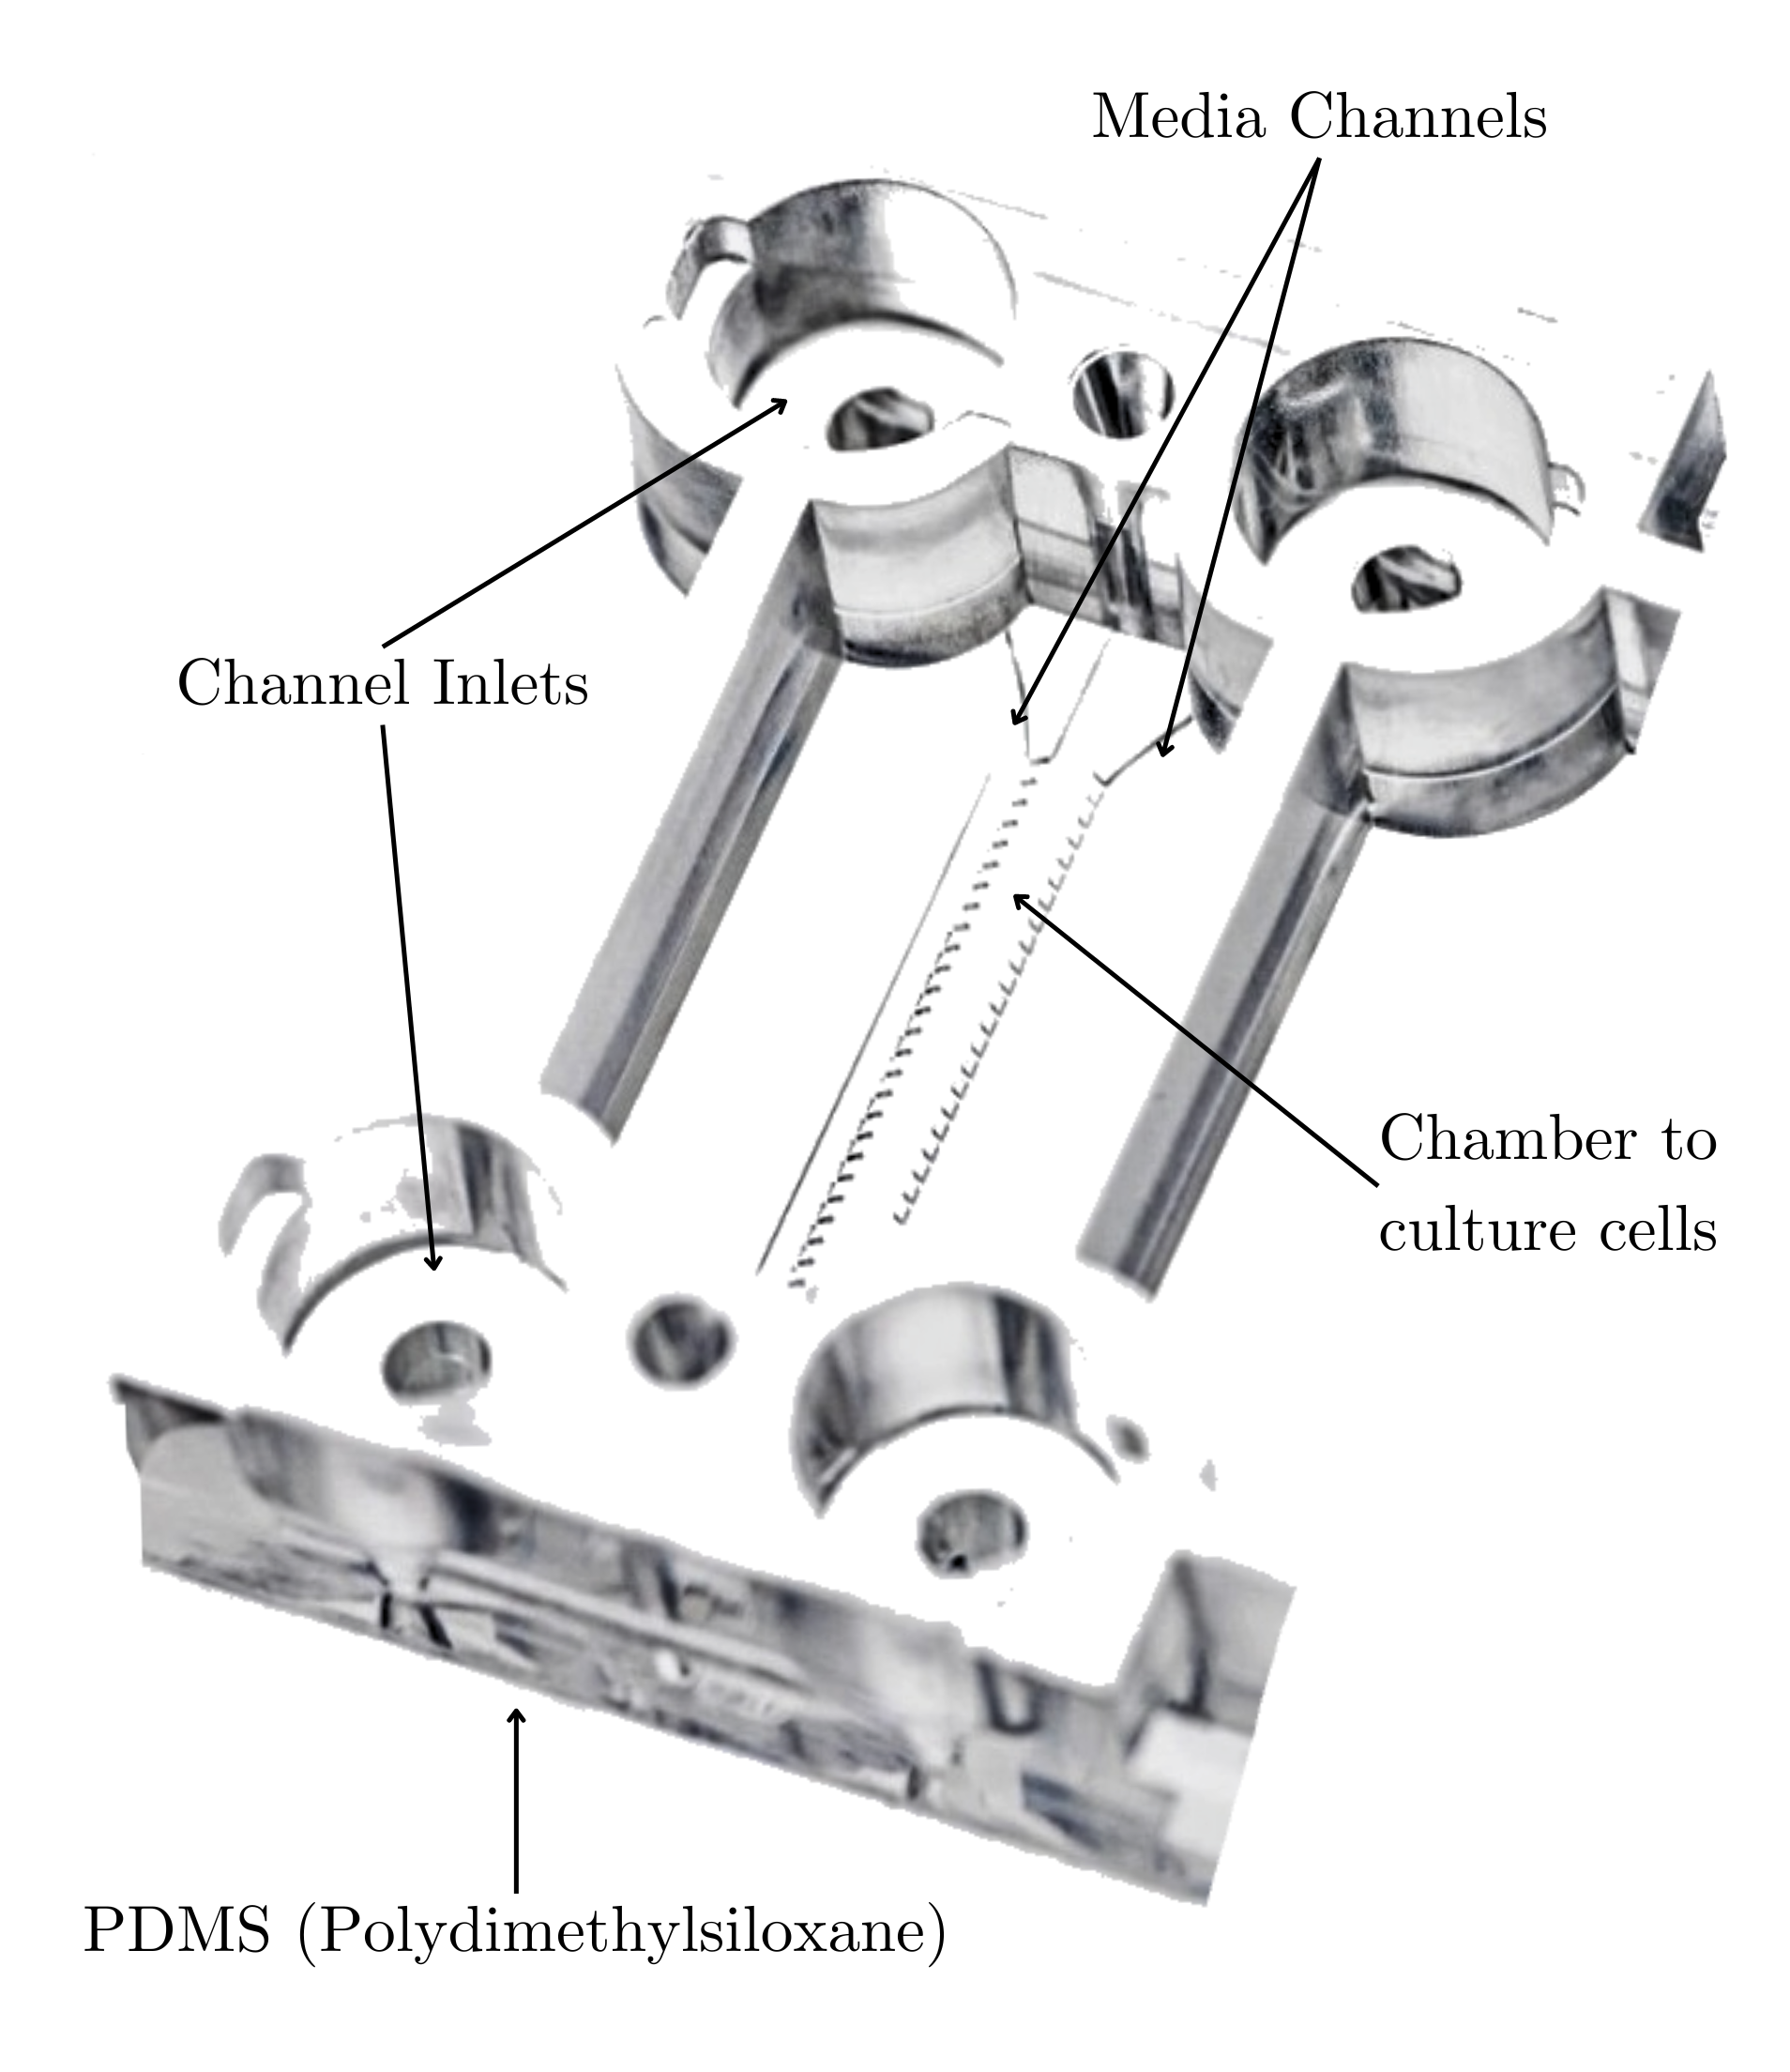
\includegraphics[width=0.5\textwidth]{dapp_report/figures/aim_chip.png} % Adjust the width as needed
    \caption{The above graphic shows an example AIM Biotech Microfluidic Chip with its respective components. Image taken from \cite{identx_3_chip_aim_biotech} }
    \label{fig:aim_chip}
\end{figure}

Microfluidic chips are a common class of devices used to mimic vascular networks \textit{in vitro}. These chips utilize microscale fluid channels to supply growth media, maintain optimal chemical and pressure gradients, and remove waste from cultured cells (Figure~\ref{fig:aim_chip}). Microfluidic chips hold an advantage over static petri-dish cultures, where deeper cells experience nutrient deprivation and waste accumulation. Moreover, by allowing for 3D cell culture, these chips support the morphophysiological requirements for most tissues to perform their normal functions \parencite{limongi_2022_microfluidics}. Typically, collagen matrices are used as scaffolding for endothelial cells to form a vascular network \parencite{oconnor_2022_engineering}.  Traditional microfluidic chip designs often do not have special features to support vasculogenesis or angiogenesis. Moreover, the channels present in these chips fail to recreate the natural vascular hierarchy - a progression from larger vessels to smaller vessels, culminating in capillary networks. Previous projects have achieved vasculogenesis, but the aim of this project is to create a central feeder vessel, with microvessels sprouting from it\parencite{quintard_2024_a}.  

\subsection{Existing Methods}
Various methods have been explored to achieve this goal: 

\begin{figure}[h]
    \centering
    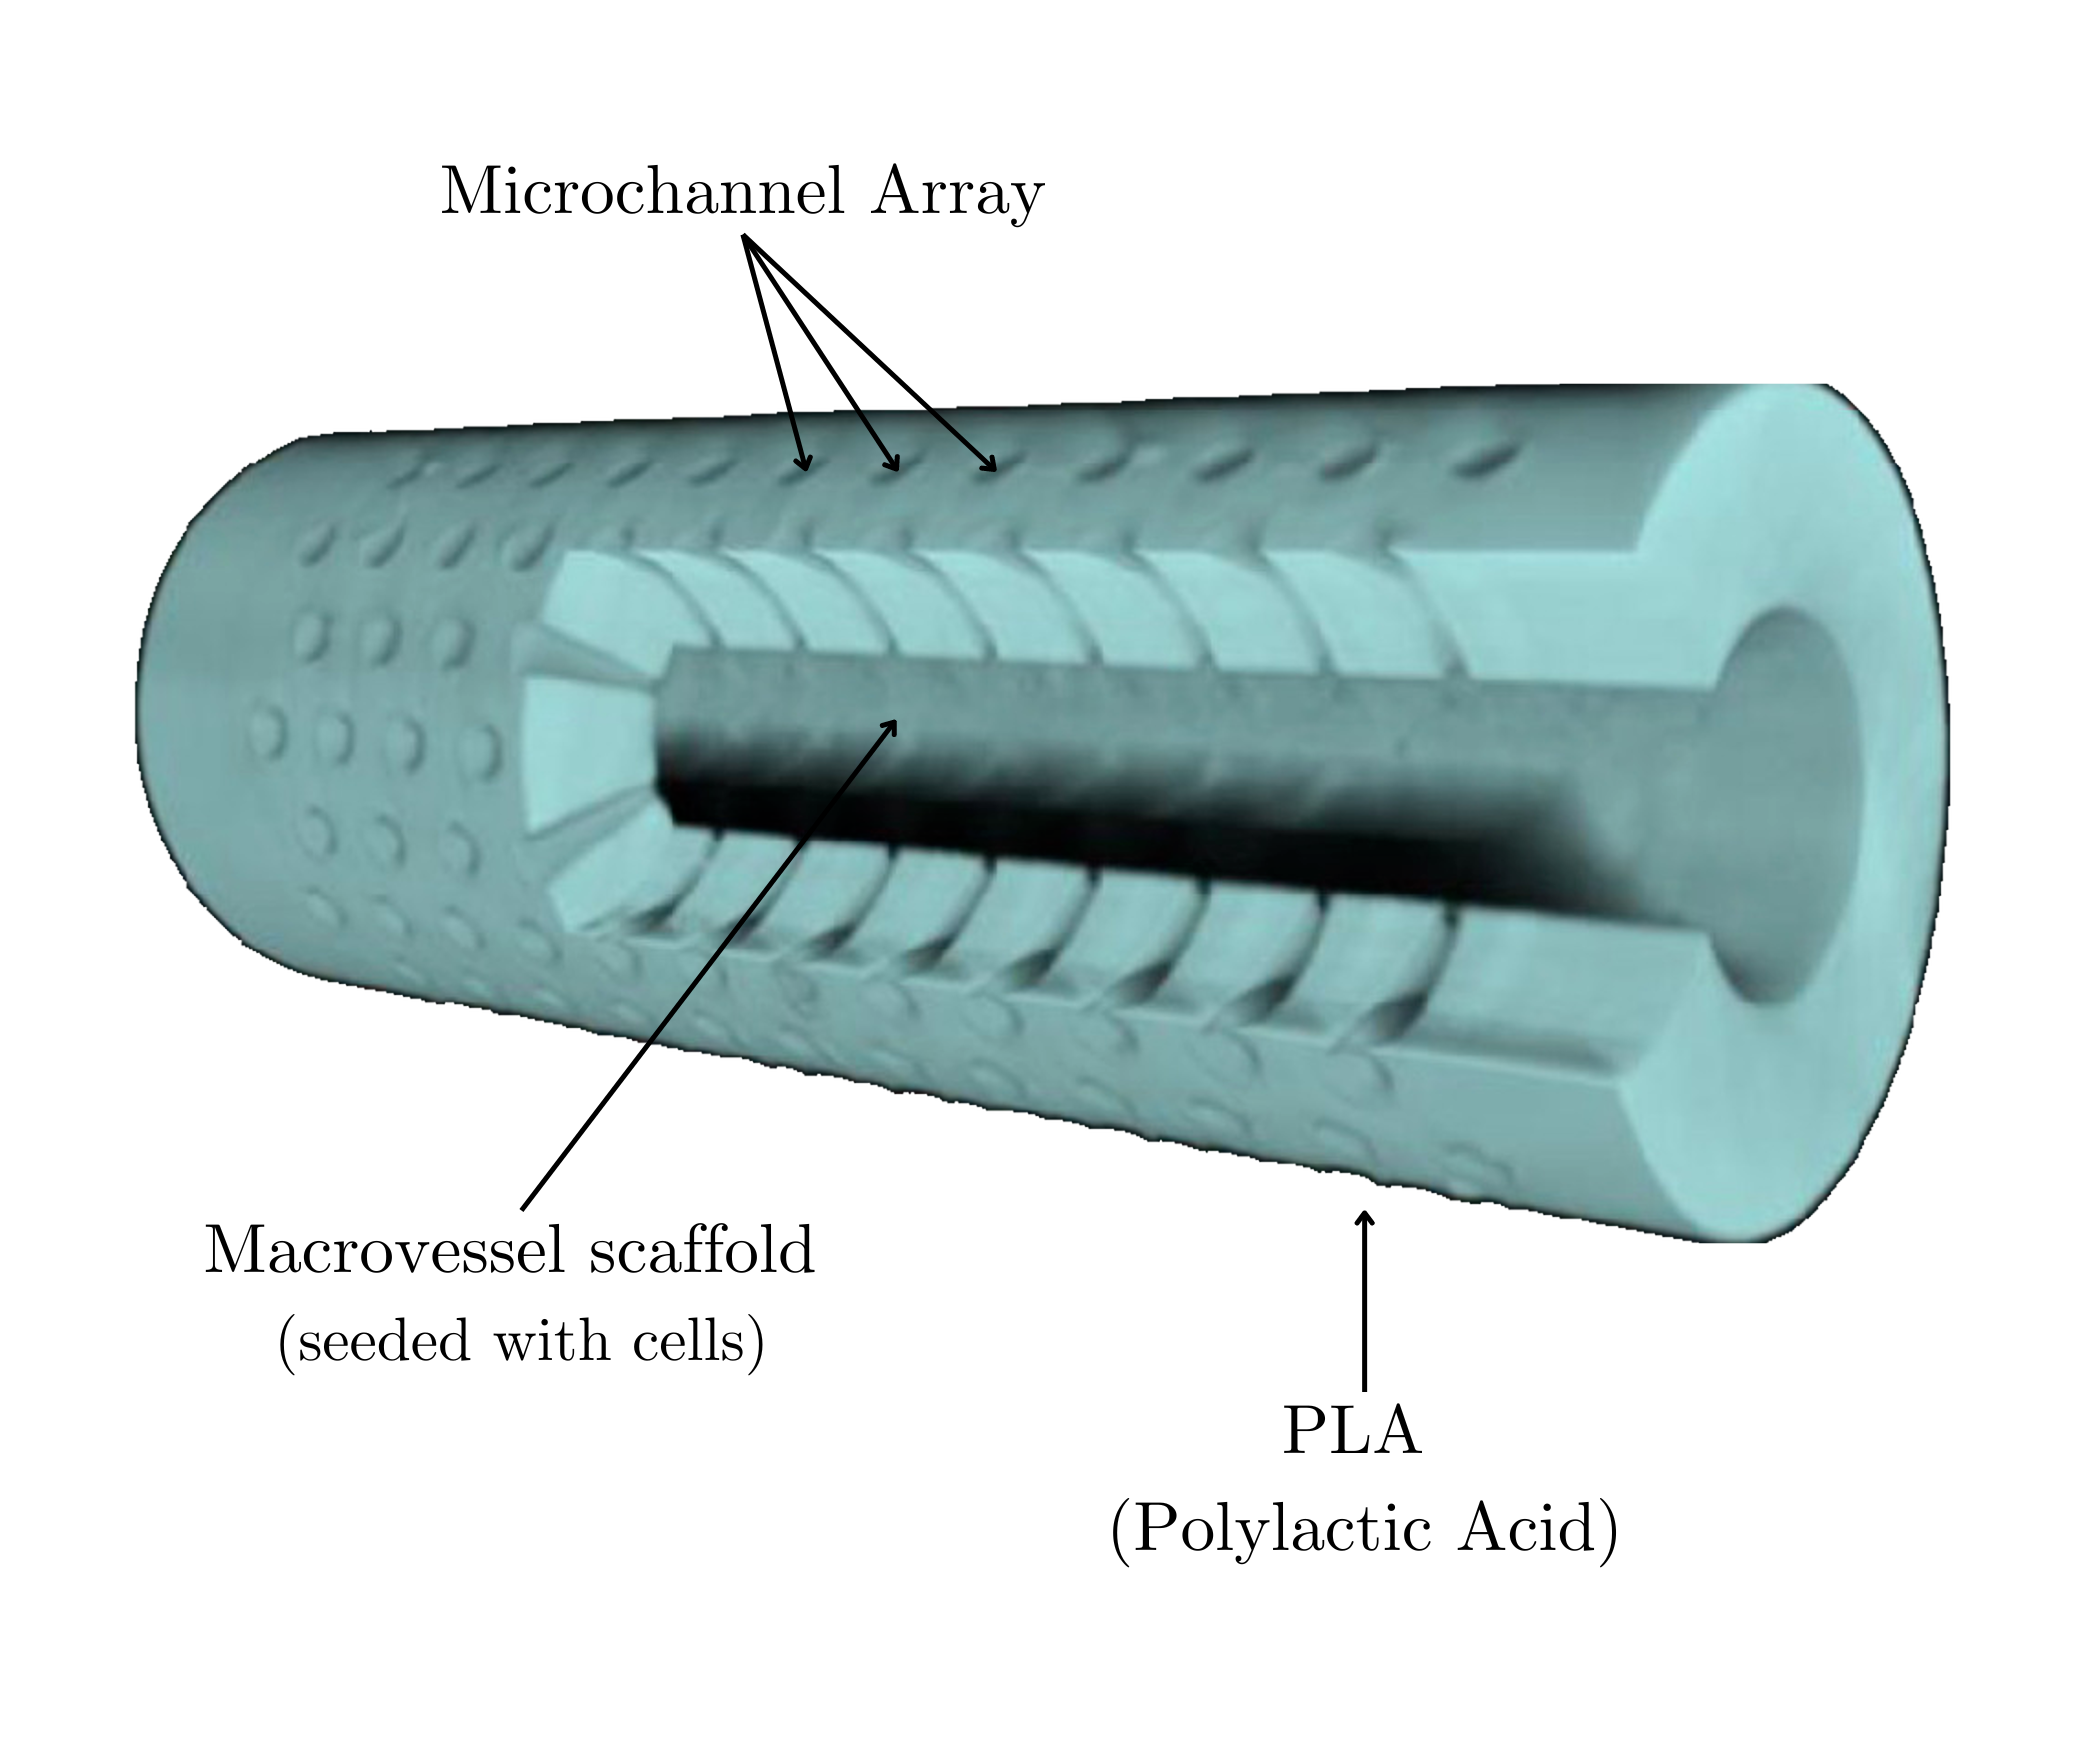
\includegraphics[width=0.5\textwidth]{dapp_report/figures/angiotube_method.png} % Adjust the width as needed
    \caption{The above graphic shows the Angiotube design highlighting the macro-vessel scaffold and micro-channel array. Image taken from \cite{zohar_2022_a} }
    \label{fig:angiotube_fig}
\end{figure}

\begin{itemize}
    \item \textbf{Silastic Tubing Method}: This method utilised a temporary scaffold around which vascular tissues were engineered. These tubes were inserted into the peritoneal cavity of rats or rabbits, which, after two weeks, became encased in a capsule composed of myofibroblasts, collagen matrices, and a mesothelium lining. The tubing acted as a mould, shaping the formation of these layers. Once harvested, the silastic tube was removed, and the tissue tube was everted, positioning the mesothelium internally to mimic the endothelium of a blood vessel\parencite{campbell_1999_novel}. 
    \item \textbf{Dynamic Perfusion in Hydrogels}: Human umbilical vein endothelial cells (HUVECs) were cultured and transferred onto a 3D-printed tubular scaffold. This cell sheet, once in place, was embedded within a collagen gel. Under dynamic conditions, the perfusion of growth medium through this setup allowed the embedded HUVECs to begin sprouting into micro-vessels, forming a dense, 3D vascular network throughout the gel\parencite{elomaa_2022_in}. 
    \item \textbf{Angiotube Method}: This system comprises a biodegradable macro-vessel scaffold, made of polylactic acid (PLA) surrounded by a cylindrical array of spacing for micro-channels to grow (Figure~\ref{fig:angiotube_fig}). The design facilitates the development of a central vessel channel while also supporting the growth of a capillary network through the embedded micro-channel spaces. When seeded with endothelial cells into the lumen of the macro-vessel, the cells vascularise and form multiscale networks\parencite{oconnor_2022_engineering}. 

\end{itemize}

These methods encounter several challenges, primarily the use of non-permeable scaffolds. This restricts the natural perfusability essential for endothelial cells to form capillary networks and guides the cells into a rigid 3D structure. Another limitation is the complexity involved in designing and fabricating such small-scale 3D scaffolds. For instance, the Angiotube method utilises a complex fabrication process, which includes precise picosecond laser drilling to create the microchannels\parencite{oconnor_2022_engineering}.

\subsection{Our Approach}

This report describes a microfluidic chip system designed to support the growth of multiscale vasculature within a permeable scaffold, incorporating semi-rigid structural constraints. This aims to address the design limitations outlined previously, while also simplifying the manufacturing and fabrication processes. By leveraging the self-organisation capabilities of HUVECs, we can create a scaffold for a central feeder vessel, which will sprout smaller microvessels.  
\newpage

\section{Requirements Definition}

The microfluidic chip (the chip) aims to support the growth of a multiscale blood vessel network. The chosen approach involves incorporating a hydrogel chamber for culturing cells in a contaminant-free environment, supported with adequate growth media and waste collection mechanisms, while facilitating imaging under a microscope. To align with overall requirements, the chip must meet specific design and manufacturing criteria.

\begin{itemize}


    \item \textbf{Chip Material:} The chip material must be biocompatible. It should be optically clear, easy to image, and capable of being moulded into the required design geometry. 

    \item \textbf{Hydrogel:} The hydrogel must be non-cytotoxic and permit proper light penetration to ensure high optical clarity during imaging. The gel should also be permeable to growth media and other necessary fluids. 


\item \textbf{Hydrogel Chamber Design:} The hydrogel should be contained within an enclosed chamber to reduce the likelihood of contamination and ensure stability while handling the chip. The design should facilitate the insertion of a needle into the chamber before injecting the hydrogel while preventing leakage. This supports a crucial feature of the gel chamber design - the injection of cells via the inserted needle once the gel has set. 


    \item \textbf{Side Channel Design:} The chip should include two side channels (one media and one waste channel), adjacent to the gel chamber, which guarantees even distribution of media across the hydrogel. This establishes the necessary chemical and pressure gradients. These channels should prevent bubble formation or allow for the expulsion of bubbles without entrapment. Channel interfaces must also prevent hydrogel leakage while allowing free media flow. The rigidity and size of the inlets should be sufficient to accommodate external reservoirs containing cell media. 

    \item \textbf{Media and Waste Reservoirs:} The chip should be compatible with detachable liquid reservoirs (i.e. pipette tips) for supplying cell media (with growth factors) and waste collection. These reservoirs should not cause leakage; they should be simple to replace throughout the experiment and remove during imaging. 

    \item \textbf{Size:} The chip must be compact enough to fit on a standard microscope slide and suitable for imaging with standard commercial microscopes. 

    \item \textbf{Ease of manufacture:} The chip should be sufficiently robust to prevent the collapse of individual features. It must be manufacturable in a consistent, cost-effective manner to ensure uniformity within and across batches for repeat experiments. It should not include very tall or thin features to maximise success of PDMS casting and reduce mould damage. 

    \item \textbf{Usability Requirements:} The chip must remain thermally stable over experimental periods (2 weeks), under experimental conditions (inside a cell incubator), and withstand thermal sterilisation techniques. It should be chemically inert, not leach cytotoxic materials, and comply with standard biohazard waste and sharps disposal protocols. 

\end{itemize}

% \newpage
\newpage
\section{Final Design}
\subsection{Final Design features}

The chip is made of PDMS (Polydimethylsiloxane). It contains a central chamber with a flat, smooth ceiling, where the hydrogel is injected and set. The chip features one media channel and one waste channel, each equipped with two inlet holes. The presence of the second inlet allows for the expulsion of air and any bubbles. This configuration enables the media, which contains growth factors and nutrients, to permeate the entire length of the hydrogel. This specific arrangement of channels facilitates the establishment of lateral pressure gradients across the hydrogel, promoting vasculogenesis and, subsequently, angiogenesis. To constrain the hydrogel while maintaining unimpeded media flow, phase guides are employed, utilising the meniscus pinning effect\parencite{vulto_2011_phaseguides}. In microfluidics, the meniscus pinning effect describes the phenomenon of liquids being “pinned” to surfaces due to their surface tension overcoming the force of capillary action\parencite{wetting_forces}. As long as there is negligible advection pressure, it is energetically favorable for a liquid to remain pinned to an angled surface rather than create further surface wetting. This principle is used to constrain the flow of hydrogel\parencite{wetting_forces}. The phase guides must meet the meniscus pinning and \textit{Concus-Finn} criteria to function properly, thus employing a maximum interaction angle of 90°. The chip is then mounted on a glass slide, which has a smooth, flat, and transparent surface, allowing for direct microscopic imaging without further modification. A detailed breakdown of the chip’s features can be found in Table~\ref{tab:chip_design} and in Figures~\ref{fig:tech_draw_chip_final} and \ref{fig:3d_render_microchip}.

\begin{figure}[h!]
    \begin{minipage}[b]{0.33\textwidth}
        \centering
        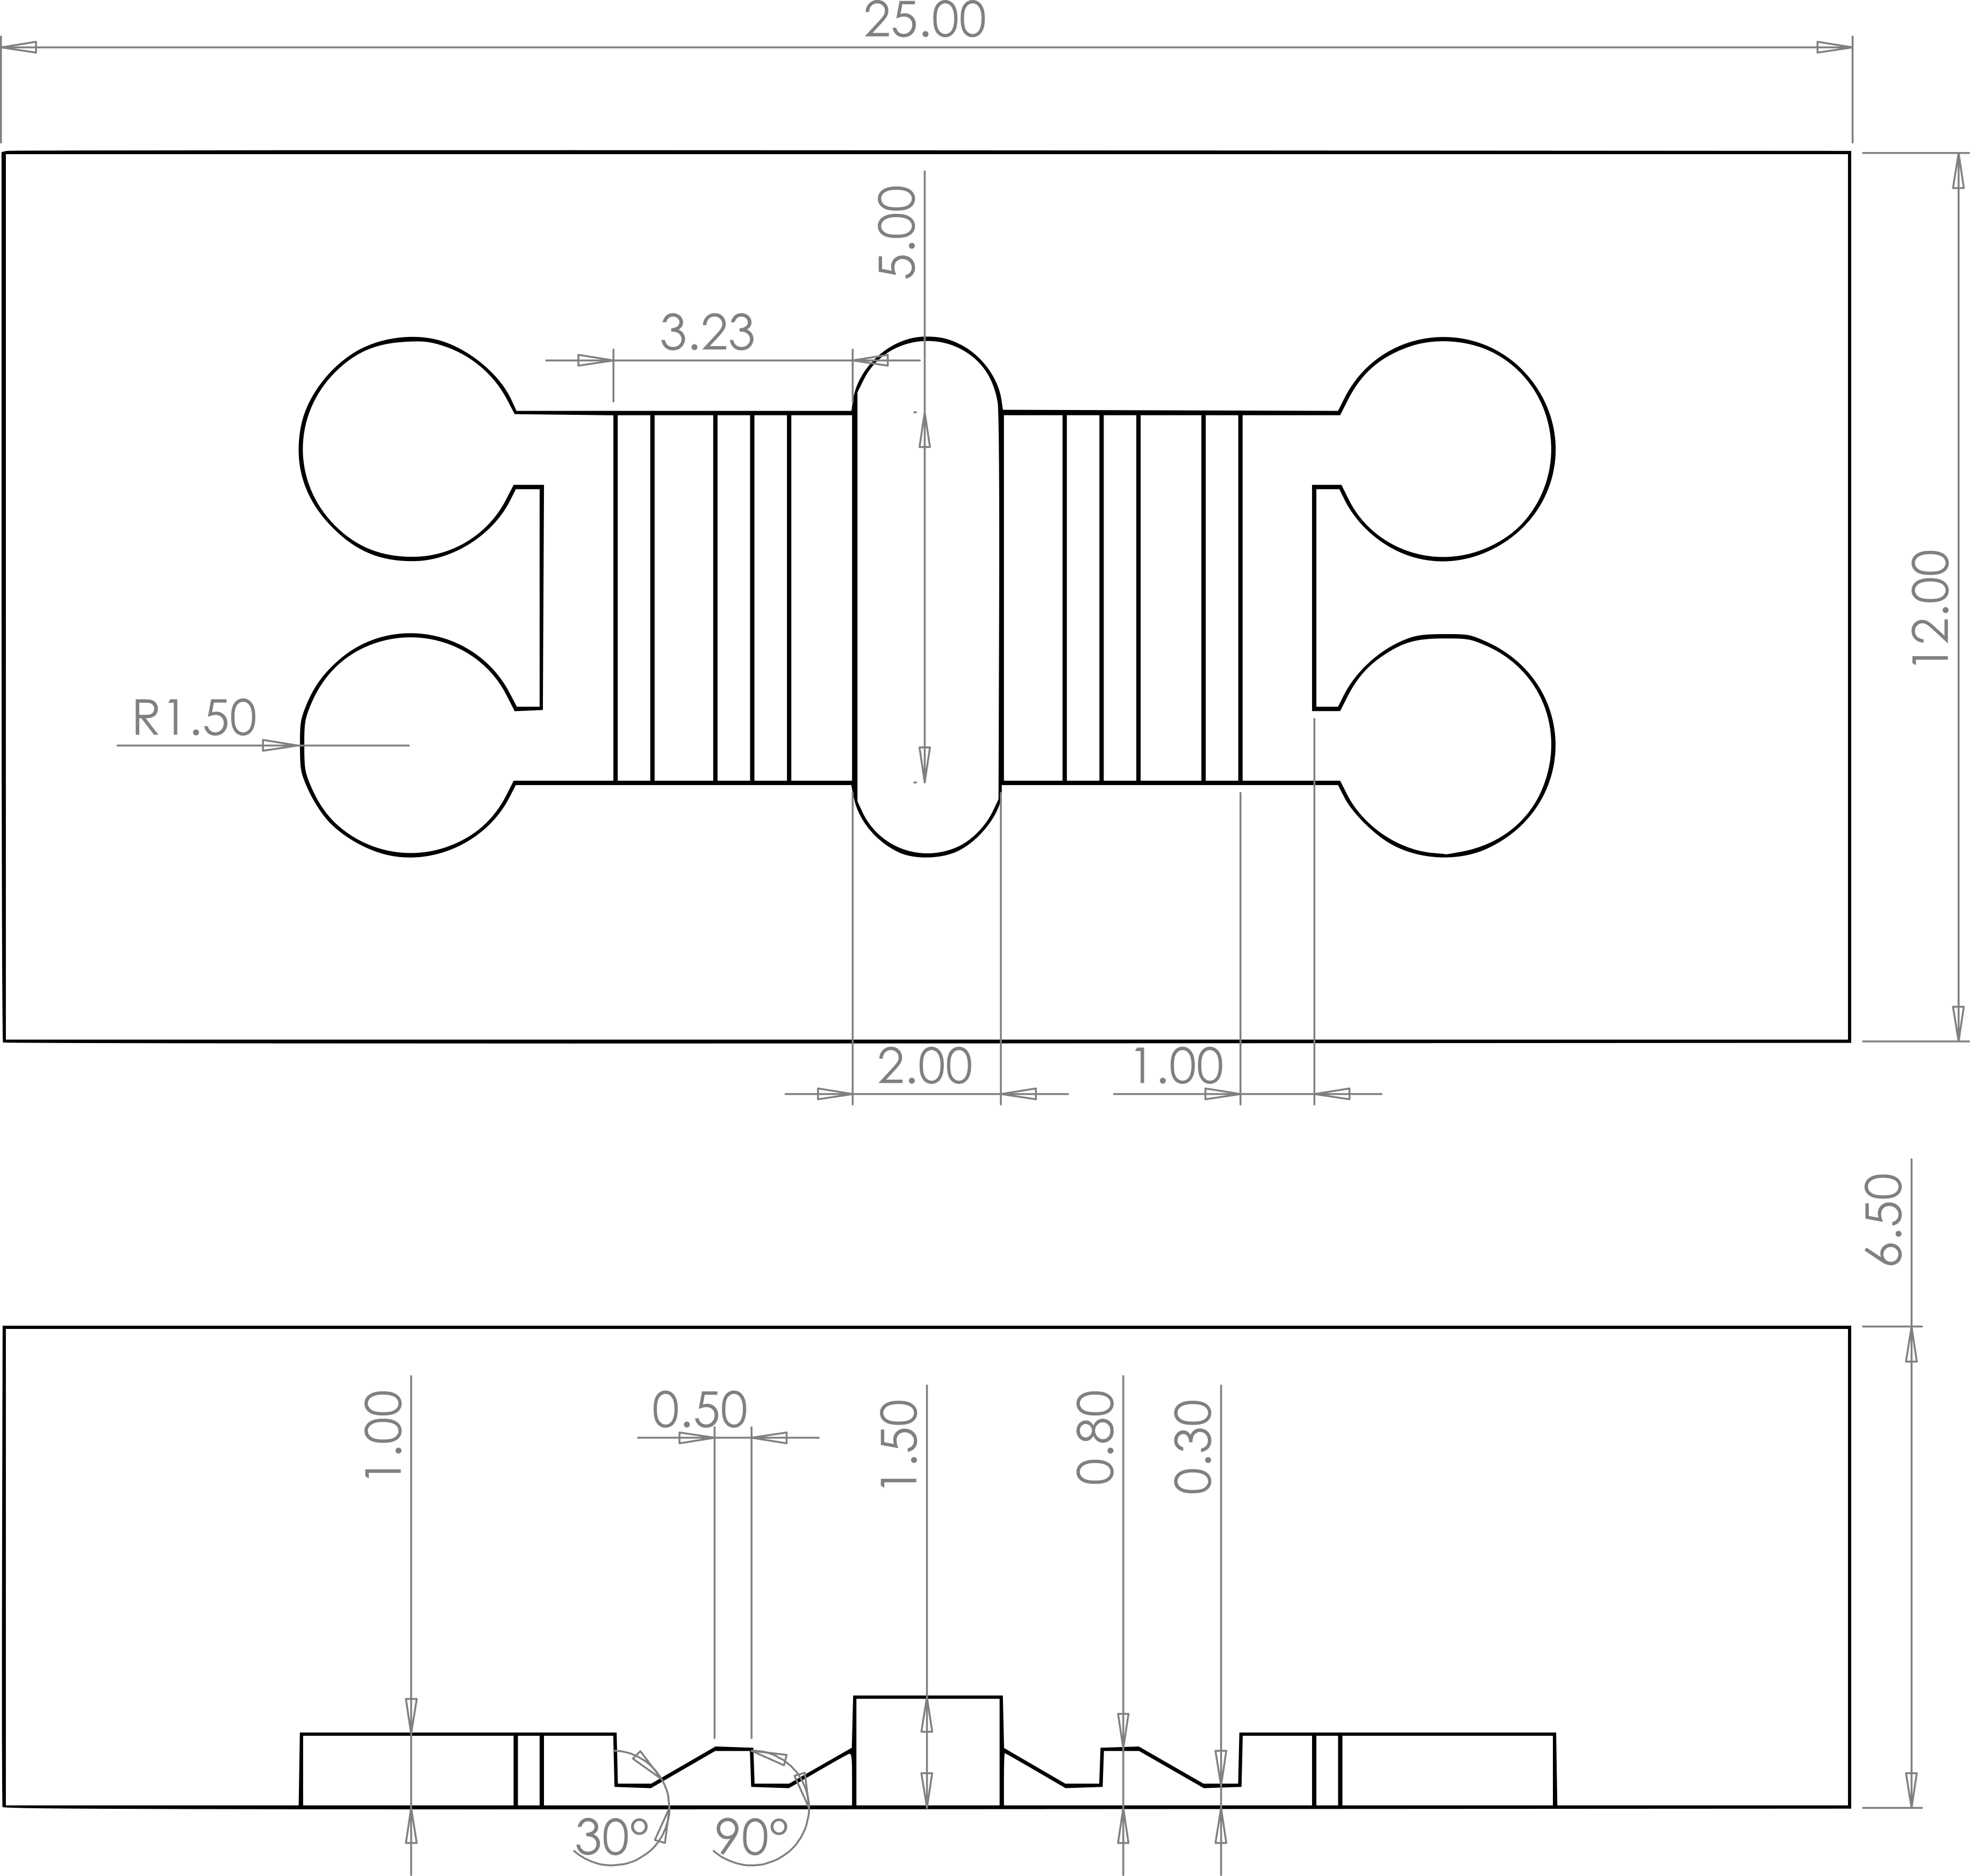
\includegraphics[width=\textwidth]{figures/Chip_technical_drawing.png}
        \caption{Technical Drawing of the chip}\label{fig:tech_draw_chip_final}
    \end{minipage}
    \hfill
    \begin{minipage}[b]{0.6
    \textwidth}
        \centering
        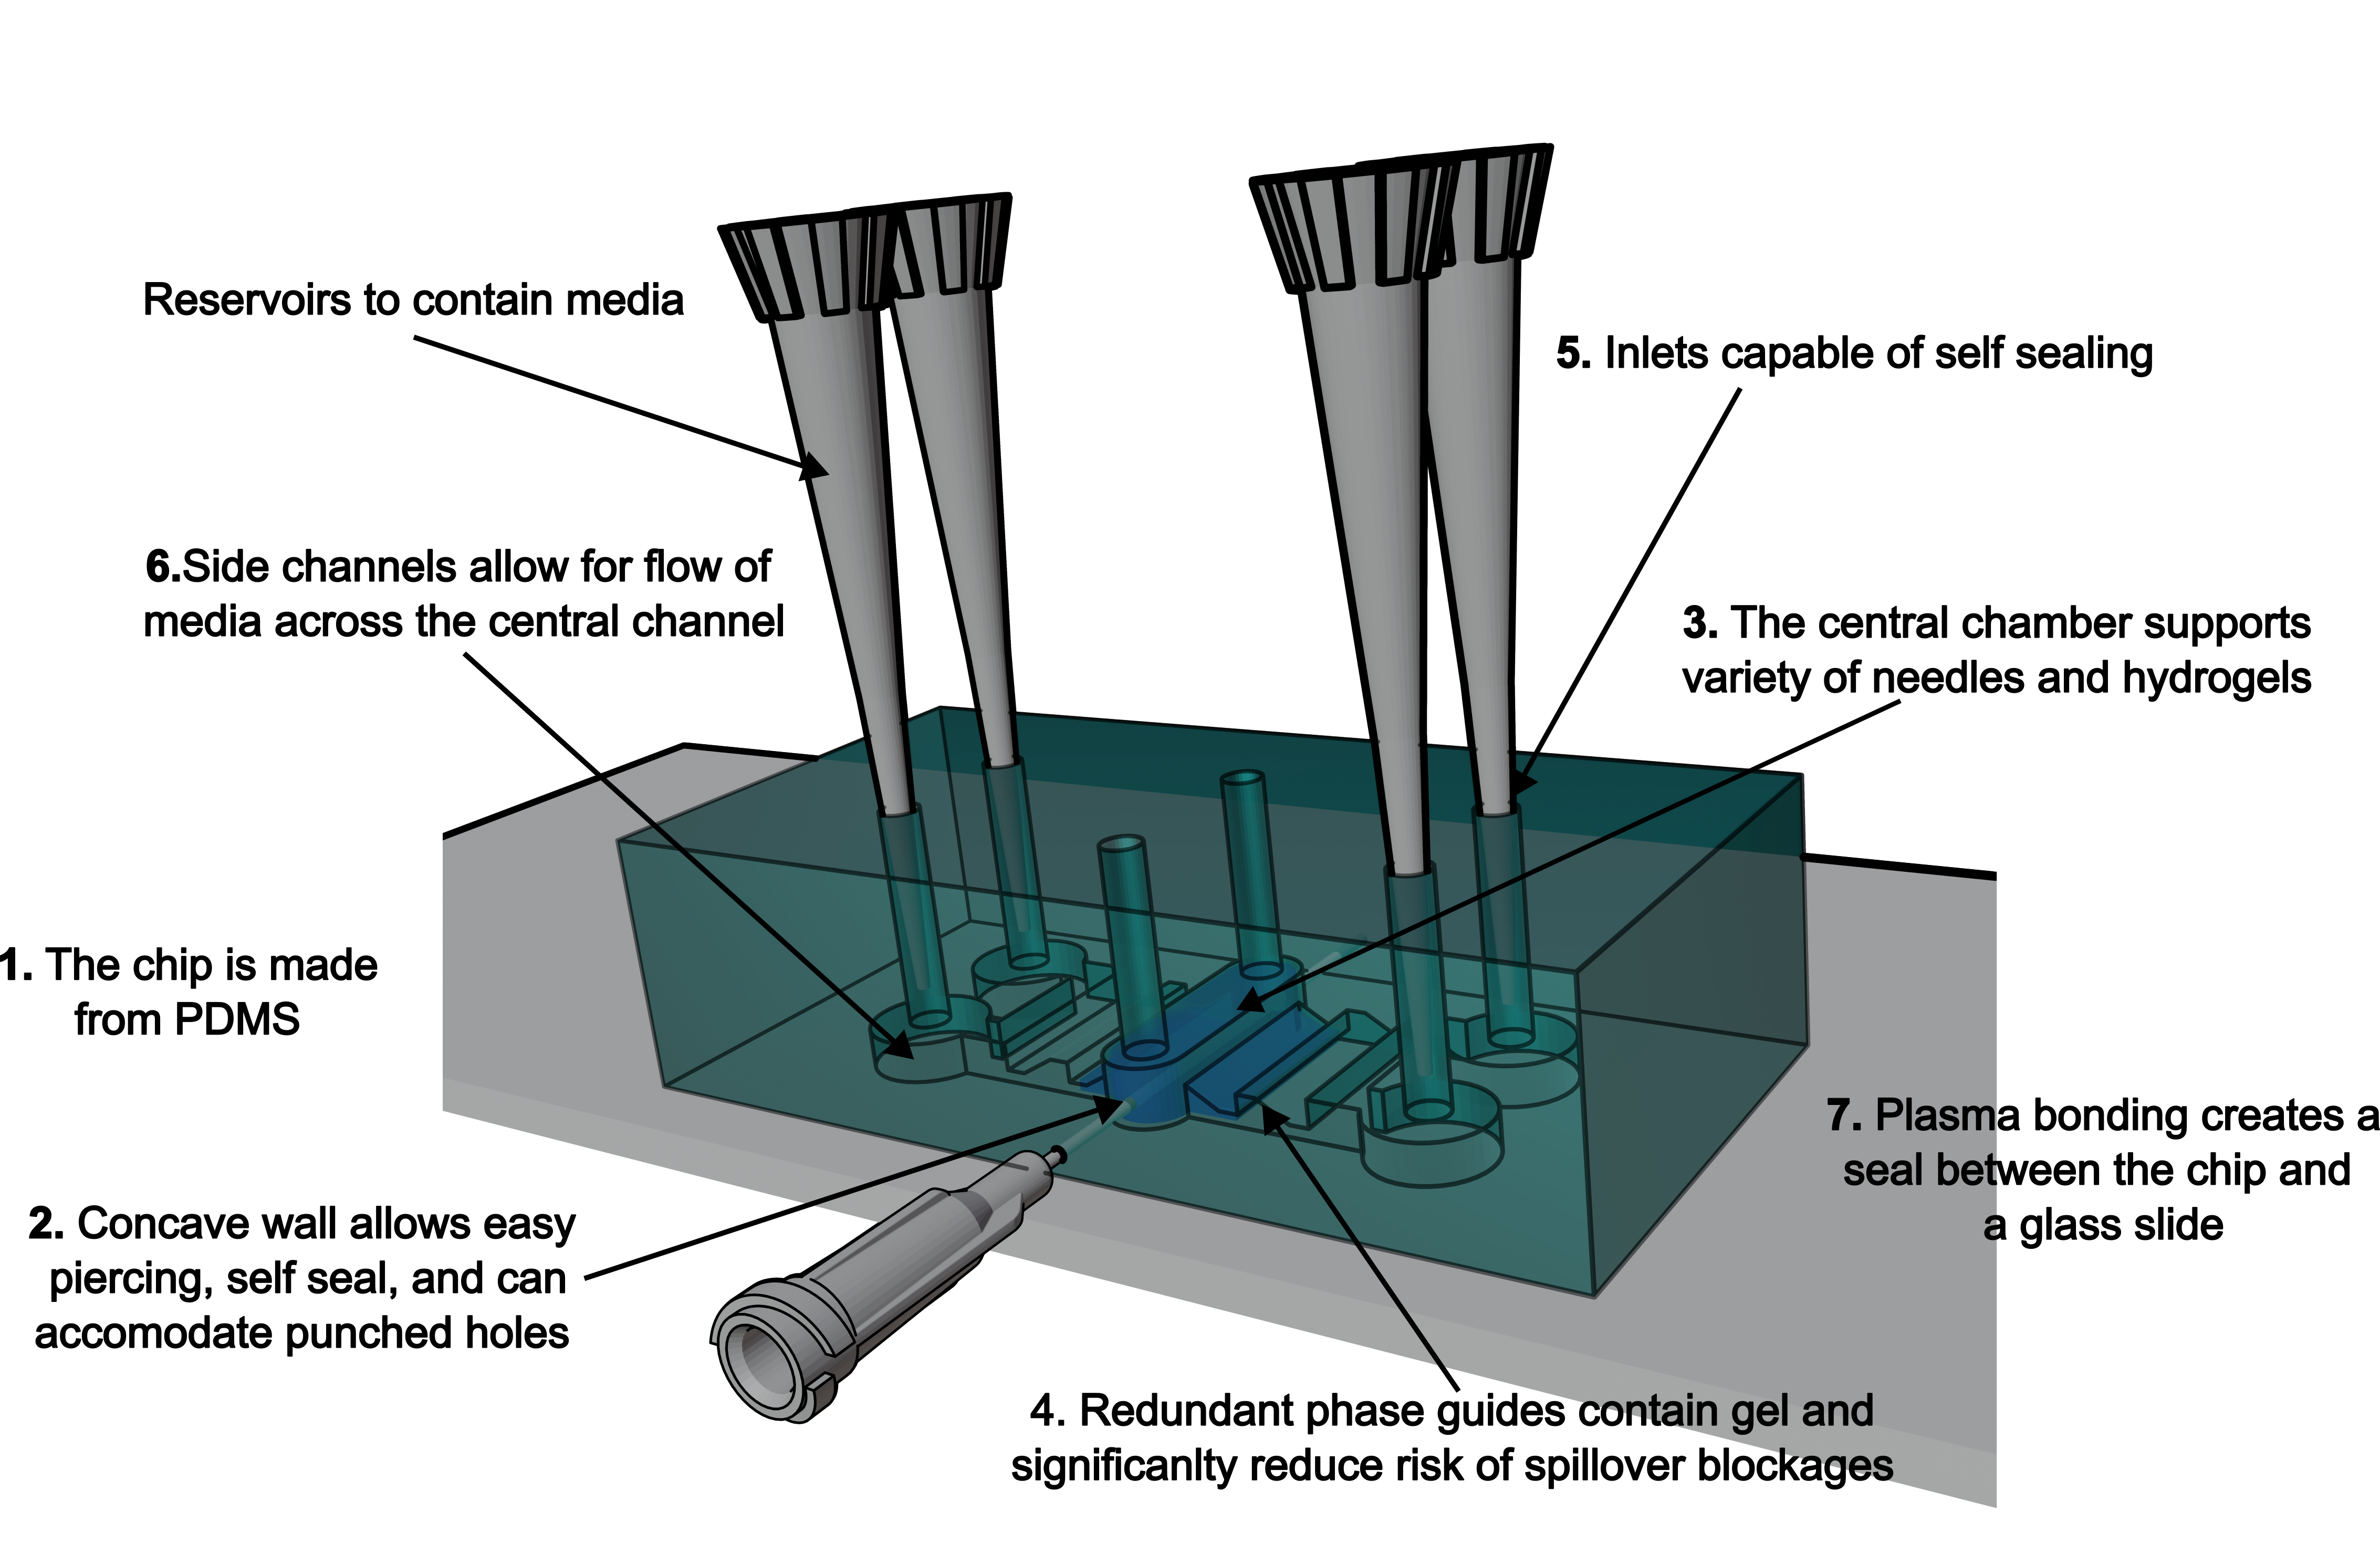
\includegraphics[width=\textwidth]{figures/annotated_features.png}
        \caption{3D Render of the Microfluidic chip}\label{fig:3d_render_microchip}
    \end{minipage}
\end{figure}


\newgeometry{left=1cm,right=1cm, bottom =2cm, top = 2cm}


\begin{table}
    \footnotesize
    \setlength\tabcolsep{1pt}
    \centering
    \captionsetup{justification=centering}
    \caption{Design features and properties of the final chip design}\label{tab:chip_design}
    \begin{tabularx}{\columnwidth}{|c|
        >{\centering\arraybackslash}m{1.5cm}|>{\centering\arraybackslash}m{2.3cm}|
        >{\centering\arraybackslash}m{2cm}|>{\centering\arraybackslash}m{2.7cm}|
        >{\centering\arraybackslash}m{2.3cm}|>{\centering\arraybackslash}m{2.5cm}|
        >{\centering\arraybackslash}m{2.6cm}|>{\centering\arraybackslash}m{2.5cm}|}
\hline
\
\textbf{\#}  & \textbf{Design Features}  & \textbf{Function}  & \textbf{Optical Properties}  & \textbf{Mechanical properties}  & \textbf{Chemical properties}  & \textbf{Cost}  & \textbf{Versatility}  & \textbf{Usability}  \\
\hline
\hline
\textbf{1}  & \textbf{PDMS} as the Chip Material  & Material supports other design features. Easy to cast and modify.  & Transparent High clarity Low aberrations.  & Elastic yet firm, allows easy modification and piercing even after fully curing. Tear and shatter resistant.  & Polymerised. Hydrophobic, thermally and chemically stable over operative timescale.  & Cost effective in smaller scales. Process of casting is cheap. Mould is reuseable.  & High versatility. Allows easy modifications.  & Relatively easy to mould with a negative. Results are generally easy to reproduce.  \\
\hline
\textbf{2}  & Concave gel chamber walls  & Allows puncturing by a needle and injection of cells into hydrogel.  & N/A  & Elastic and flexible, easily pierced by a variety of needles while maintaining a firm seal.  & N/A  & Cast directly into the chamber, much cheaper than using separate fluid seals.  & Highly versatile - accommodates various needles without changes to design.  & Easy to pierce through. Tapered shape can be used for alignment.  \\
\hline
\textbf{3}  & Enlarged Gel chamber  & Provides hydrogel loaded environment for cell culturing.  & Smooth surface allows visualisation of bulk gel without interference.  & Allows loading of a large “block” of gel which prevents collapse of hollow central channels.  & N/A  & Very low cost. Marginal reduction in material cost.  & Highly versatile. Leaves plenty of room for imaging regardless of needle gauge.  & Easy to use. Large margin for potential errors without ruining the sample.  \\
\hline
\textbf{4}  & Double Phase guides  & Contains unset hydrogel to central channel during injection but allows flow of nutrient media and growth factors.  & N/A  & Shape makes it resistant to bending and tearing, unlike microposts. Simplifies extraction of the microchip from mould.  & High contact angle between PDMS and hydrophilic fluids is essential for fulfilling the Concus–Finn criterion.  & Medium cost. Requires greater precision when making a mould to ensure the correct fluid interactions.  & Low versatility, effectiveness highly dependent on the properties of gel and media. Requires highly viscous gel to be used.  & Requires great precision while loading - once bypassed, phase guide stops functioning
; thus secondary guide is included.  \\
\hline
\textbf{5}  & Media inlets and outlets  & Allows loading and removal of nutrient media.  & N/A  & No effect on structural integrity. Strong enough to hold the reservoirs.  & N/A  & Very low cost. Made using a biopsy punch.  & Highly versatile. Allows mounting of a variety of reservoir sizes. Radius can be varied.  & Easy to use. Red and yellow pipette tips can be used without adhesive.  \\
\hline
\textbf{6}  & Side channels  & Provides lateral flow between media inlets and hydrogel channel.  & N/A  & Shape allows to distribute media flow across the length of hydrogel.  & N/A  & Very low cost as it is a part of casting procedure.  & Inbuilt shape. Modifications require change to mould.  & Easy to mount reservoirs to and affix with adhesive.  \\
\hline
\textbf{7}  & Plasma Bonding between chip and glass slide  & Forms a watertight seal and allows imaging in most commercial microscopes.  & Transparent and high clarity, low aberrations.  & Strong watertight seal. Dimensions are compatible with most microscopes.  & Requires no adhesives. Plasma cleaning process decontaminates the surface.  & Glass slides are highly cost effective. Low overhead costs with available machinery.  & Highly versatile, allows any number of chips to be adhered to any glass surface including plates if needed.  & Easy to perform. Low risk of losing adhesion over operating time frame.  \\
\hline

\hline
\end{tabularx}
\end{table}



\restoregeometry


\newpage


\begin{figure}
    \centering
    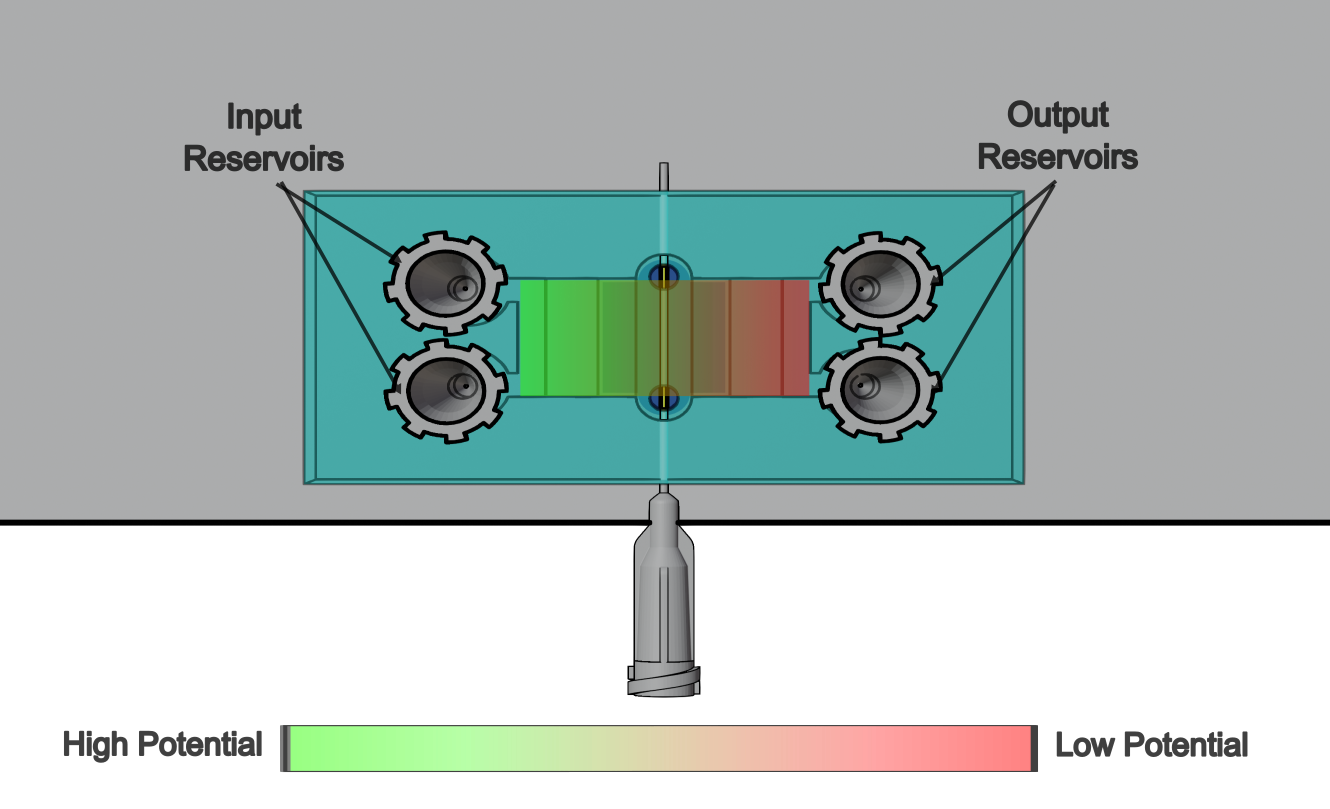
\includegraphics[width=0.4\linewidth]{figures/potential gradient.png}
    \caption{Ideal pressure and chemical potential distribution}
    \label{fig:pressure gradient}
\end{figure}


\subsection{Manufacturing}
\begin{figure}[h!]
    \centering
    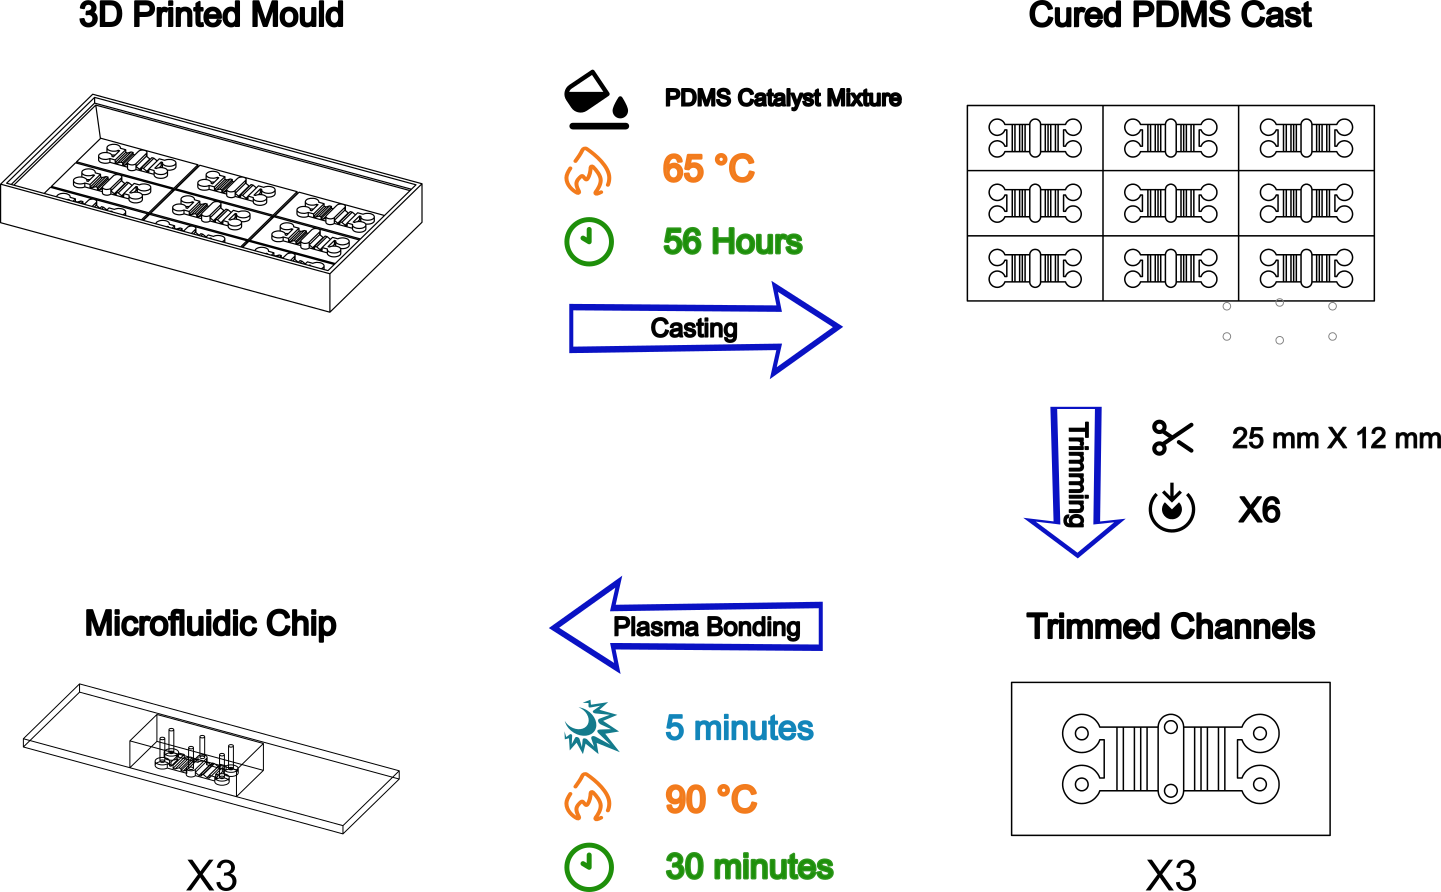
\includegraphics[width=1\textwidth]{figures/manufacture_procedure.png}
    \caption{Different stages of the manufacturing process as listed below.}\label{fig:manufac}
\end{figure}

\newpage
The manufacturing process was structured into four different stages (Figure~\ref{fig:manufac}):

\begin{enumerate}
\item \textbf{3D Printing the Mould:} The process begins with the mould being 3D printed in resin using a masked stereolithography apparatus (MSLA) which allowed for a smooth surface that minimised optical aberrations. The mould material needed to be chemically inert to PDMS,  thermally stable up to 65°C, and have hydrophobic properties\parencite{a2019_elegoo}, to prevent the chip from sticking to the mould. Elegoo Standard Photopolymer Resin™ was chosen for its cost-effectiveness, availability, and suitability for single-use moulds. The mould was cleaned using 99.9\% isopropyl alcohol to remove any uncured resin; it was then cured under UV light for a minimum of 15 minutes. The design details of the mould can be found in Figure \ref{fig:manufac}.

\item \textbf{Casting with PDMS:} A mixture of liquid PDMS base and a curing agent was degassed in a vacuum chamber, poured over the mould, and cured in an oven at 65°C for approximately two days. The chips were then carefully removed from the mould to avoid any tearing. 

\item \textbf{Post-processing:} The chips were cut along specially designed lines inside the mould. Holes for the central channel and side channel reservoirs were produced using a 1.5mm biopsy punch. This method was adopted because moulds with pre-formed holes complicate the removal of the cast chips. 

\item \textbf{Plasma Bonding to Microscope Slide:} In the final stage, the chips were attached to microscope slides via plasma bonding. This involved a brief plasma treatment of 20 – 30 seconds followed by 15 minutes on a 90°C hot plate. This technique does not require any reagents as it uses high-voltage induced radicals instead of adhesive, thereby avoiding biocompatibility issues and establishing a strong, water-tight bond with the glass surface. 

\end{enumerate}

\subsection{Chip setup protocol}
The following protocol is to be carried out upon successful manufacturing of a working microfluidic chip, which is tested according to the protocol in section \ref{manufacture_test}. 
\begin{enumerate}
    \item To set up the chip, a 32-gauge (different diameters could be used) needle is pierced through the center of the hydrogel chamber to support the formation of a tunnel through the hydrogel scaffold.  
    
    \item Next, 20 mg/mL fibrinogen is mixed with an equal volume of 4 U/mL thrombin and quickly injected into the gel chamber around the needle.  
    
    \item After injecting the hydrogel, the chip is incubated at 37 °C for 30 minutes to cure the hydrogel. 
    
    \item Once cured, the needle inside is used to inject the HUVECs, with the tunnel cast by the needle serving as the initial implantation surface to grow the central feeder vessel. Rotation of the chip is implemented to encourage the cells to line the tunnel’s walls, thus creating a larger capillary from which smaller microvessels can sprout into the surrounding hydrogel. 
    
    \item The cells should be cultured over several days at 37°C with 5\% CO2 and imaged at regular intervals under a microscope.   
\end{enumerate}


\subsection{Slide Rotator}

To ensure adequate HUVEC adhesion to the surface of the tunnel left by the needle, it was initially envisaged that an individual would periodically rotate the chip over 30-minute intervals.  The manual rotation of the chips was an anticipated problem that was not only arduous but could result in differences between chips. An initial 3D printed PLA slide rotator prototype was created where five chips could be loaded simultaneously into a rack and rotated on the rack’s octagonal edges (Figure \ref{fig:Rotator1}). This design still required rotating manually every few minutes, so the second PLA/acrylic slide rotator prototype was designed such that chips could be loaded and then rotated autonomously (Figure \ref{fig:Rotator2}). This was realised using a Nema 17 stepper motor driven by a L298N Dual H Bridge control board and an Arduino; the housing was constructed from 3D printed and laser cut parts with a large on/off button for easy control whilst working in a laboratory.

\begin{figure}[h]
    \begin{minipage}[b]{0.45\textwidth}
        \centering
        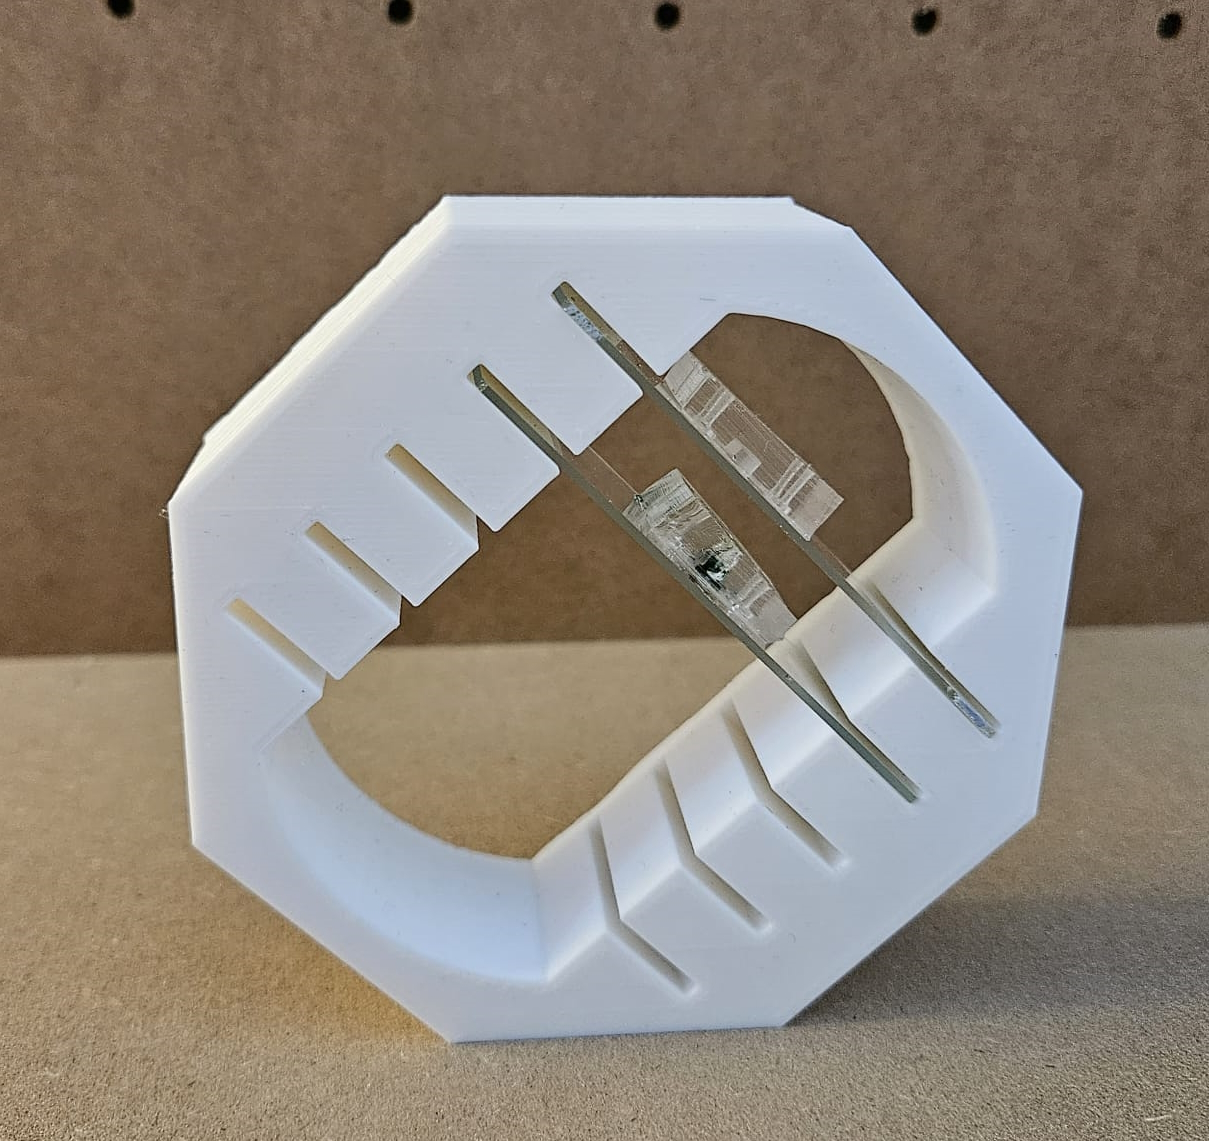
\includegraphics[width=\textwidth]{figures/Rotator1.jpg}
        \caption{Rotator Version 1}\label{fig:Rotator1}
    \end{minipage}
    \hfill
    \begin{minipage}[b]{0.4
    \textwidth}
        \centering
        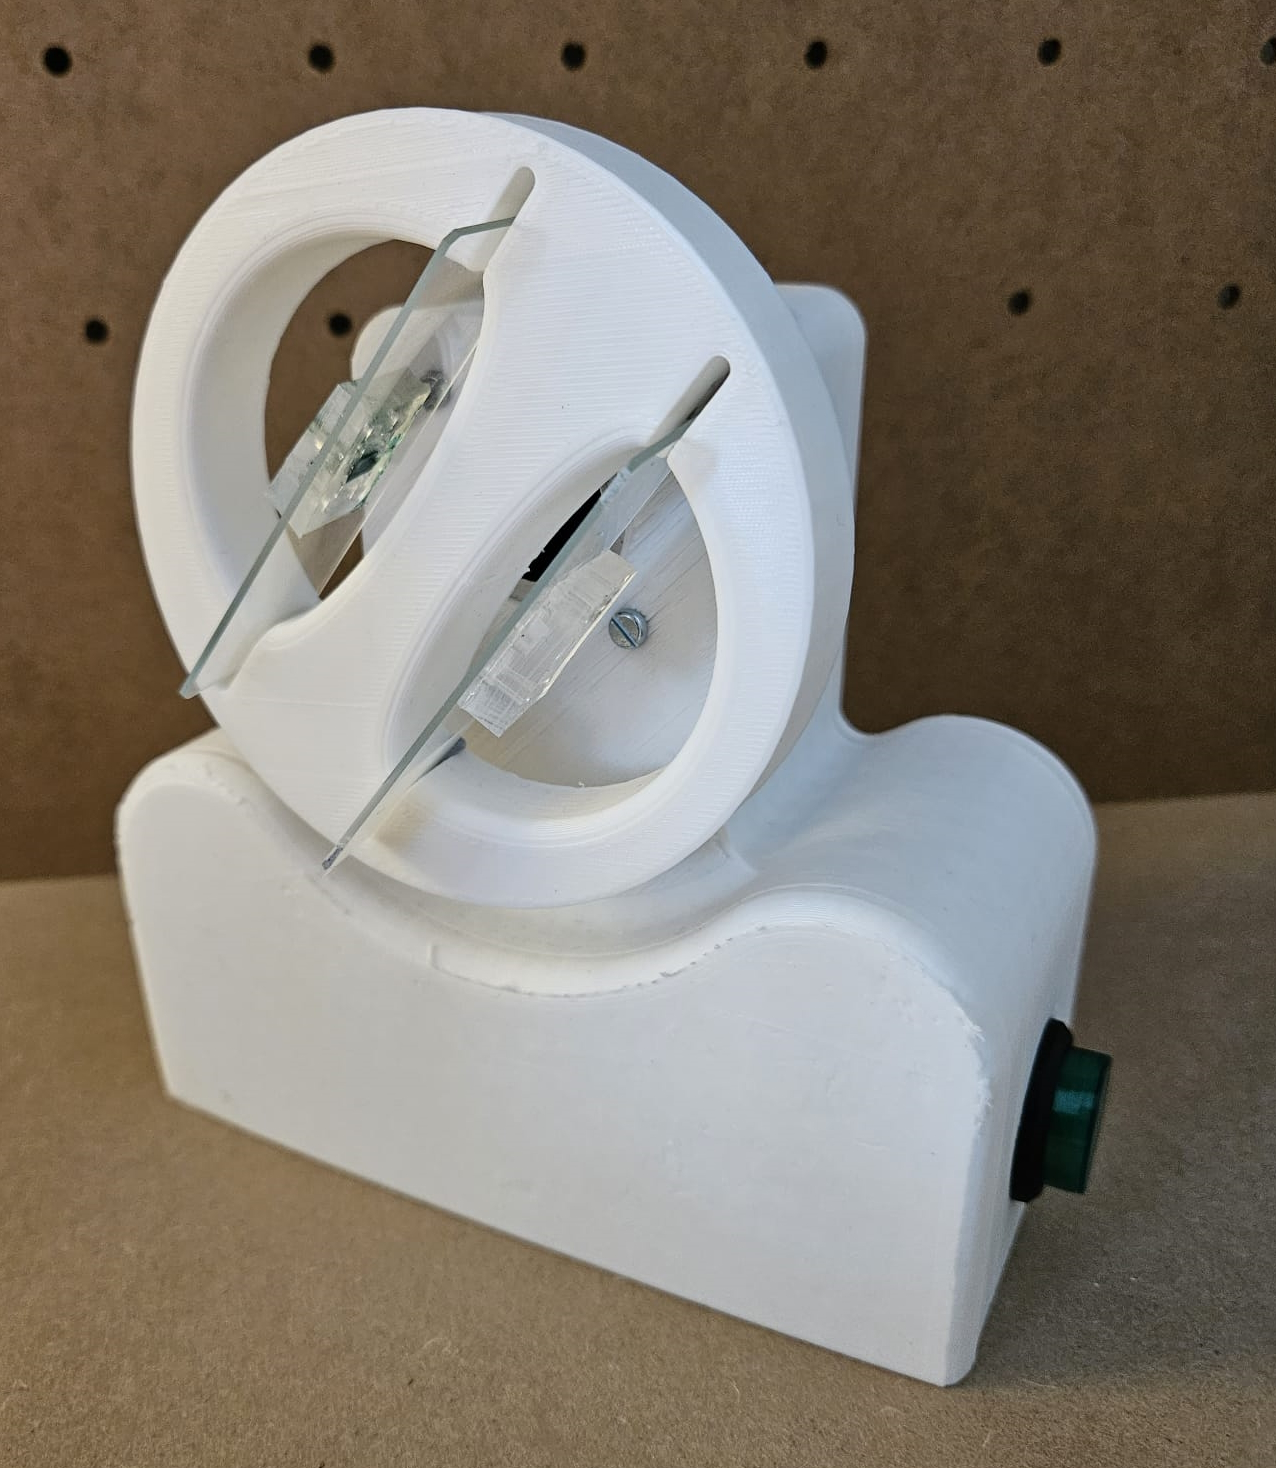
\includegraphics[width=\textwidth]{figures/Rotator2.jpg}
        \caption{Rotator Version 2}\label{fig:Rotator2}
    \end{minipage}
\end{figure}



\section{Discussion}
\subsection{Manufacturing}

\subsubsection{Methods of testing manufacturing} \label{manufacture_test}  

Before the full cell culturing protocol, the microfluidic chip should be checked to ensure correct manufacturing and functioning. After PDMS casting, the chips are visually examined and tested against the requirements; all features should be visible and precisely printed. The chips are then plasma bonded to glass microscope slides. Clear sections of the glass-chip interface indicate optimal bonding of the surfaces. Post-processing is done for optimally bonded chips; pipette tips are inserted to test that they fit in the reservoirs.  


\subsubsection{Manufacturing results}  

The first set of chips proved difficult to remove from the mould post-PDMS casting. Thin features such as inlet channels adhered heavily to the resin mould and were prone to tearing during removal.  Microposts were not visible on the mould, even under a microscope, and thus were not cast. P10 and P20/P200 Gilson pipette tips were found to fit into the reservoirs. 

In the next iterations, phase guides replaced microposts, and reservoir holes were formed via biopsy punch after PDMS curing instead of pre-printing them. Replacing thin features reduced tearing of the PDMS during removal from the mould. However, the top layer was very thin and still prone to breakage. 

The final iteration included taller mould walls, i.e. a thicker layer of PDMS on top of the central chamber. Removal of chips from one of the resin moulds proved unsuccessful, due to strong adhesion between the PDMS and the mould. The other two moulds formed intact chips, although the filament mould experienced warping during the curing process.  

Plasma bonding the chips from the resin mould showed optimal adhesion to the glass slides. Chips from the filament mould were not well adhered to the slides. 


\subsubsection{Manufacturing discussion}
Several design iterations were required to manufacture a working chip as mentioned in Appendix \ref{app_chip_evolution}. 

\subsubsection{3D Printing Optimisation}
 The minimum height requirements and need for slanted features eliminated the possibility of using photolithography techniques. Initially, the dimensions of the chip were too small, which caused problems with the 3D printing of features and the allowed sizes of the central feeder vessel. In the first iteration, the Objet 30 printer could not print microposts. 
 
 Later designs employed larger dimensions and replaced microposts with phase guides. Phase guides function similarly to microposts, but remain robust through the manufacturing process, and can be verified by eye. 

\subsubsection{PDMS Casting Optimisation}
More space was needed above and to the sides of each individual chip. This ensured a practical ease in removing PDMS chips from the mould without tearing, meaning a higher yield of successful chips. Choosing to create reservoir holes during post-processing instead of building the feature in the mould made the casting smoother. 

The PLA filament mould proved to be an inappropriate material as the PDMS curing temperature deformed it significantly, and the chips formed in this way did not plasma bond well with the glass slides. Resin moulds held their shape, with their chips being easy to remove from the mould when fully cured and bonding well with the glass slides. Future designs could consider hydrophobic treatment for these resin moulds.



\subsubsection{Plasma Bonding Optimisation}
Plasma bonding was most successful for the chips cast from resin moulds, preventing any leakages from fluid injected into the chip. There was subpar adhesion to the glass slides for the filament moulds due to a rougher surface finish. The ideal material, therefore, would be resin with a potential hydrophobic coating to make the PDMS easier to remove. 


\subsection{Chip function evaluation discussion}





\subsubsection{Tunnel collapse experimental methodology}
To test hydrogel structural stability, a simple resin model of the chip’s central chamber was printed. A needle was inserted into the chamber, and fibrinogen/thrombin mixture injected into the chamber around the needle. Fibrin-based hydrogel is chosen due to its biomimetic properties and enhanced mechanical rigidity compared to collagen\parencite{oconnor_2022_engineering}. Fibrinogen is converted into its active form, fibrin, via the action of another protein, thrombin. After injection, the chip was incubated at 30°C to solidify the hydrogel. The needle was slowly removed while dye was injected into the tunnel via a syringe attached to the needle. The mould was attached to a glass slide and observed under a microscope. 


\subsubsection{Tunnel collapse results and discussion}

Our methods are inspired by the capillary scale tunnel-forming techniques described by Kawara et al. (2023) \parencite{Kawara2023}.

The standard 10 mg/mL fibrinogen formed a thin, unstable hydrogel, which could not support the tunnel shape\parencite{dibble_2023_the,tu_2022_a,yang_2020_optimization}. The concentration was doubled to 20 mg/mL to foster a more cross-linked structure, thereby increasing the mechanical rigidity. This approach was successful in keeping the tunnel open without collapse. This was verified under a microscope, where the dye was extruded into a precise line through the tunnel without bleeding into the surrounding hydrogel. Minor deformation and tearing of the walls were observed, but this was expected. An air bubble was observed at the end of the needle during the dye injection, causing slight ripping of the hydrogel.

Tests with this model highlighted certain essential experimental techniques for all protocols. Specifically, the needle should pass completely through the central chamber to avoid air bubbles and tearing of the hydrogel. Fibrinogen and thrombin should be injected using the same pipette tip, as rapid injection helps prevent the gelation of the mixture before it reaches the central chamber. A concentration of 20 mg/mL fibrinogen can confidently be used in all subsequent protocols to ensure ideal structural stability. It was also determined that the dimensions of the central chamber could be increased in future designs, a change that is compatible with our 3D printing methods.

\subsection{Fluid flow testing}

\subsubsection{Fluid flow experimental methodology}

Needles were pierced through the diaphragms and hydrogel was injected into the central channel. \footnote{In the case that one needle was too short to extend through the gel chamber fully, two needles were inserted.} Afterwards the hydrogel was left to set over the needles, creating a central tunnel through the gel (Figure \ref{fig:W}).

\begin{figure}[h!]
    \centering
    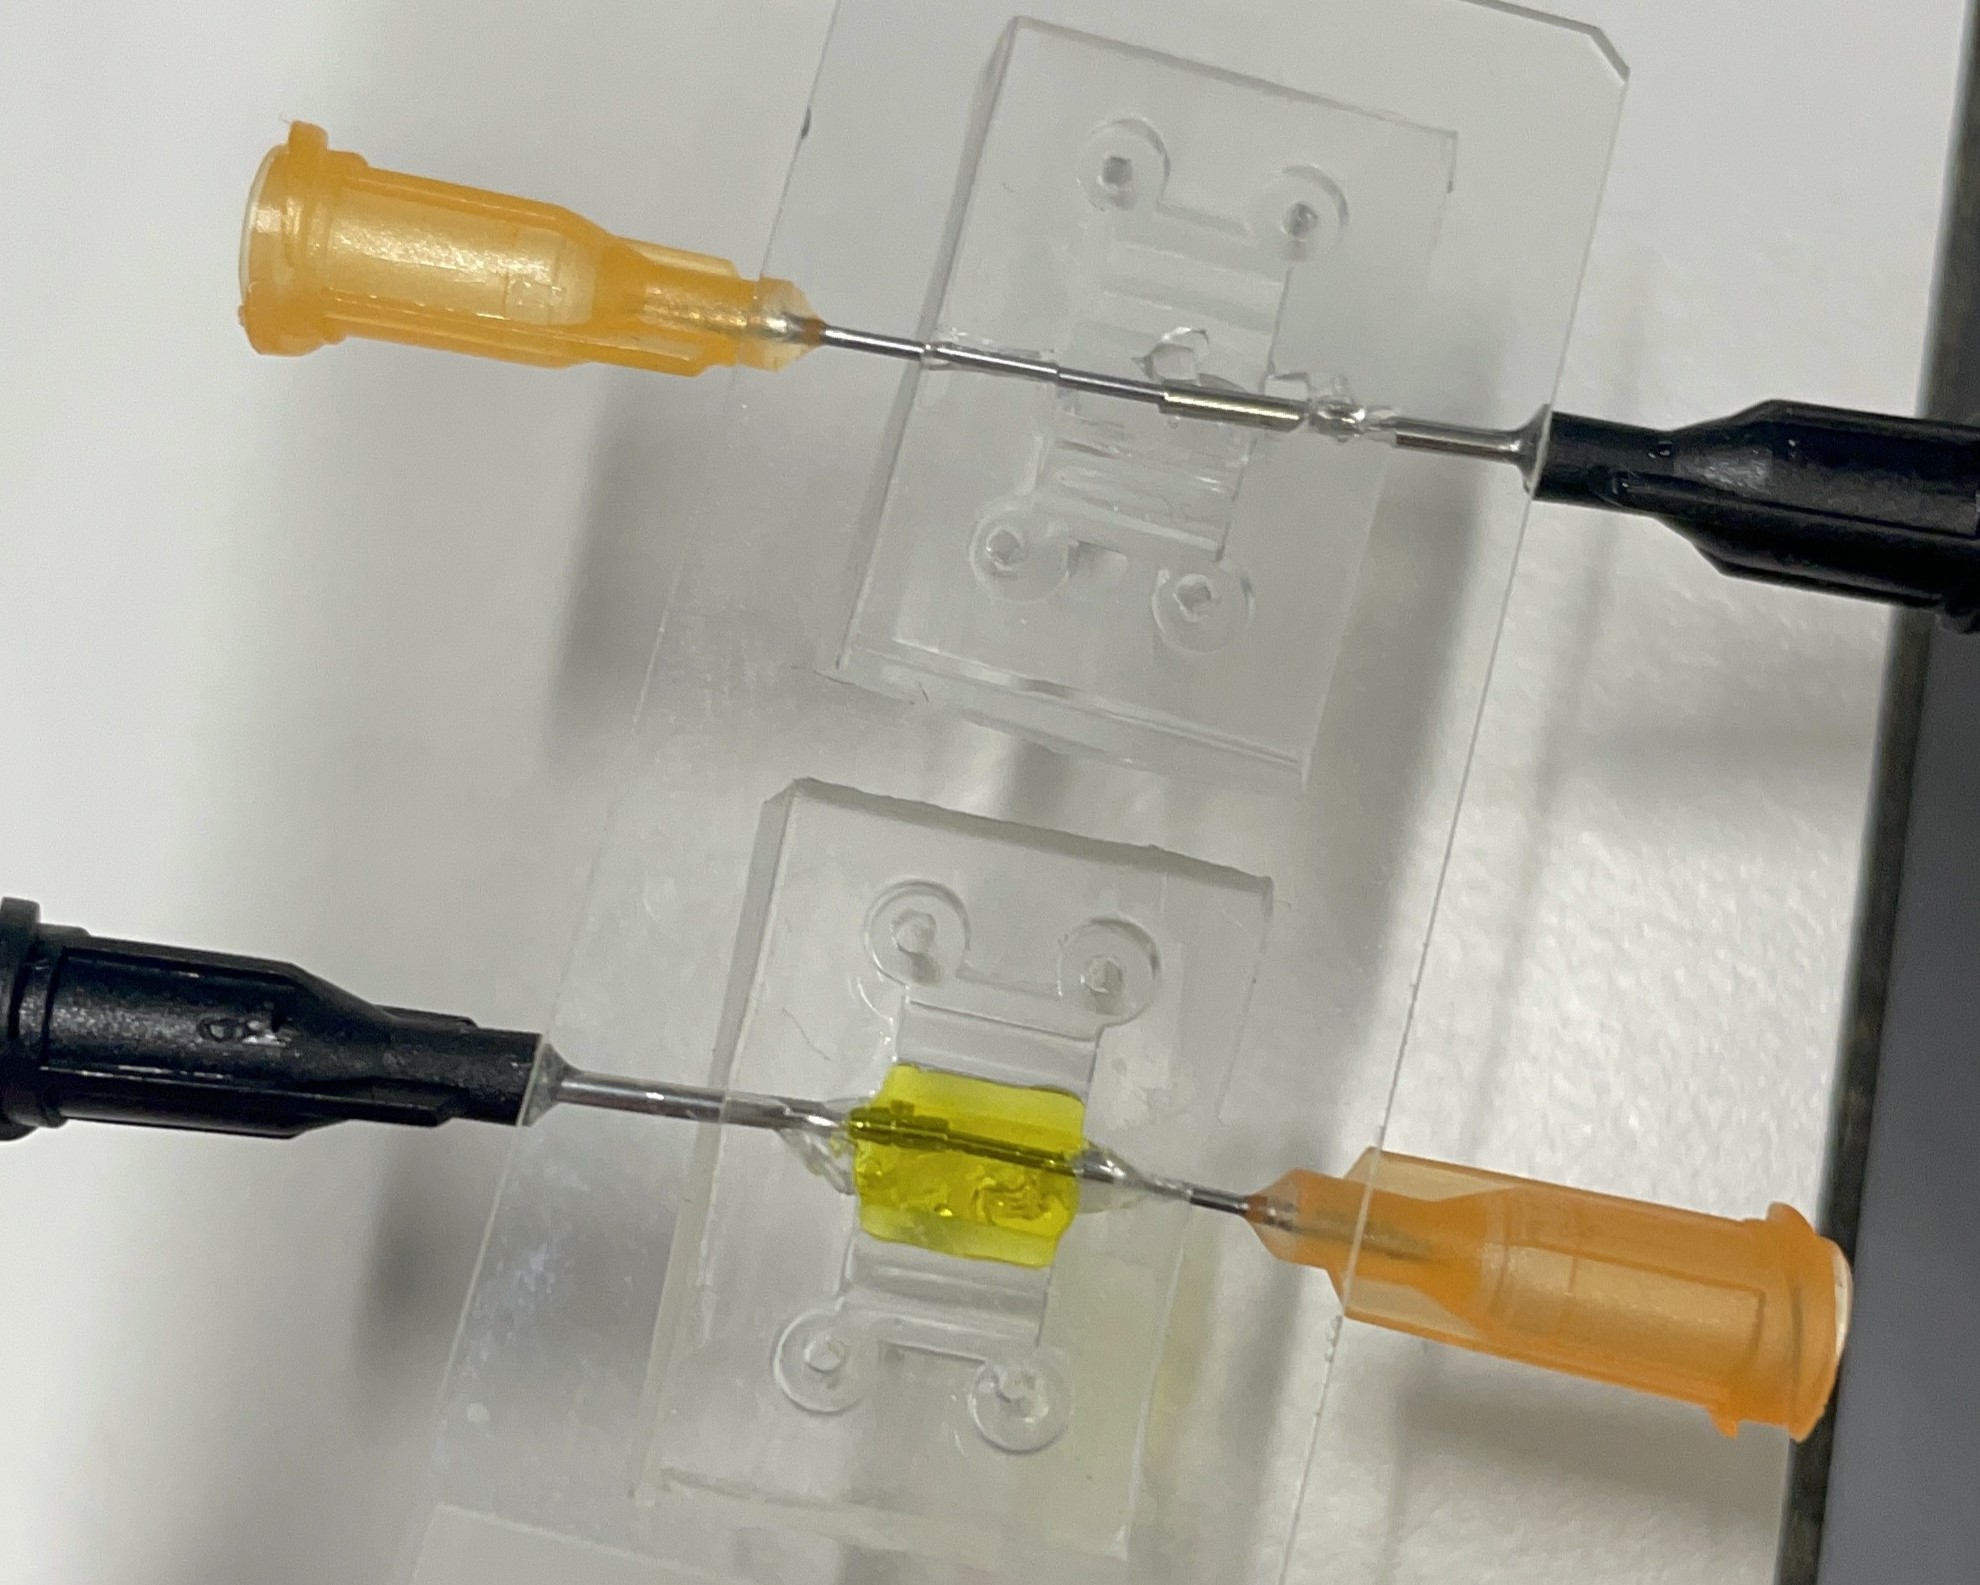
\includegraphics[width=0.75\linewidth]{dapp_report/figures/Fig W 5;4.jpeg}
    \caption{Hydrogel setting around needles in chips}
    \label{fig:W}
\end{figure}

In some chips, needles were removed, and a dyed fibrinogen/thrombin mixture was injected into the tunnel, to model the HUVEC culture. In other chips, three pipette tips were placed inside three of the four reservoir holes. Dyed water, as a model for growth media, was injected through the fourth hole with a filled pipette tip. The chips were then incubated at 37°C. 

These tests verify that the phase guides function correctly, stabilizing the hydrogel in the chamber without inhibiting fluid diffusion from the channels into the hydrogel. The chips were tested for visible leakage. The tunnel cast by the needles was visualized with the dyed mixture to determine its stability and shape. 

Both chips with and without hydrogel were tested for fluid diffusion. Without hydrogel, the test aims to verify the pressure gradients between the side channels.  With hydrogel, the test aims to verify that media can diffuse through the hydrogel, theoretically allowing nutrients to be provided and waste to be disposed of through pipette tip reservoirs. 

\subsubsection{Fluid flow results}

Fluid injection indicated that the hydrogel had correctly set and remained in place during the working of the chip; it was contained well by the phase guides, shown by the set yellow hydrogel (Figure \ref{fig:X}). Fluid flowed uninterrupted through the media channel and the media reservoirs (Figure \ref{fig:Y}). Fluid diffused well into the hydrogel and interacted with it without leakages (Figure \ref{fig:Z}). There was slow diffusion to the other side of the hydrogel and the waste channels. The chip features themselves showed no visible points of fluid leakage; however, in the chips that were not well adhered to the slides, small amounts of fluid leaked out. Filling the tunnel with dyed fibrinogen/thrombin mixture after removing the needles was difficult to control, but successful in some chips. The insertion of the two needles may have torn the PDMS slightly, given the messy line visualized by the tunnel cast in the hydrogel. 

\begin{figure}[h!]
    \centering
    \begin{minipage}[b]{0.3\linewidth}
        \centering
        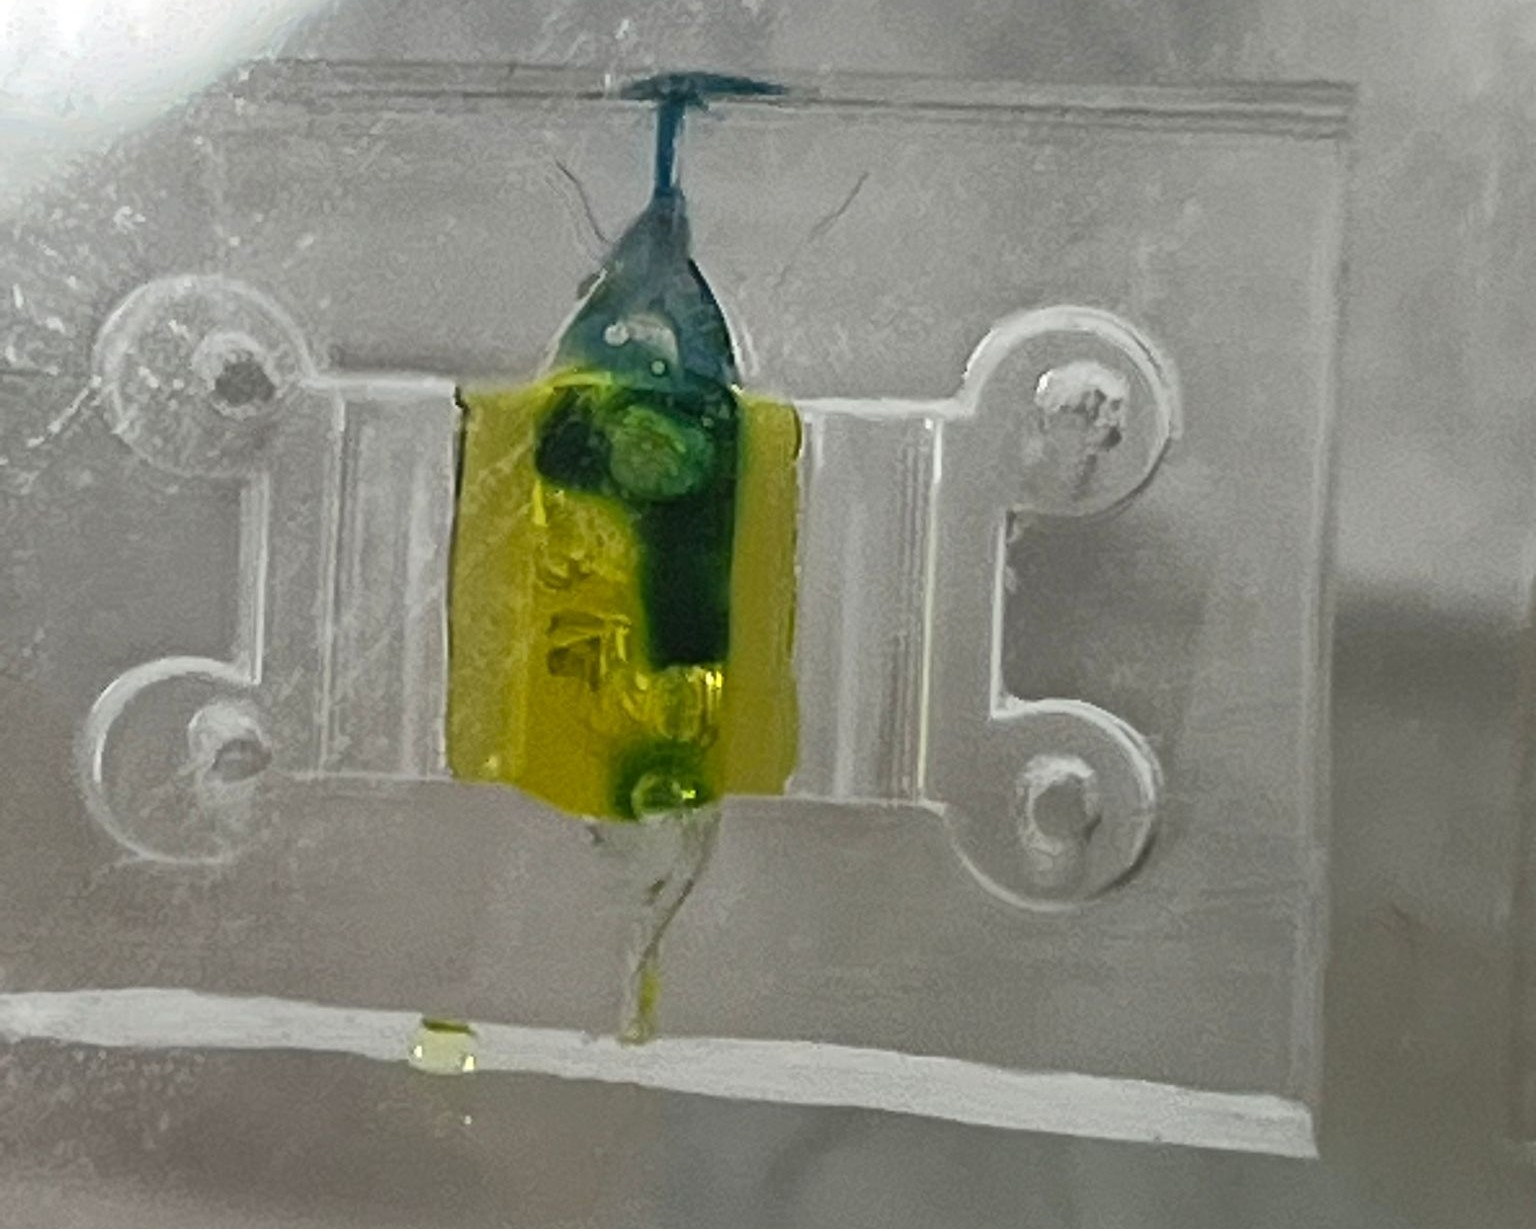
\includegraphics[width=\linewidth]{dapp_report/figures/Fig X 5;4.jpeg}
        \caption{Chip with injected hydrogel and extracted needle}
        \label{fig:X}
    \end{minipage}
    \hspace{0.03\linewidth}
    \begin{minipage}[t]{0.3\linewidth}
        \vspace{-4.6cm} % Adjust this value as needed
        \centering
        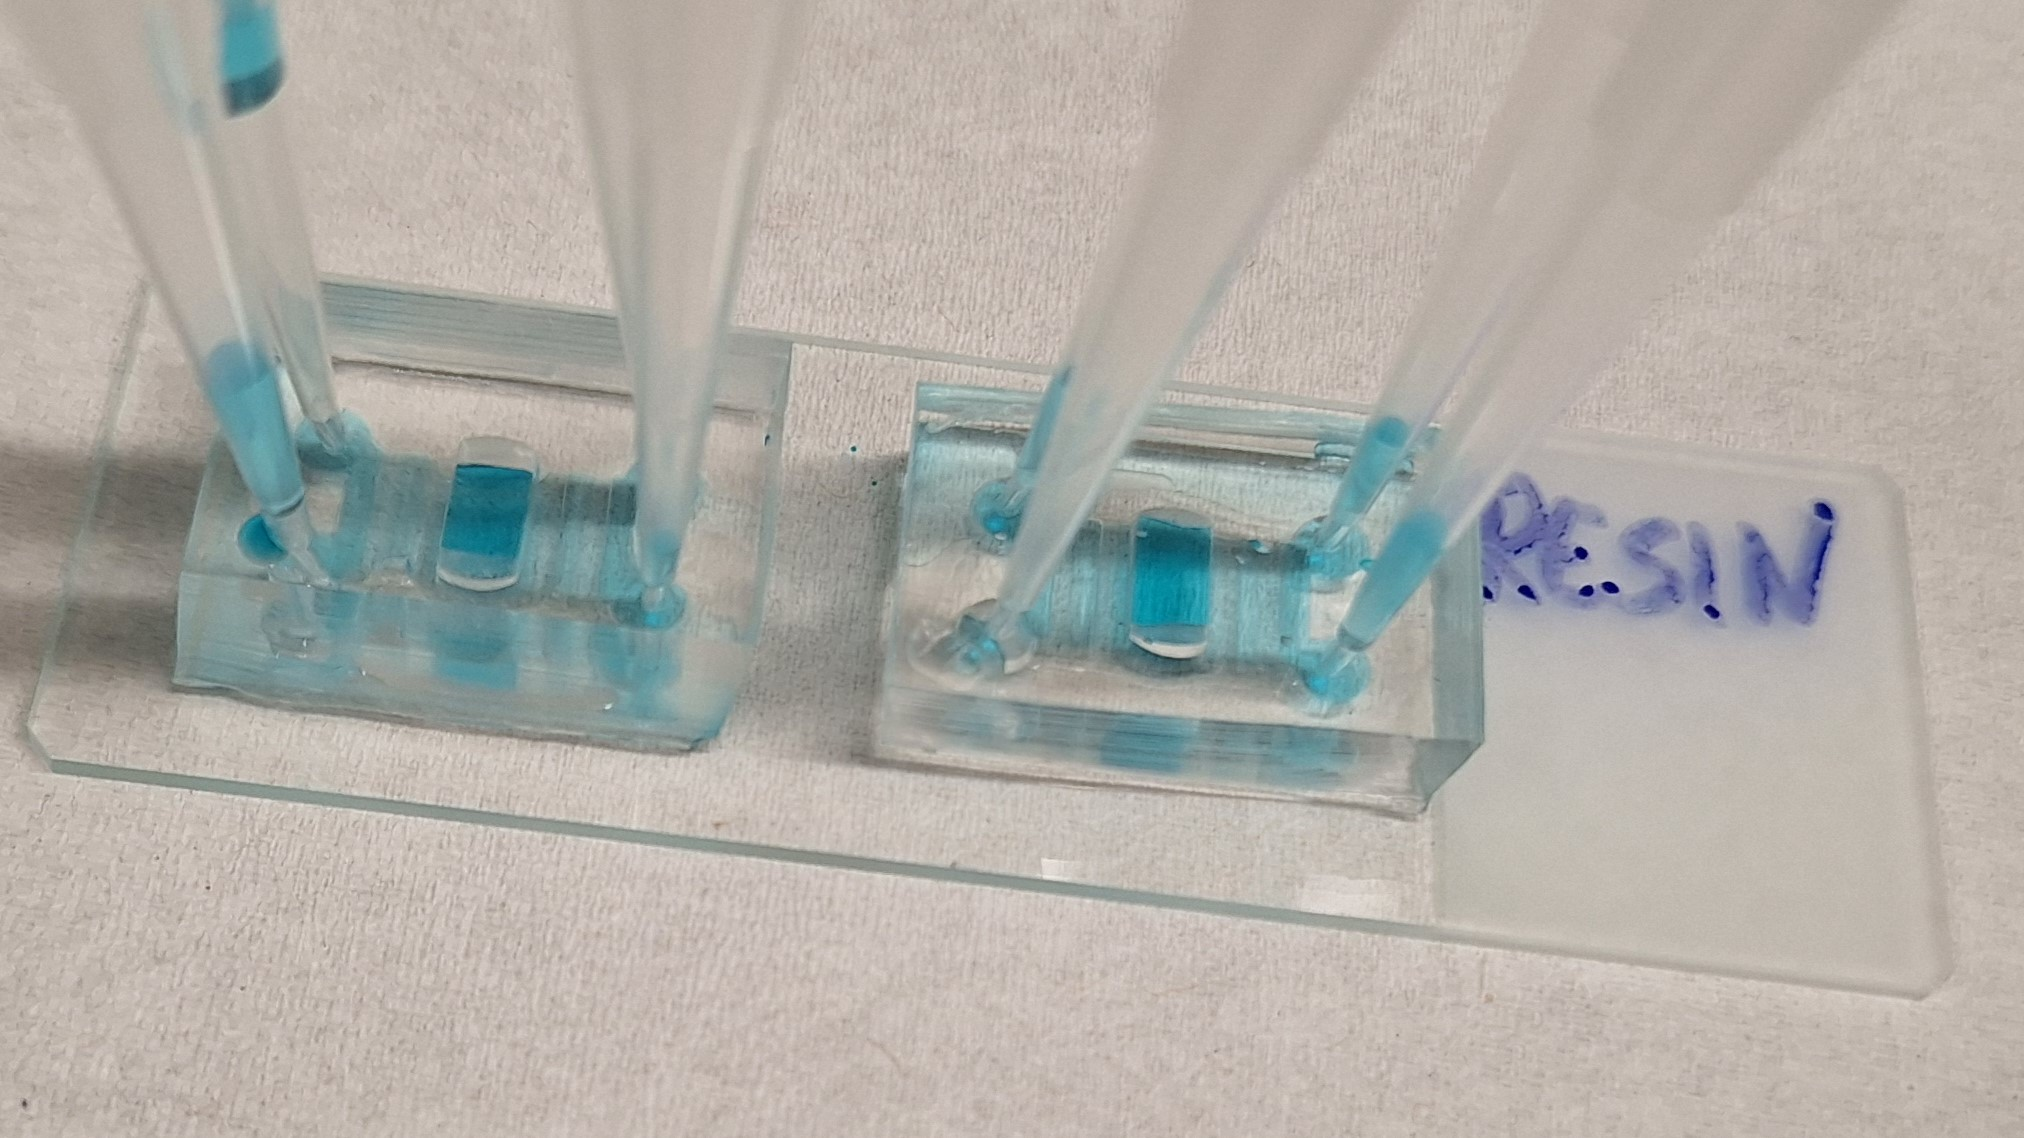
\includegraphics[width=\linewidth]{dapp_report/figures/Fig Y 16;9.jpg}
        \caption{Fluid flow test}
        \label{fig:Y}
    \end{minipage}
    \hspace{0.03\linewidth}
    \begin{minipage}[b]{0.3\linewidth}
        \centering
        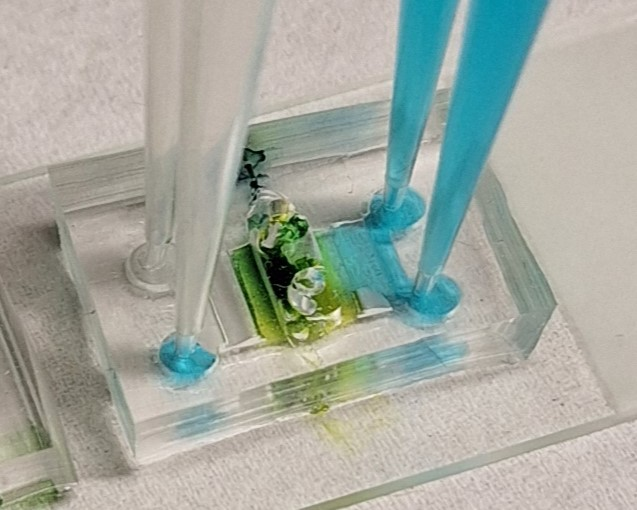
\includegraphics[width=\linewidth]{dapp_report/figures/Fig Z 5;4.jpg}
        \caption{Perfusion across hydrogel due to concentration gradient}
        \label{fig:Z}
    \end{minipage}
\end{figure}

\subsubsection{Fluid flow discussion}

The phase guides functioned as expected, and secondary phase guides were confirmed useful where primary phase guides proved insufficient. Given the successful diffusion of liquid from the side channels, it is expected that the growth factors will reach the cells in the central tunnel. 

Forming the tunnel in the hydrogel as a scaffold for the central feeder vessel proved difficult with one needle. It did not extend through the chamber length, so two needles were used instead. This modeled the injection of HUVECs and fluorescent dye into the hydrogel. The injection was relatively successful since the central tunnel formed correctly. However, the mixture did not permeate cleanly and fully through the tunnel. Needle insertion and removal caused slight tearing of the PDMS, therefore to simplify the technique, one longer needle should be procured instead. Future experiments could utilize a 0.625 mm biopsy punch to create an entry into the chip; this pierces the PDMS cleanly and provides a smooth entry for the needle. Gelation of the fibrinogen/thrombin mixture began within seconds throughout all experiments, so injections of this mixture, especially when in small volumes, must be done quickly. 





\subsection{Future Cell Culture Experiments}

Post injection of HUVECs, the chip will be inspected under 10x and 100x microscopy to verify vessel formation and check for contamination. Bright field imaging technique is chosen, as it provides the necessary resolution to observe the formation of the capillary network and is cost-efficient. Hoechst 33342, a DNA-binding dye, can be used during the imaging to examine the distribution of cells throughout the hydrogel. Permeability can be assessed by loading dextran dye into the tunnel. Capillary network continuity will be evaluated by filling the reservoirs with a phosphorescent fluid and observing the flow through the vessels. 



\subsection{Conclusion on discussion}
The current design iteration of the chip works relatively well. Some improvements in the manufacturing process include assessing the materials used to print the mould (resin is ideal for plasma bonding) and optimising the printing process so that the mould does not warp or adhere too strongly to PDMS. Further limitations primarily include the injection of the cells, and techniques involved in the experimentation - for example, the optimal method of injecting liquid into the central tunnel. 

Further testing is required to complete the full cell culturing protocol. Verification on a) whether the HUVECs can form the central feeder vessel in the tunnel created, b) whether the HUVECs can sprout through the hydrogel and create microvascular networks, and c) whether there are successful interactions and fluid flow of the injected growth factors and removal of waste products, is needed. Future experiments involve imaging the chip and cell cultures under a microscope to test visualisation ability and track the hypothesised growth of the cells. 


\subsection{Group dynamics and organisational improvements}
\subsubsection{Team organisation and task distribution}

Group work was carried out as a mixture of individual, sub-team, and whole-team events. Full team meetings were necessary for the cohesion of the project and to ensure all members were up to date. Further group sub-divisions proved more effective for achieving task objectives.  Increased sub-grouping allowed for further task specialisation, more fluid communication within smaller groups, and decreased clashes in availability. This is a format we would repeat in future projects.  

\subsubsection{Discussion format}

In-person meetings included more efficient and relevant discussion than online meetings, where large parts of the group would naturally take more passive roles. Online meetings were effective for sub-group communication or for meetings with our advisors.  

\subsubsection{Absences and meeting notes}

Our major organisational limitations in the project came about regarding communication within the group. An effort was made to take detailed notes during each meeting, which proved to be helpful to those not present or not in the subgroup to still be informed. These notes were most effective when they were highlighted, for example, in the group chat, and when it was ensured that everyone had read them. For maximal engagement in future projects, there would be more focus on creating these notes, and checking in with all members on whether they had any details to discuss. This increased lateral communication allows for more collaboration and inclusion between all group members, while allowing space for the subgroups to complete their tasks.   

\subsubsection{Theoretical phase and prototyping }

Often, it was the practical prototyping that revealed the most limitations, which then required significant changes, and a restart of the design process. The initial planning phase, which was fully theoretical, was a less efficient use of time. Manufacturing should have started earlier so we could become more aware more quickly of the practical errors. 

Although obvious in retrospect, internalising the transformation in strategy required applied work experience. Our future projects will rely on early and more extensive periods of prototyping, where multiple design alternatives will be investigated, before a final design is produced.   

\subsubsection{Summary } 

Overall, the team worked well together, and approached the project with both interest and academic commitment. While there were some communication and organisational issues, as outlined above, often these were resolved by each member’s dedication to the project. This made it easier to communicate issues when they did arise, and our reflection on the process showed the group where to focus and improve in the future. 

\newpage
\addcontentsline{toc}{section}{References}

\printbibliography[title=References]

\newpage


\section*{Appendices}

\appendix
\addappheadtotoc

\section{Project Management}
\subsection{Delegation of Duties}

The group leader, Povilas Sauciuvienas, was chosen by majority vote during the initial meeting of the group. His tasks included organising internal meetings, contacting supervisors, and arranging laboratory inductions and sessions. 
Under his leadership, weekly meetings were set up where the whole group discussed progress and distributed tasks. The frequency of these decreased during break periods and high load periods (i.e. exams) and increased before approaching deadlines.  
Further into the project, the group was divided into two subgroups to distribute the workload for increased efficiency. These divisions were as follows: 

\begin{itemize}
    \item \textbf{Chip design and Manufacturing}: This group was responsible for the design, manufacture, and printing of the moulds, PDMS chips, and the electromechanical elements associated with the slide rotator. The members included: Mir W. Tawshif, Henry J. A. Hollingworth, Shalini M. Sellam, Ming Zhu, and Povilas Sauciuvienas.
    \item \textbf{Hydrogel/Cells Group}: This group researched cells and executed hydrogel experiments, which included designing laboratory protocols, procuring appropriate cell dyes, and calculating the cost of the experiments. The members included: Jiayi Bai, Ruby Greer, Harsh Agrawal, Arman Asadi Moghaddam, Felix Syn, and Povilas Sauciuvienas\footnote{The group leader, while mainly active in the chip group, was added to both groups to monitor progress and communicate the necessary cross-group information.} 
\end{itemize}

Other specific delegated roles were as follows:
\begin{itemize}
    \item \textbf{Manufacturing leads}: Shalini M. Sellam and Mir W. Tawshif 
    \item \textbf{Finance lead}: Henry J. A. Hollingworth  
\end{itemize}

There were occasions when members of each subgroup would engage in cross-subgroup tasks where they were more knowledgeable about the matter.

During larger tasks, such as the Product Specification Document (PSD) and the final report, further divisions were made to allow the entire group to work on the task simultaneously. Each member took on responsibilities that best corresponded with their personal skills and role in the project.

\subsection{Research}
All team members were tasked with researching fields relevant to the project. Several research papers and resources on similar projects were identified, detailing the manufacture of microfluidic chips and the promotion of vascularization.

This research extended to more specific subjects such as factors affecting the vascularisation and angiogenesis of HUVECs and hydrogel properties. Subsequently, several proposals for the general design and direction of the project were put forward.  

\subsection{Design, Production, and Protocols}
Project progress was slowed down due to a prolonged theoretical phase, which involved many discussions to understand our aims and agree on the 'ideal' design. After the goal design was decided upon, the hydrogel group developed test protocols to be carried out later. Upon recognizing any errors or limitations, the design was improved. Multiple avenues were pursued simultaneously (e.g., simultaneously producing multiple moulds), and further procedures were built on the most promising results.

As such, the manufacturing team went through several design iterations. The earlier iterations of the mould and the PDMS were printed and cast respectively with assistance from PhD students, while the later mould iterations were printed by the team itself. Furthermore, five group members completed safety training in the CRUK microfabrication lab for PDMS casting and bonding. This training facilitated easier access to the PDMS station and expedited subsequent castings, which in turn increased the speed and efficiency of testing and redesigning the moulds. 

\subsection{Project Timeline}
% \ref{fig:gantt}

\begin{figure}[h!]
    \centering
    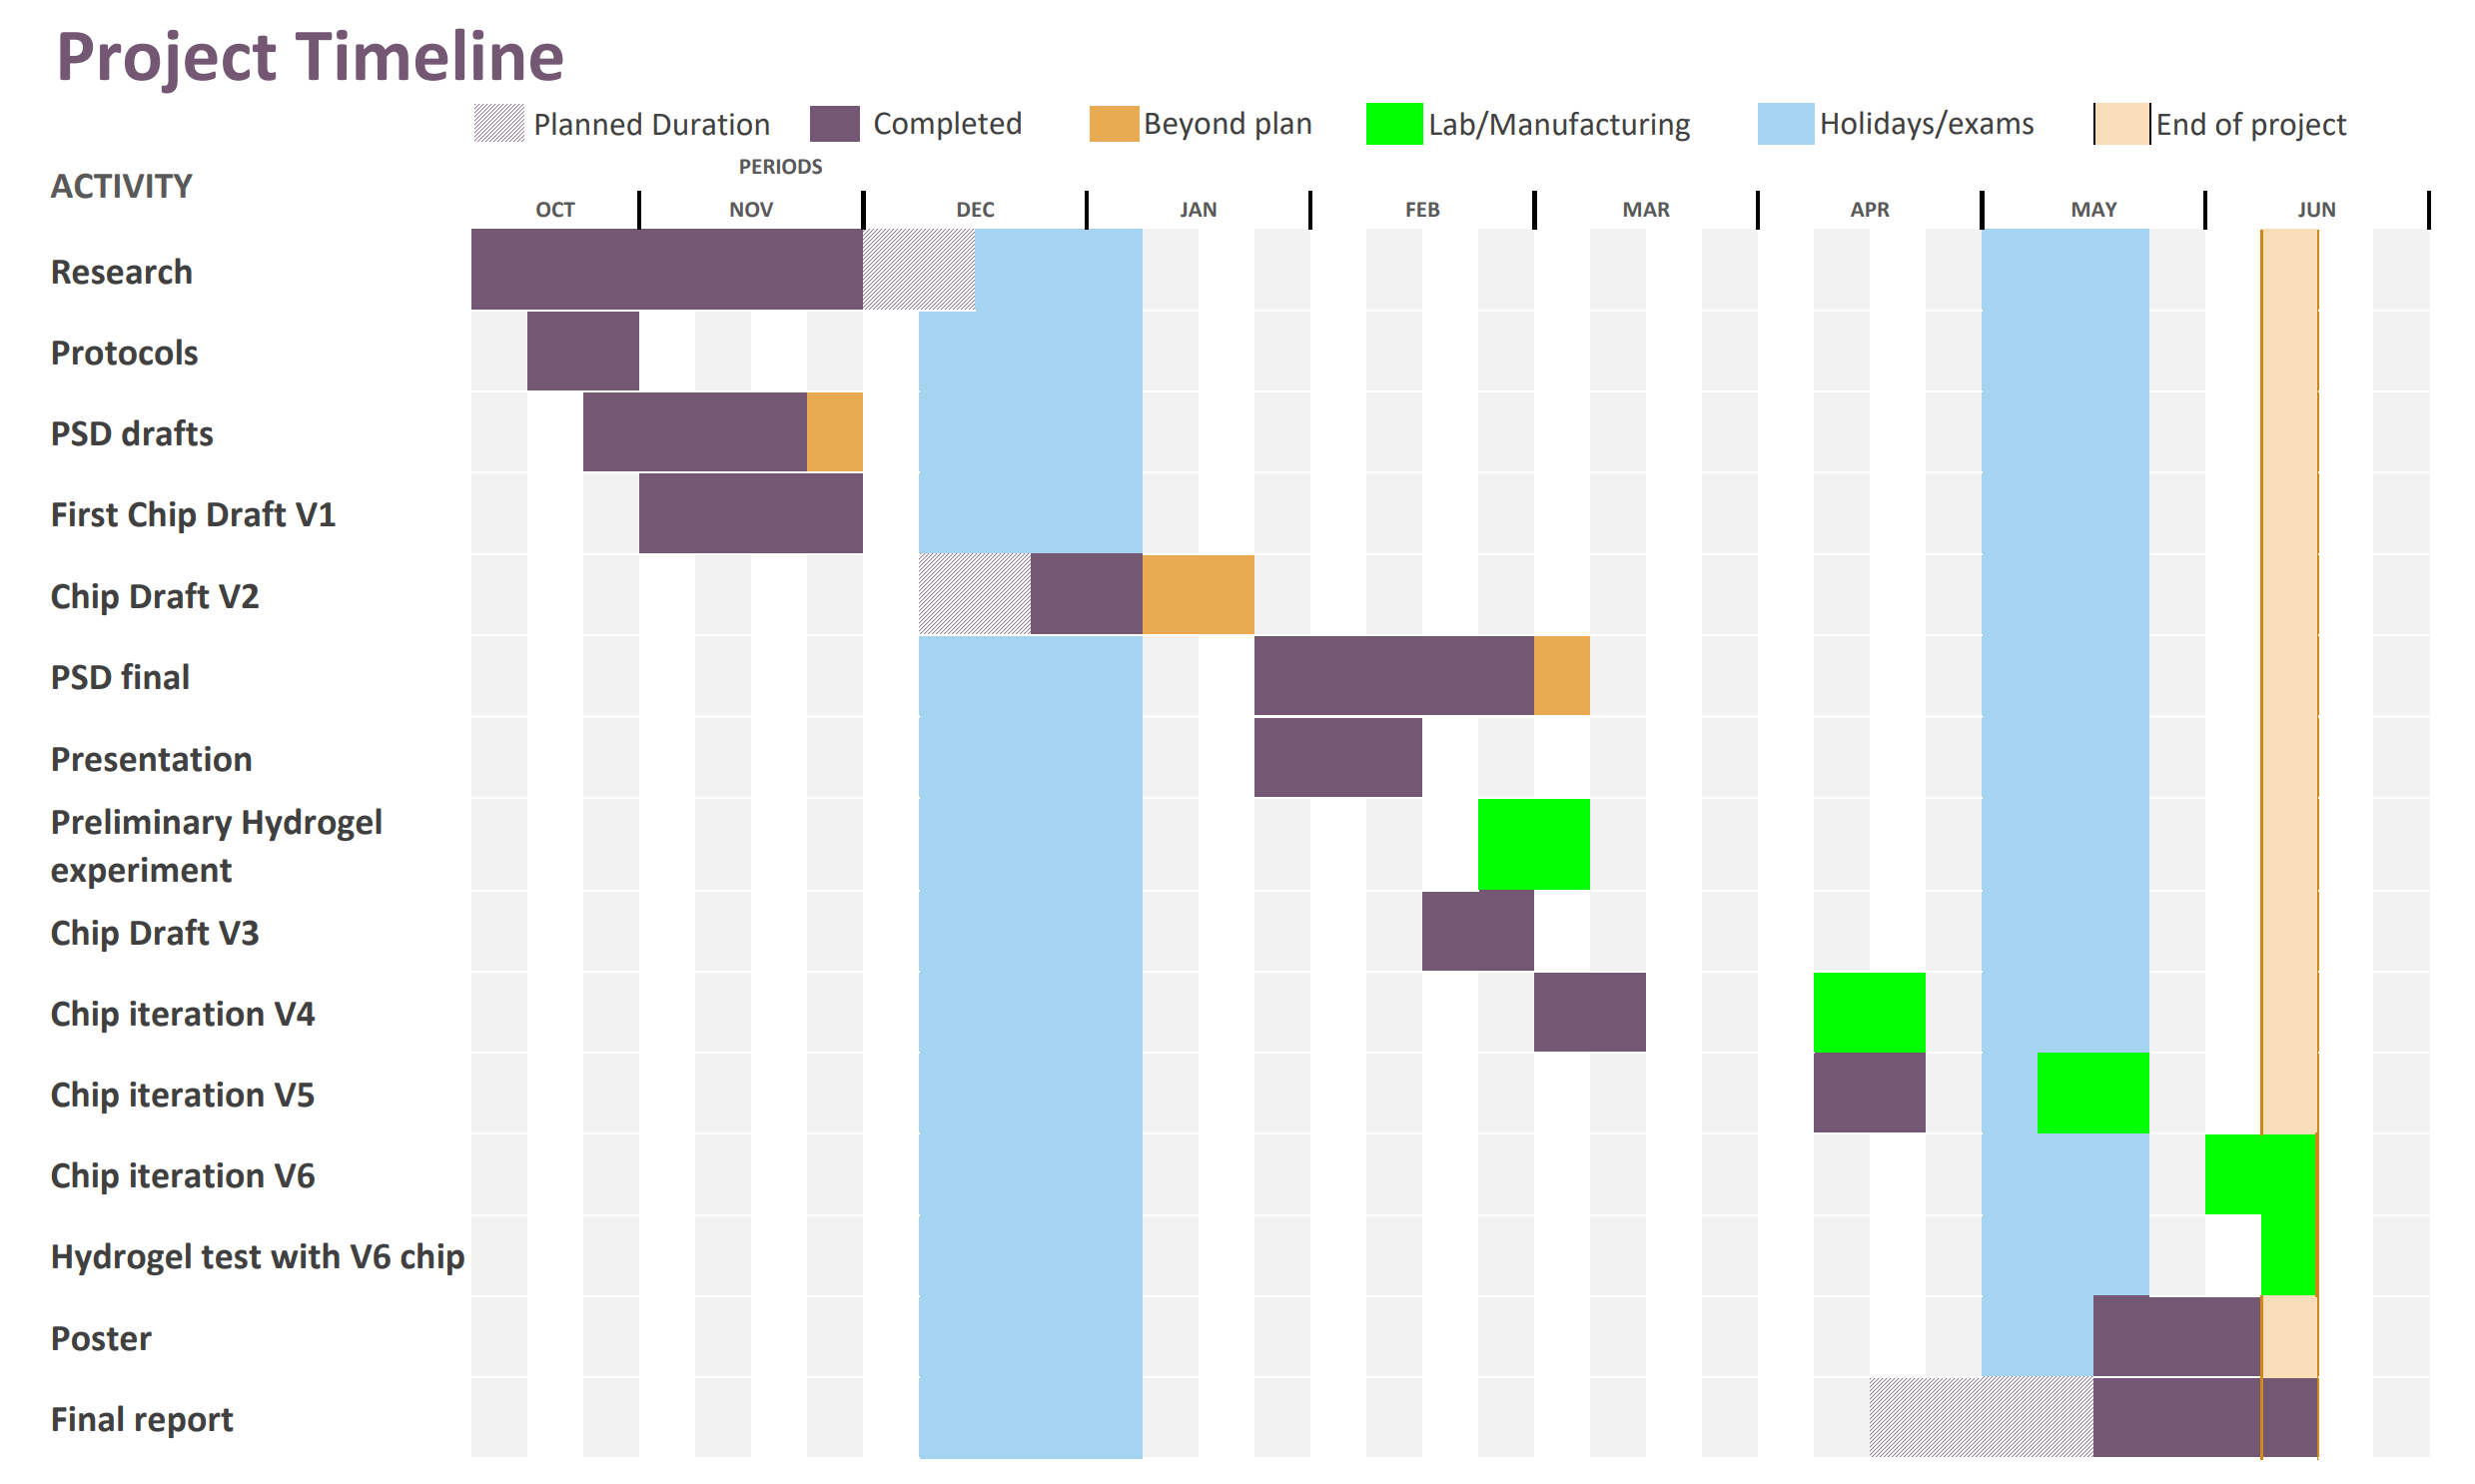
\includegraphics[width=1\linewidth]{figures/Gantt chart.png}
    \caption{Gantt chart showing progress along the during of the project.}
    \label{fig:gantt}
\end{figure}
\newpage

\section{Risk Management} \label{risk management}
Risk analysis for RPN threshold: 75\\
RPN = Severity (S) * probability of Occurrence (O) * Detection rate (D)
~
\begin{figure}[!h]
    \centering
    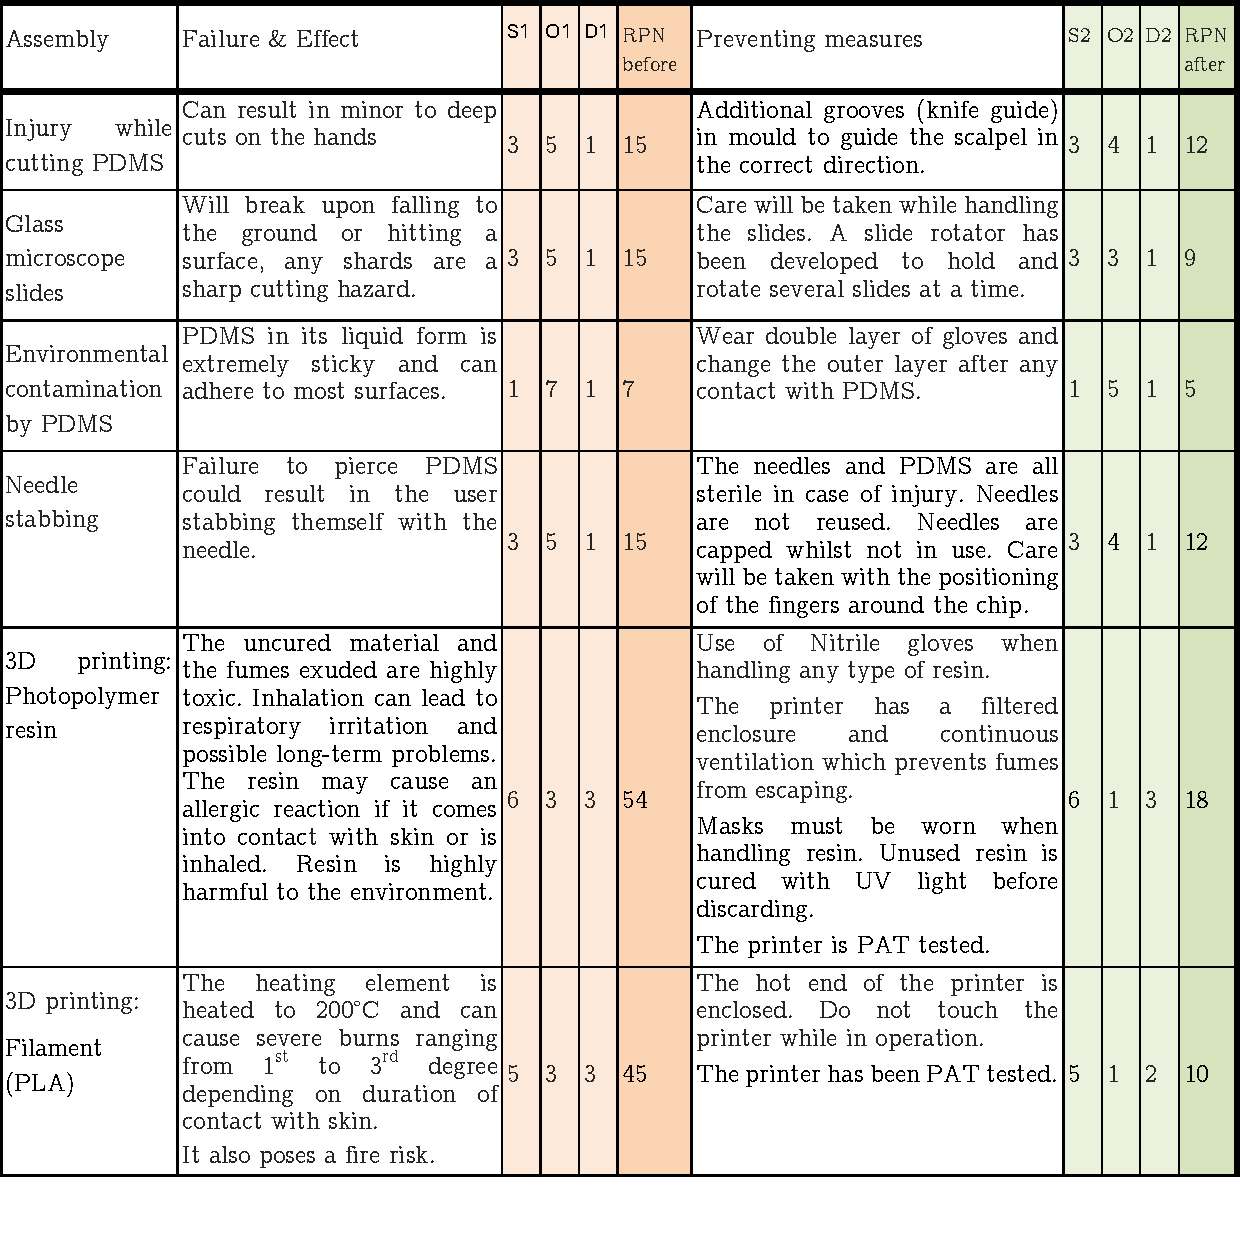
\includegraphics[width=1\linewidth]{PDF/our_risks.pdf}
    %\caption{Enter Caption}
    \label{fig:our_risks}
\end{figure}
 ~

\newpage

\section{Ethics} \label{ethics}


\subsection*{Respect for colleagues}

Meeting dates and times were determined by group votes based on common availability. During meetings, it was always ensured that everyone had a chance to express their opinions. If anyone had issues understanding the content of a discussion, other members demonstrated patience, and everyone made an effort to explain concepts clearly. Before tasks were assigned, each member’s preferences were recorded to ensure the optimal distribution of work.

\subsection*{Honesty, scientific integrity, and openness}

To ensure the validity of our project designs and results, all pertinent information about design progress and experiments has been thoroughly reported. This includes the limitations of our past and current designs, as well as all experimental issues encountered. All articles and designs that inspired our work or served as sources of information are appropriately cited as references throughout the report. Articles providing information that does not directly correspond to text within the final report are included in the bibliography. The technical drawing, which includes the dimensions of the chip, is provided for users, and both materials and working mechanisms are clearly listed.

\subsection*{Safety and Carefulness}

For laboratory experiments, the team consulted relevant experts, read, and strictly followed safety procedures to avoid harm to group members. Risks associated with the manufacture and use of the chip are analysed and appropriately mitigated in the risk analysis section. The manufacturing process was conducted following standard protocols to ensure the sterility of the chip. Each step was meticulously checked by group members to minimise errors that could propagate throughout the manufacturing process. All calculations were double-checked for accuracy.



\newpage



\section{Bill of Materials}

\begin{table}[!h]
\centering
\caption{Bill of materials}
\label{tab:bill}
\begin{tabular}{|m{4cm} |m{5.5cm} |m{1.8cm} |m{1.5cm} |m{1cm} |m{1.2cm}|} \hline 

\textbf{Material} & \textbf{Description} & \textbf{Supplier} & \textbf{Unit cost (GBP)} & \textbf{QTY} & \textbf{Total cost (GBP)} \\ \hline  \hline 

Resin, 500ml bottle & Material of mould & Amazon & 16.99/U & 1 & 16.99 \\ \hline 

Thrombin & The enzyme converts fibrinogen to fibrin & Sigma Aldrich & 322/U & 0.05 & 16.1 \\ \hline 

Fibrinogen (bovine) & Basic component of hydrogel & Sigma Aldrich & 238/g & 0.1 & 23.8 \\ \hline 

Hoechst 33342, 50ml vial & DNA-binding dye to examine distribution of cells & Cambridge Bioscience & 111.6/U & 1 & 111.6 \\ \hline 

32G Needle/ 100 pack & Creating space for feeder vessels growth & Amazon & 24.98/U & 1 & 24.98 \\ \hline 
Isopropyl alcohol & Eliminate any unexposed resin and enhance the sharpness of the printed features & Amazon & 7.95/L & 1 & 7.95 \\ \hline 

White PLA 3D printer filament & For prototyping of slide rotator & Amazon & 15.99/kg & 1 & 15.99 \\ \hline 
Arduino Nano 33 IoT & For prototyping of slide rotator & Imperial College London & 23.4/U & 1 & 23.4 \\ \hline 
12V power supply & For prototyping of slide rotator & eBay & 8.99/U& 1 & 8.99\\ \hline 
L298N Dual H Bridge Stepper Motor Driver Controller Board & For prototyping of slide rotator & eBay & 4.9/U & 1 & 4.9 \\ \hline 
12V connectors/ 5 pack & For prototyping of slide rotator & eBay & 3.59/U & 1 & 3.59 \\ \hline 
PDMS station & PDMS casting (includes the cost of PDMS and use of tools) & Imperial College London & 15/h & 7 & 105 \\ \hline 
Plasma treatment & Treatment station for Bonding PDMS and Slides & Imperial College London & 10/h & 3 & 30 \\ \hline 

Food dyes & Dyes to test the functionality of the vessel network. & Imperial College London & N/A  & N/A & N/A \\ \hline 
\hline 
 & &   \multicolumn{3}{c}{Grand total of 394.29 GBP} &  \\ \hline

\end{tabular}
\end{table}





\newpage

\section{Previous Chip Design Iterations} \label{app_chip_evolution}

% \ref{fig:TDV1}
\subsection{Chip v1}
\begin{figure}[!h]
    \centering
    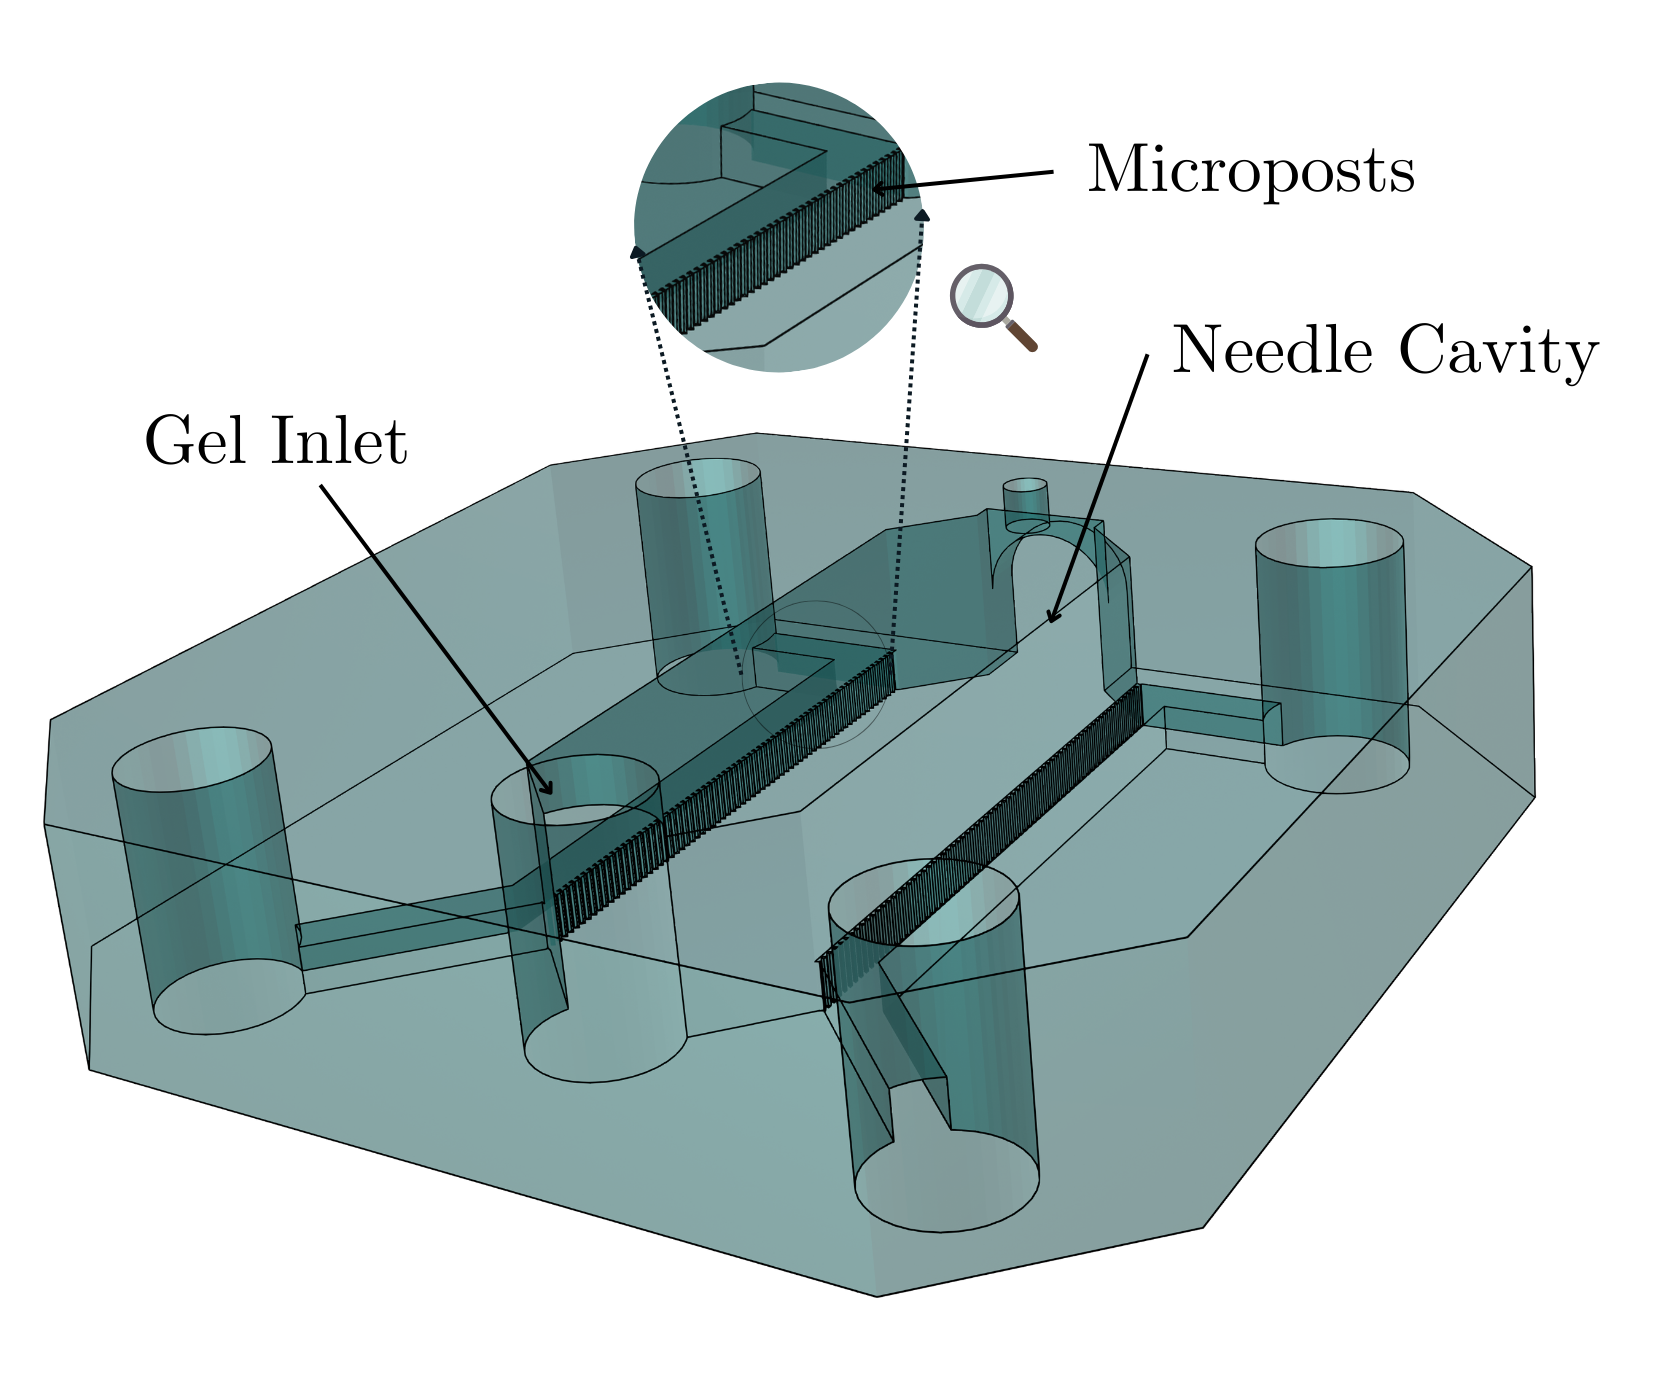
\includegraphics[width=0.8\linewidth]{dapp_report/figures/first_iter.png}
    \label{fig:first_iter}
    \caption{Annotated graphic of the first design iteration displaying important features.}
\end{figure}

\textbf{Features}: Microposts were the central feature of this design. Their compact spacing not only confines the hydrogel mixture to the central channel but also allows the media in both side channels to physically interact with the solidified hydrogel. The gel inlet is the point where the liquid hydrogel mixture is injected, and a small outlet on the other side of the central chamber allows air to exit. This setup results in the hydrogel being leveled as it solidifies. The needle cavity size was designed to fit a needle attachment to the chip, stabilising its position. Additionally, the length of the central channel was longer than that of the needle.

\textbf{Problems}: The negative moulds of microposts failed to print due to the x-y resolution limits of MSLA 3D printers. Air bubbles formed in the hydrogel when the needle was purged, which tore the set hydrogel. Additionally, the needle cavity posed a problem due to hydrogel leakage. 

\begin{figure}[!h]
    \centering
    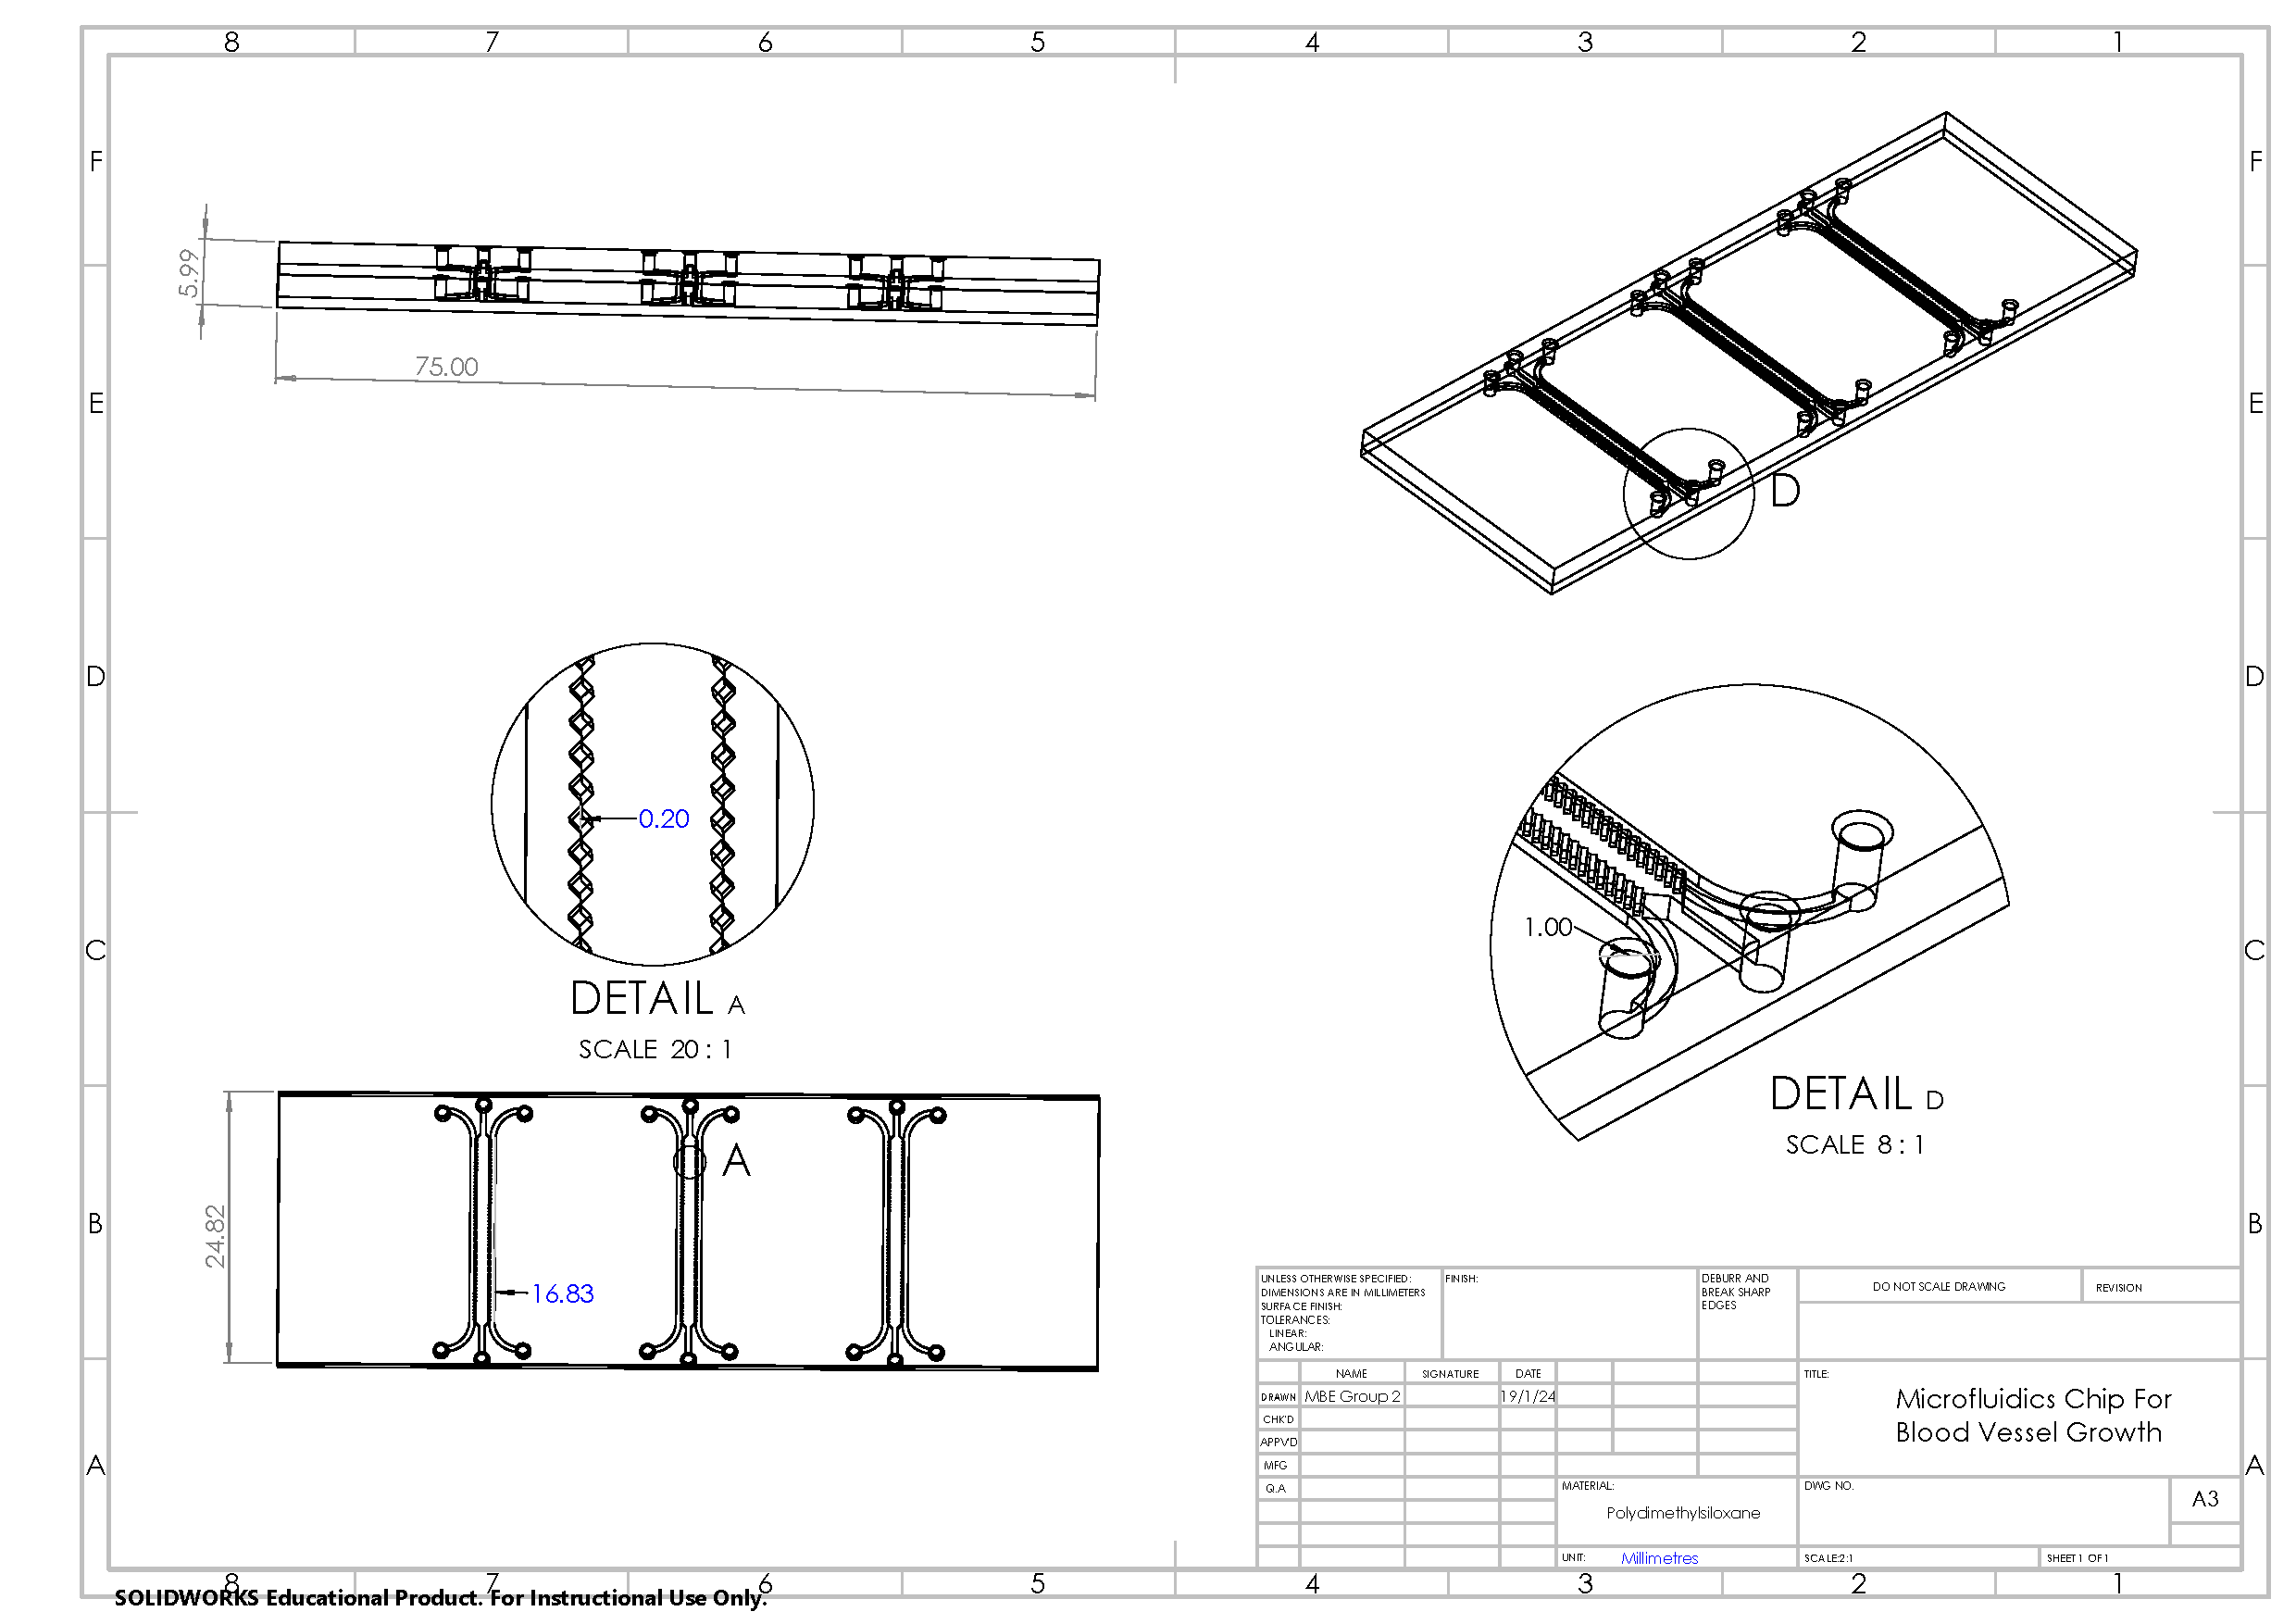
\includegraphics[width=1\linewidth]{PDF/TDV1.pdf}
    \caption{Technical Drawing of the first design iteration.}
    \label{fig:TDV1}
\end{figure}

\clearpage

\subsection{Chip v2}
\begin{figure}[!h]
    \centering
    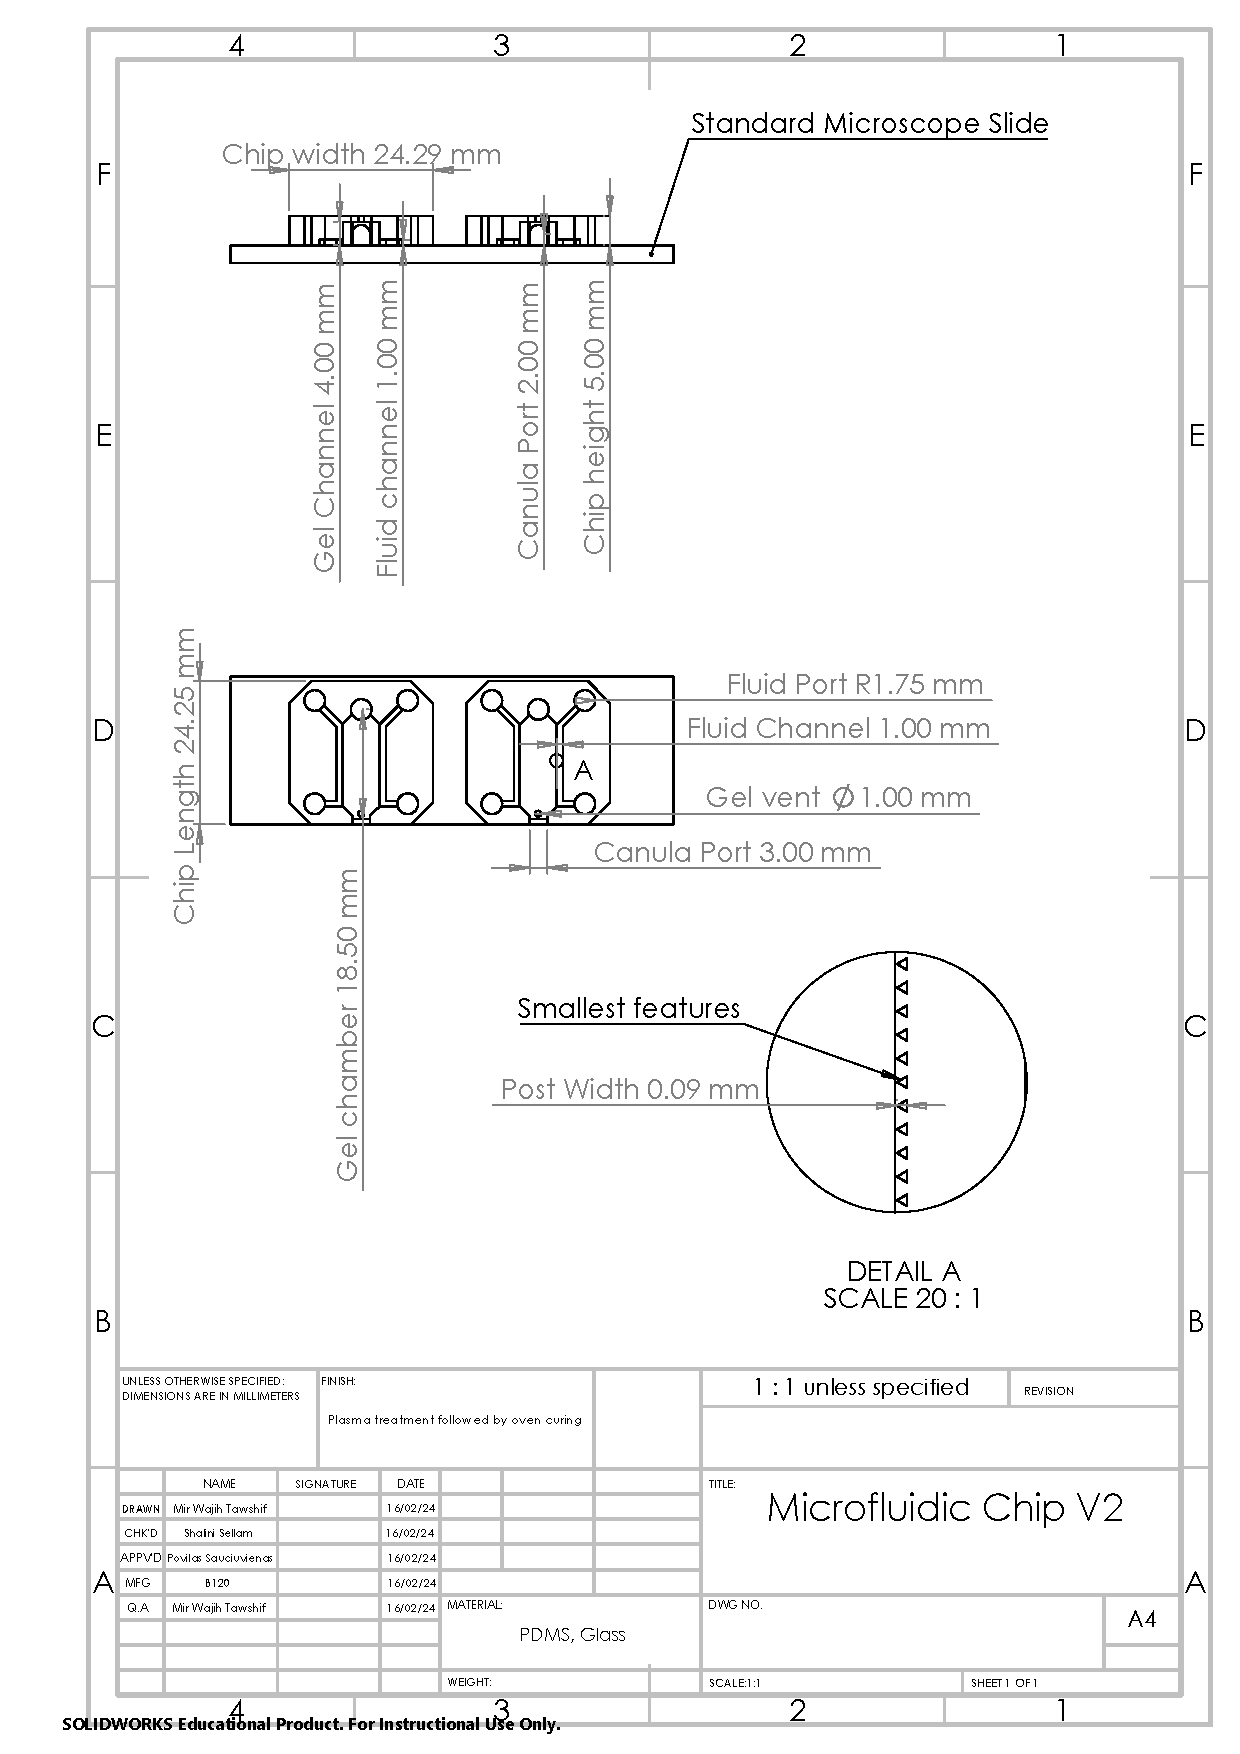
\includegraphics[width=0.8\linewidth]{PDF/TDV2.pdf}
    \caption{Technical Drawing of the second design iteration.}
    \label{fig:TDV2}
\end{figure}

\clearpage

\subsection{Chip v3}
\begin{figure}[!h]
    \centering
    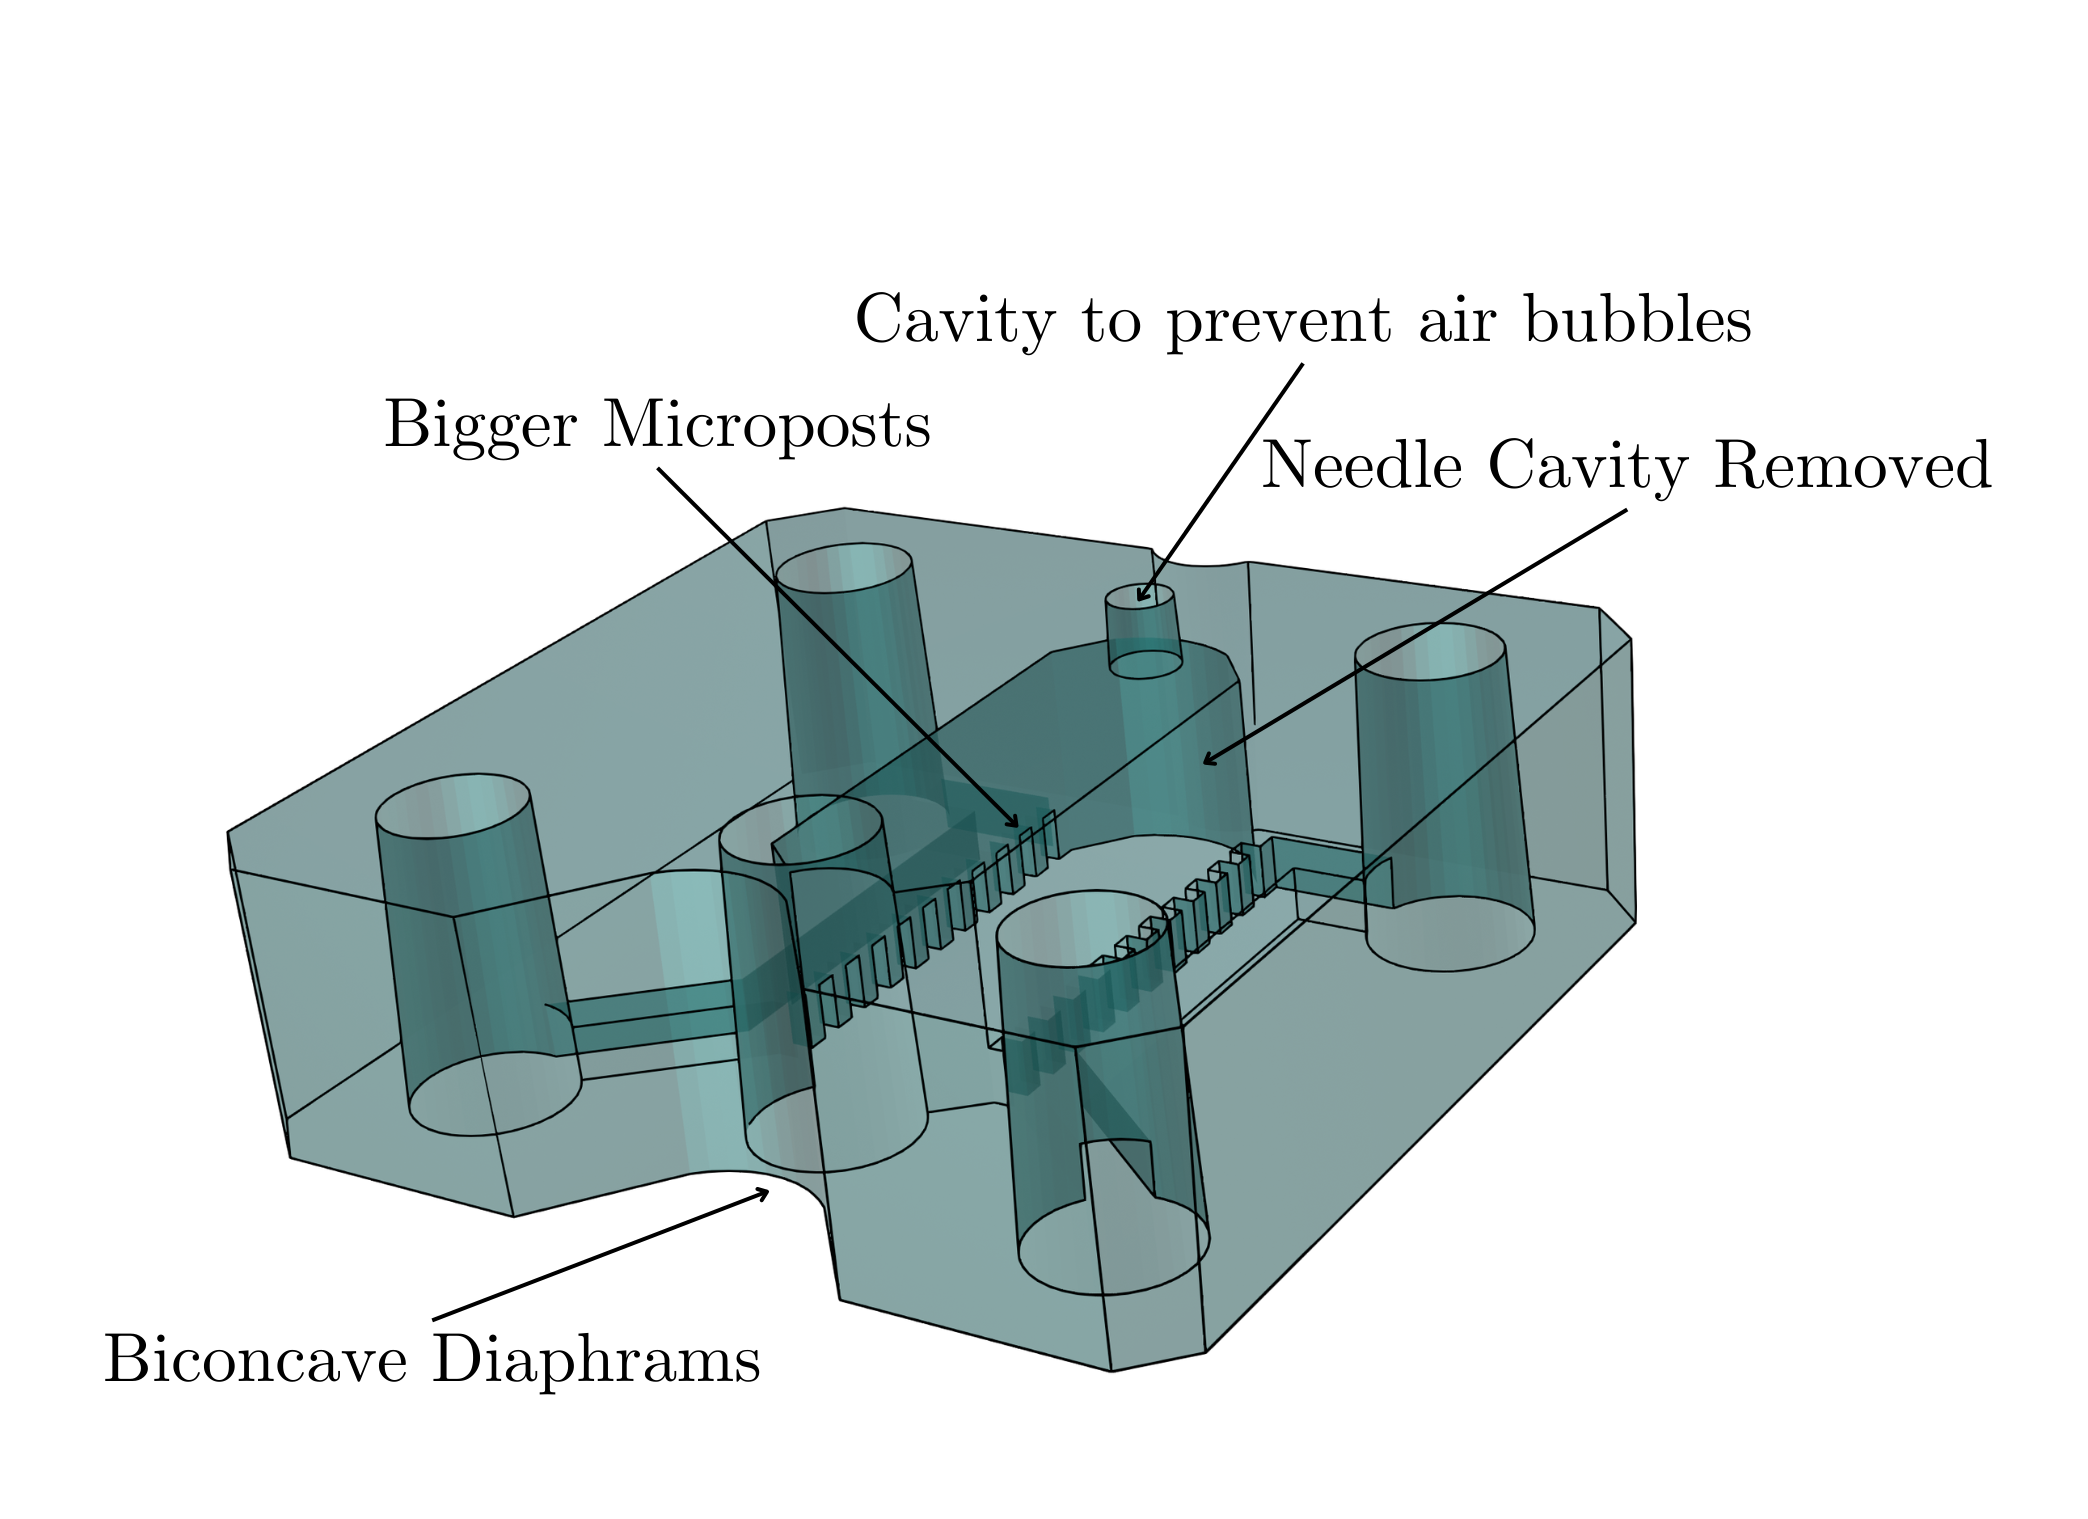
\includegraphics[width=1\linewidth]{dapp_report/figures/second_iter.png}
    \label{fig:second_iter}
    \caption{Annotated graphic of the second design iteration displaying important features.}
\end{figure}

\textbf{Features}: Microposts were enlarged to enhance printing success. The length of the central channel was reduced to be shorter than the needle to facilitate air purging from the needle. The needle cavity was replaced with a biconcave diaphragm, capitalising on the flexibility of PDMS, which allows it to be pierced while still maintaining a seal around the needle.

\textbf{Problems}: Despite these changes, the micropost negative moulds still failed to print due to the x-y resolution limits of MSLA 3D printers.


\begin{figure}[!h]
    \centering
    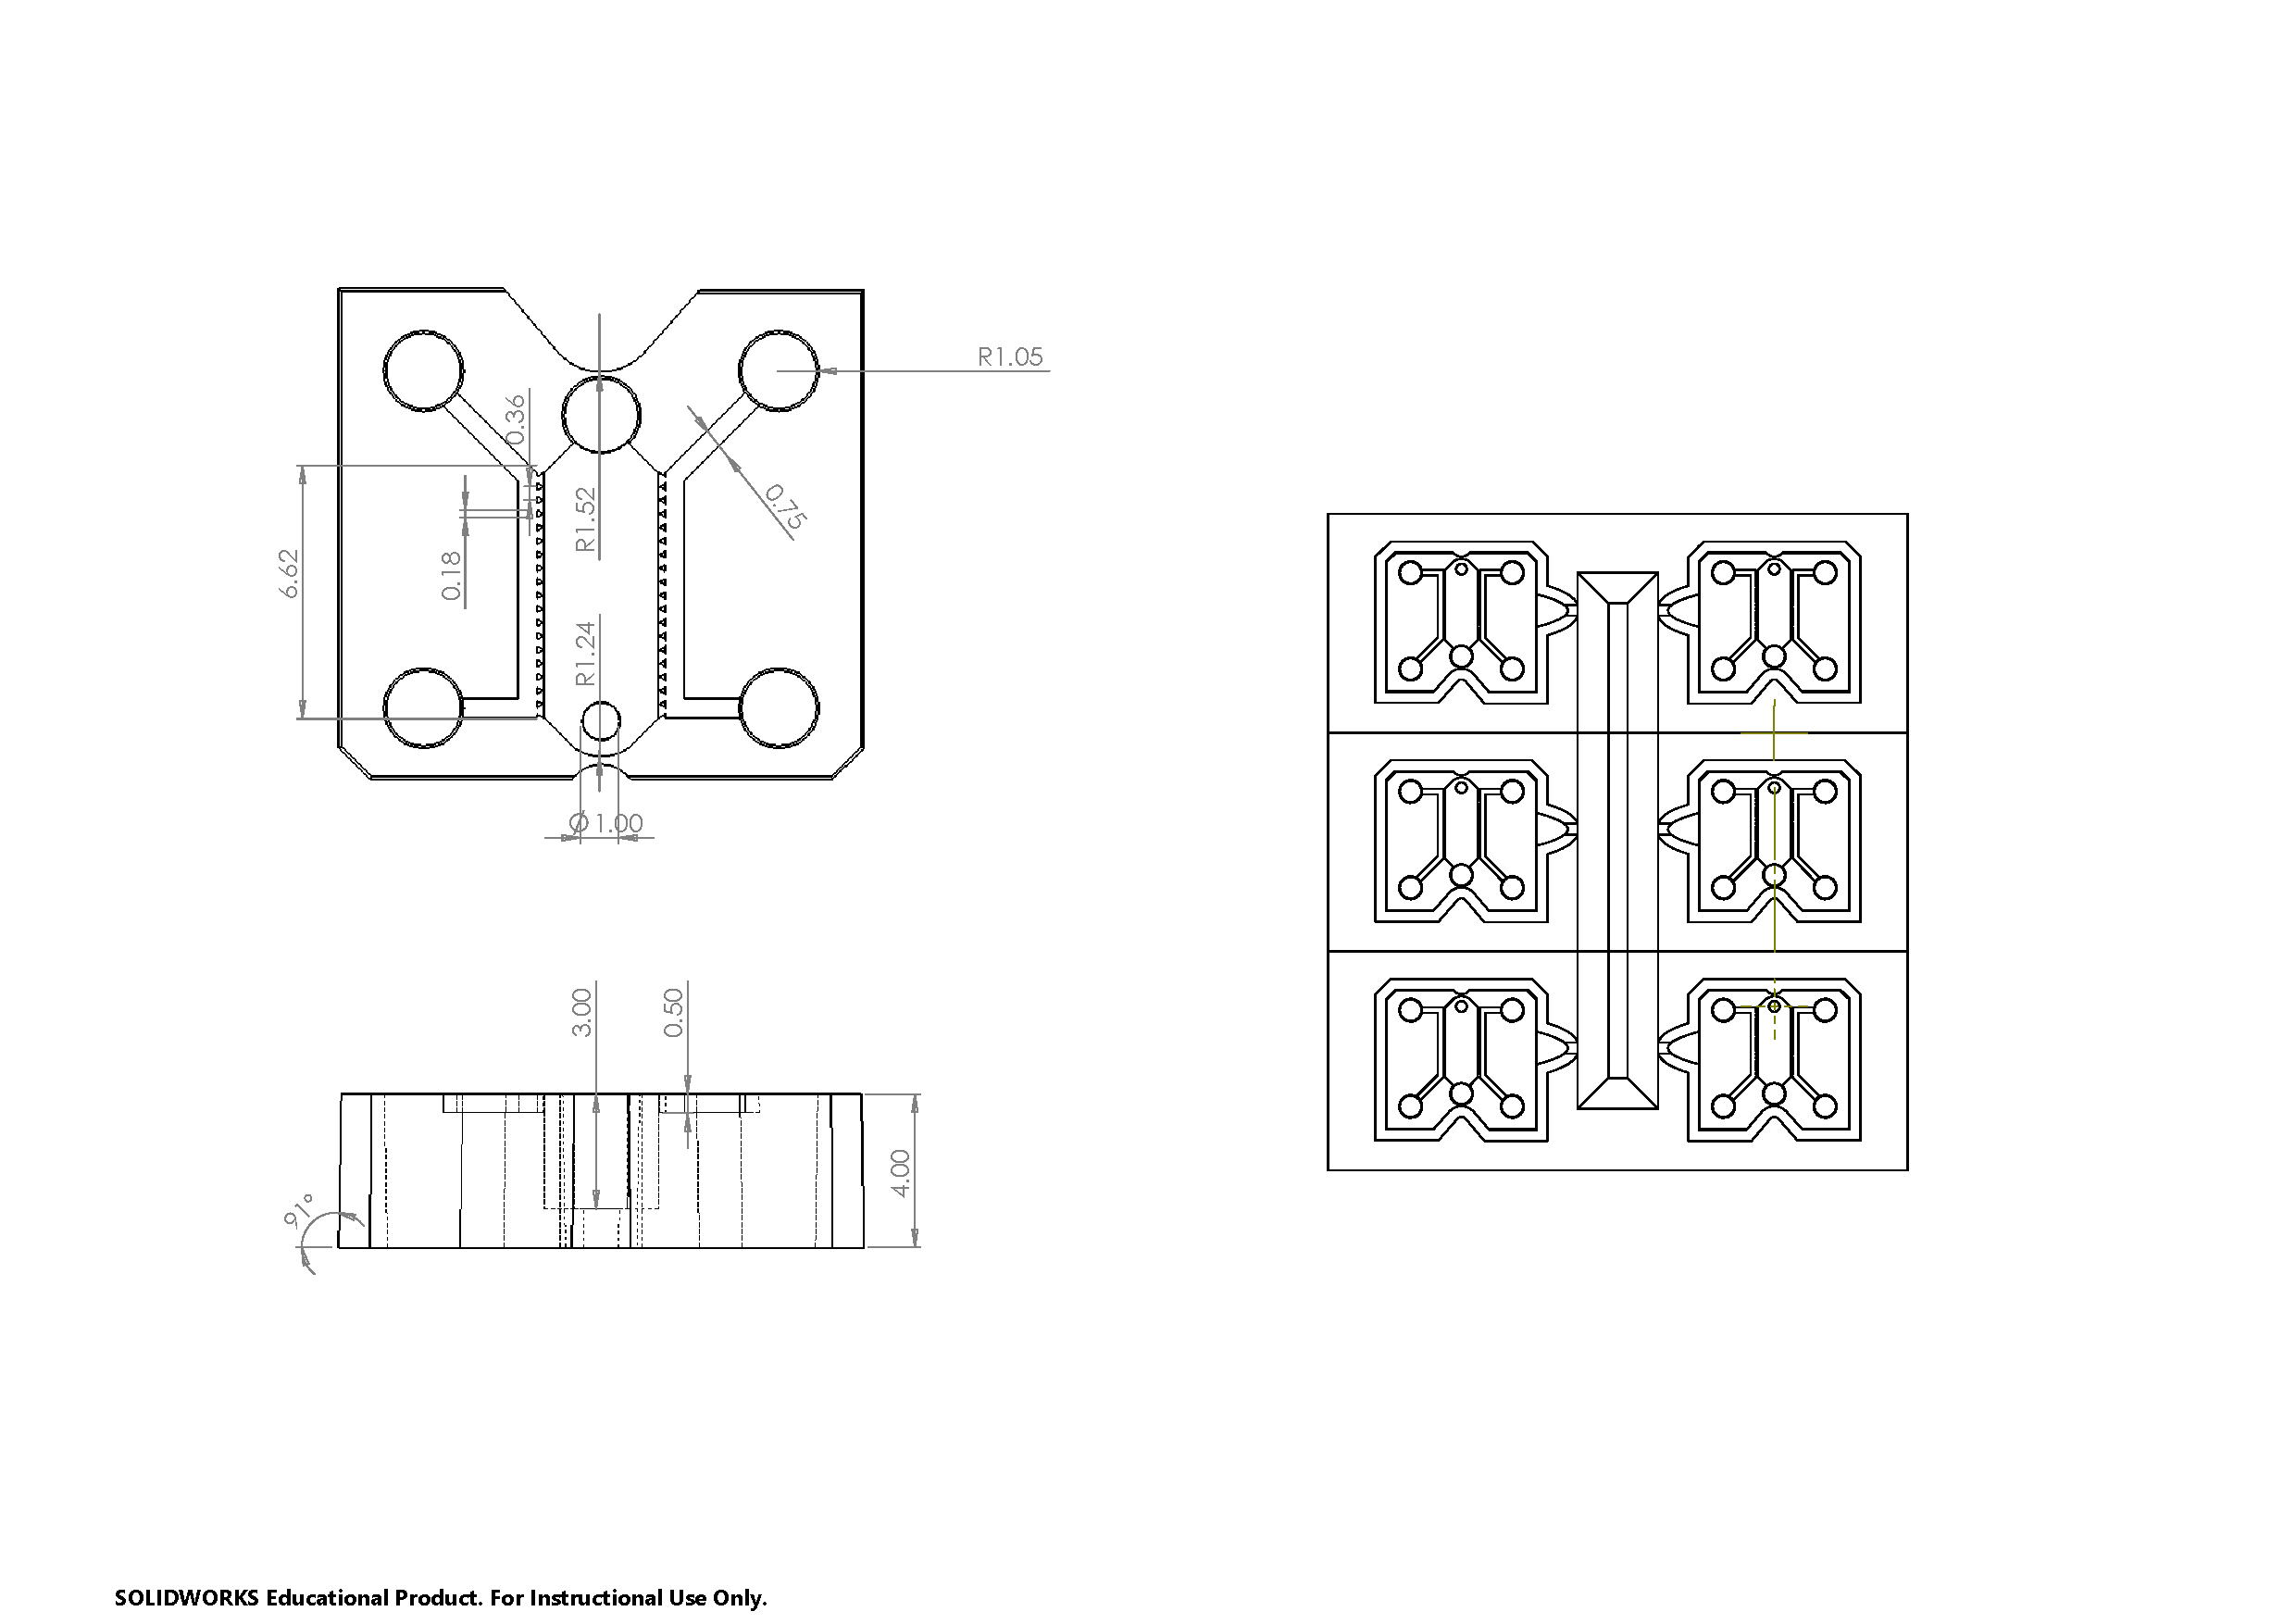
\includegraphics[width=1\linewidth]{PDF/TDV3.pdf}
    \caption{Technical Drawing of the third design iteration.}
    \label{fig:enter-label}
\end{figure}

\clearpage
\subsection{Chip v4}
% \vspace*{\fill}
\begin{figure}[!h]
    \centering
    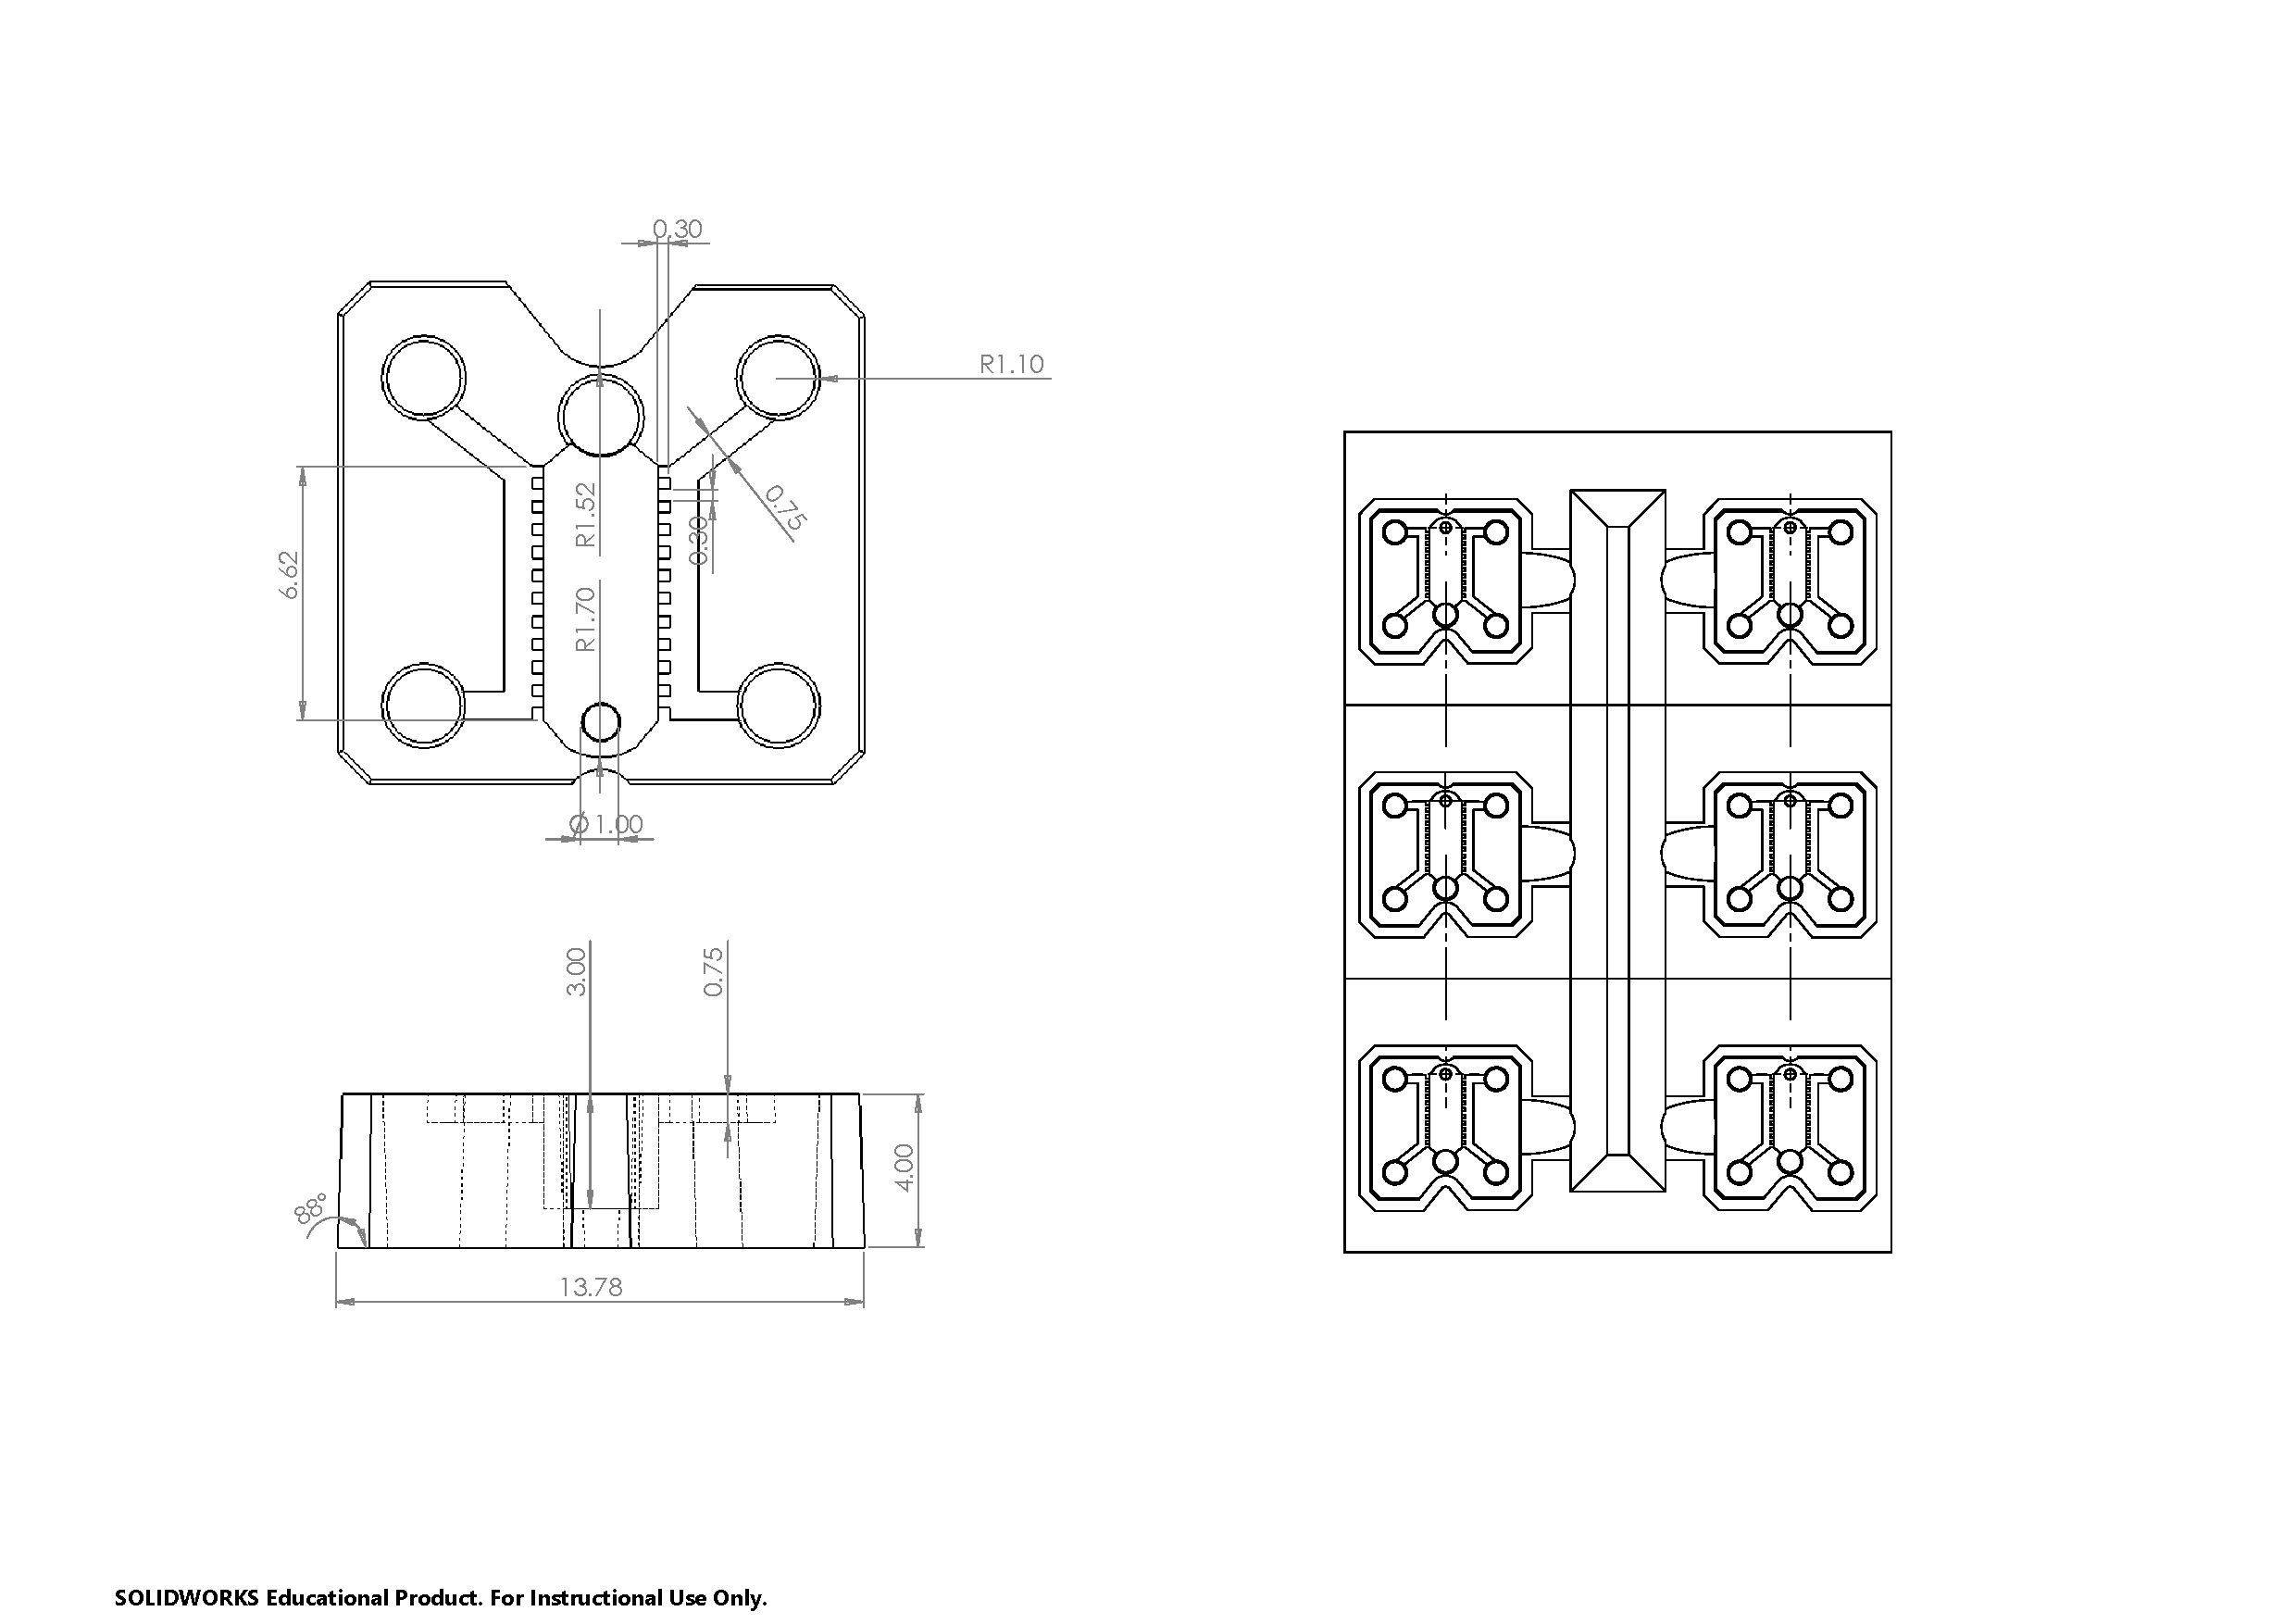
\includegraphics[width=1\linewidth]{PDF/TDV4.pdf}
    \caption{Technical Drawing of the fourth design iteration.}
    \label{fig:TDV4}
\end{figure}
% \vspace*{\fill}
\newpage

\subsection{Chip v5}
\begin{figure}[!h]
    \centering
    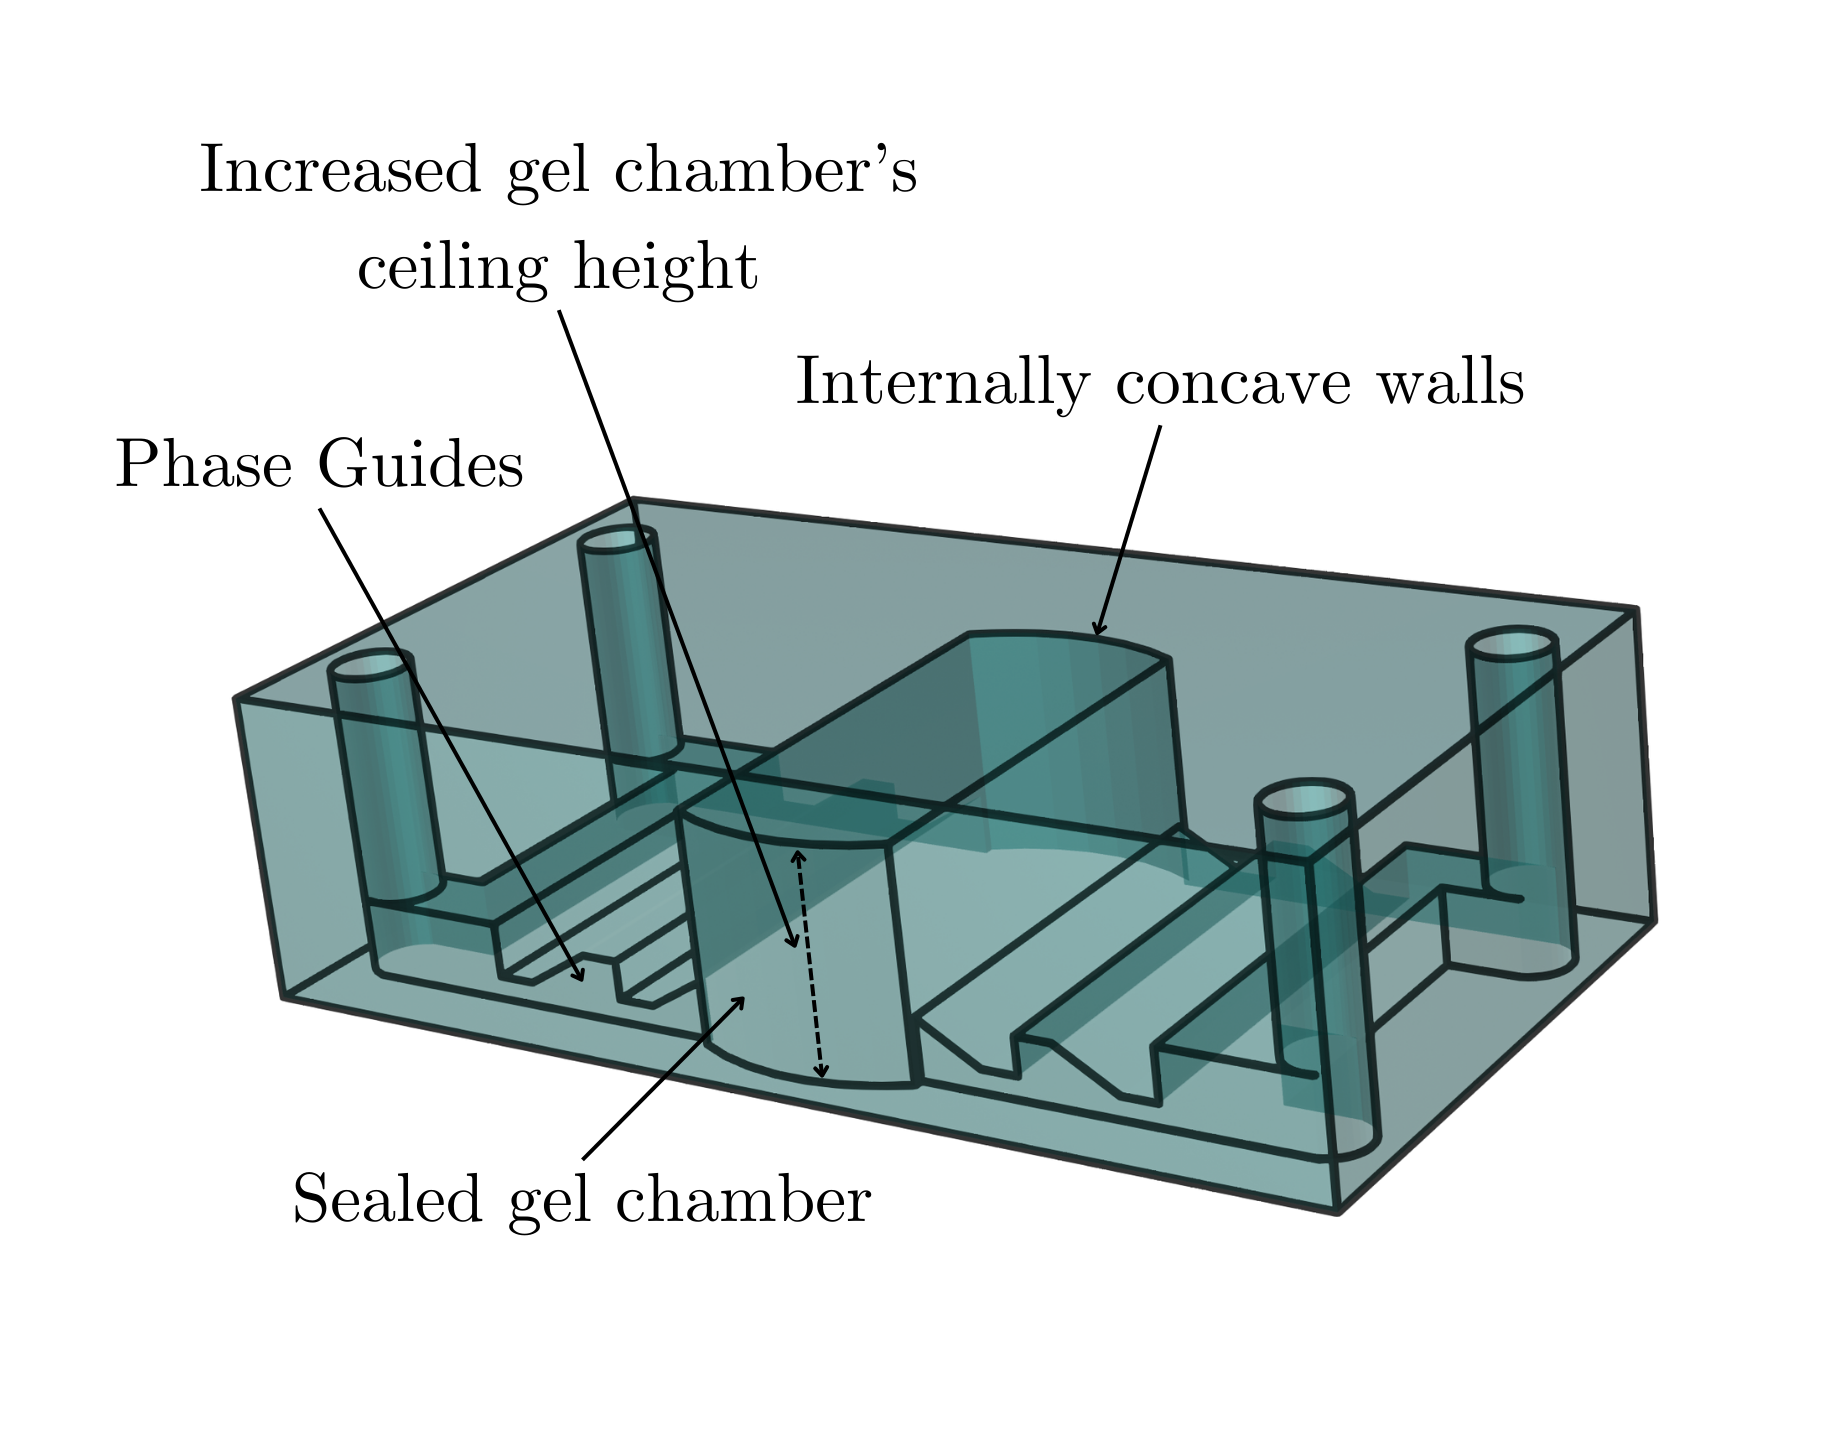
\includegraphics[width=1\linewidth]{dapp_report/figures/final_iter.png}
    \label{fig:final_iter}
    \caption{Annotated graphic of the fifth design iteration displaying important features.}
\end{figure}

\textbf{Features}: Microposts were replaced by phase guides, which were successfully printed. Internally concave walls replaced biconcave structures to accommodate the new phase guides. The ceiling height of the central chamber and the diameter of the side channel inlets were increased to reduce tearing when removing the PDMS mould.

\begin{figure}[!h]
    \centering
    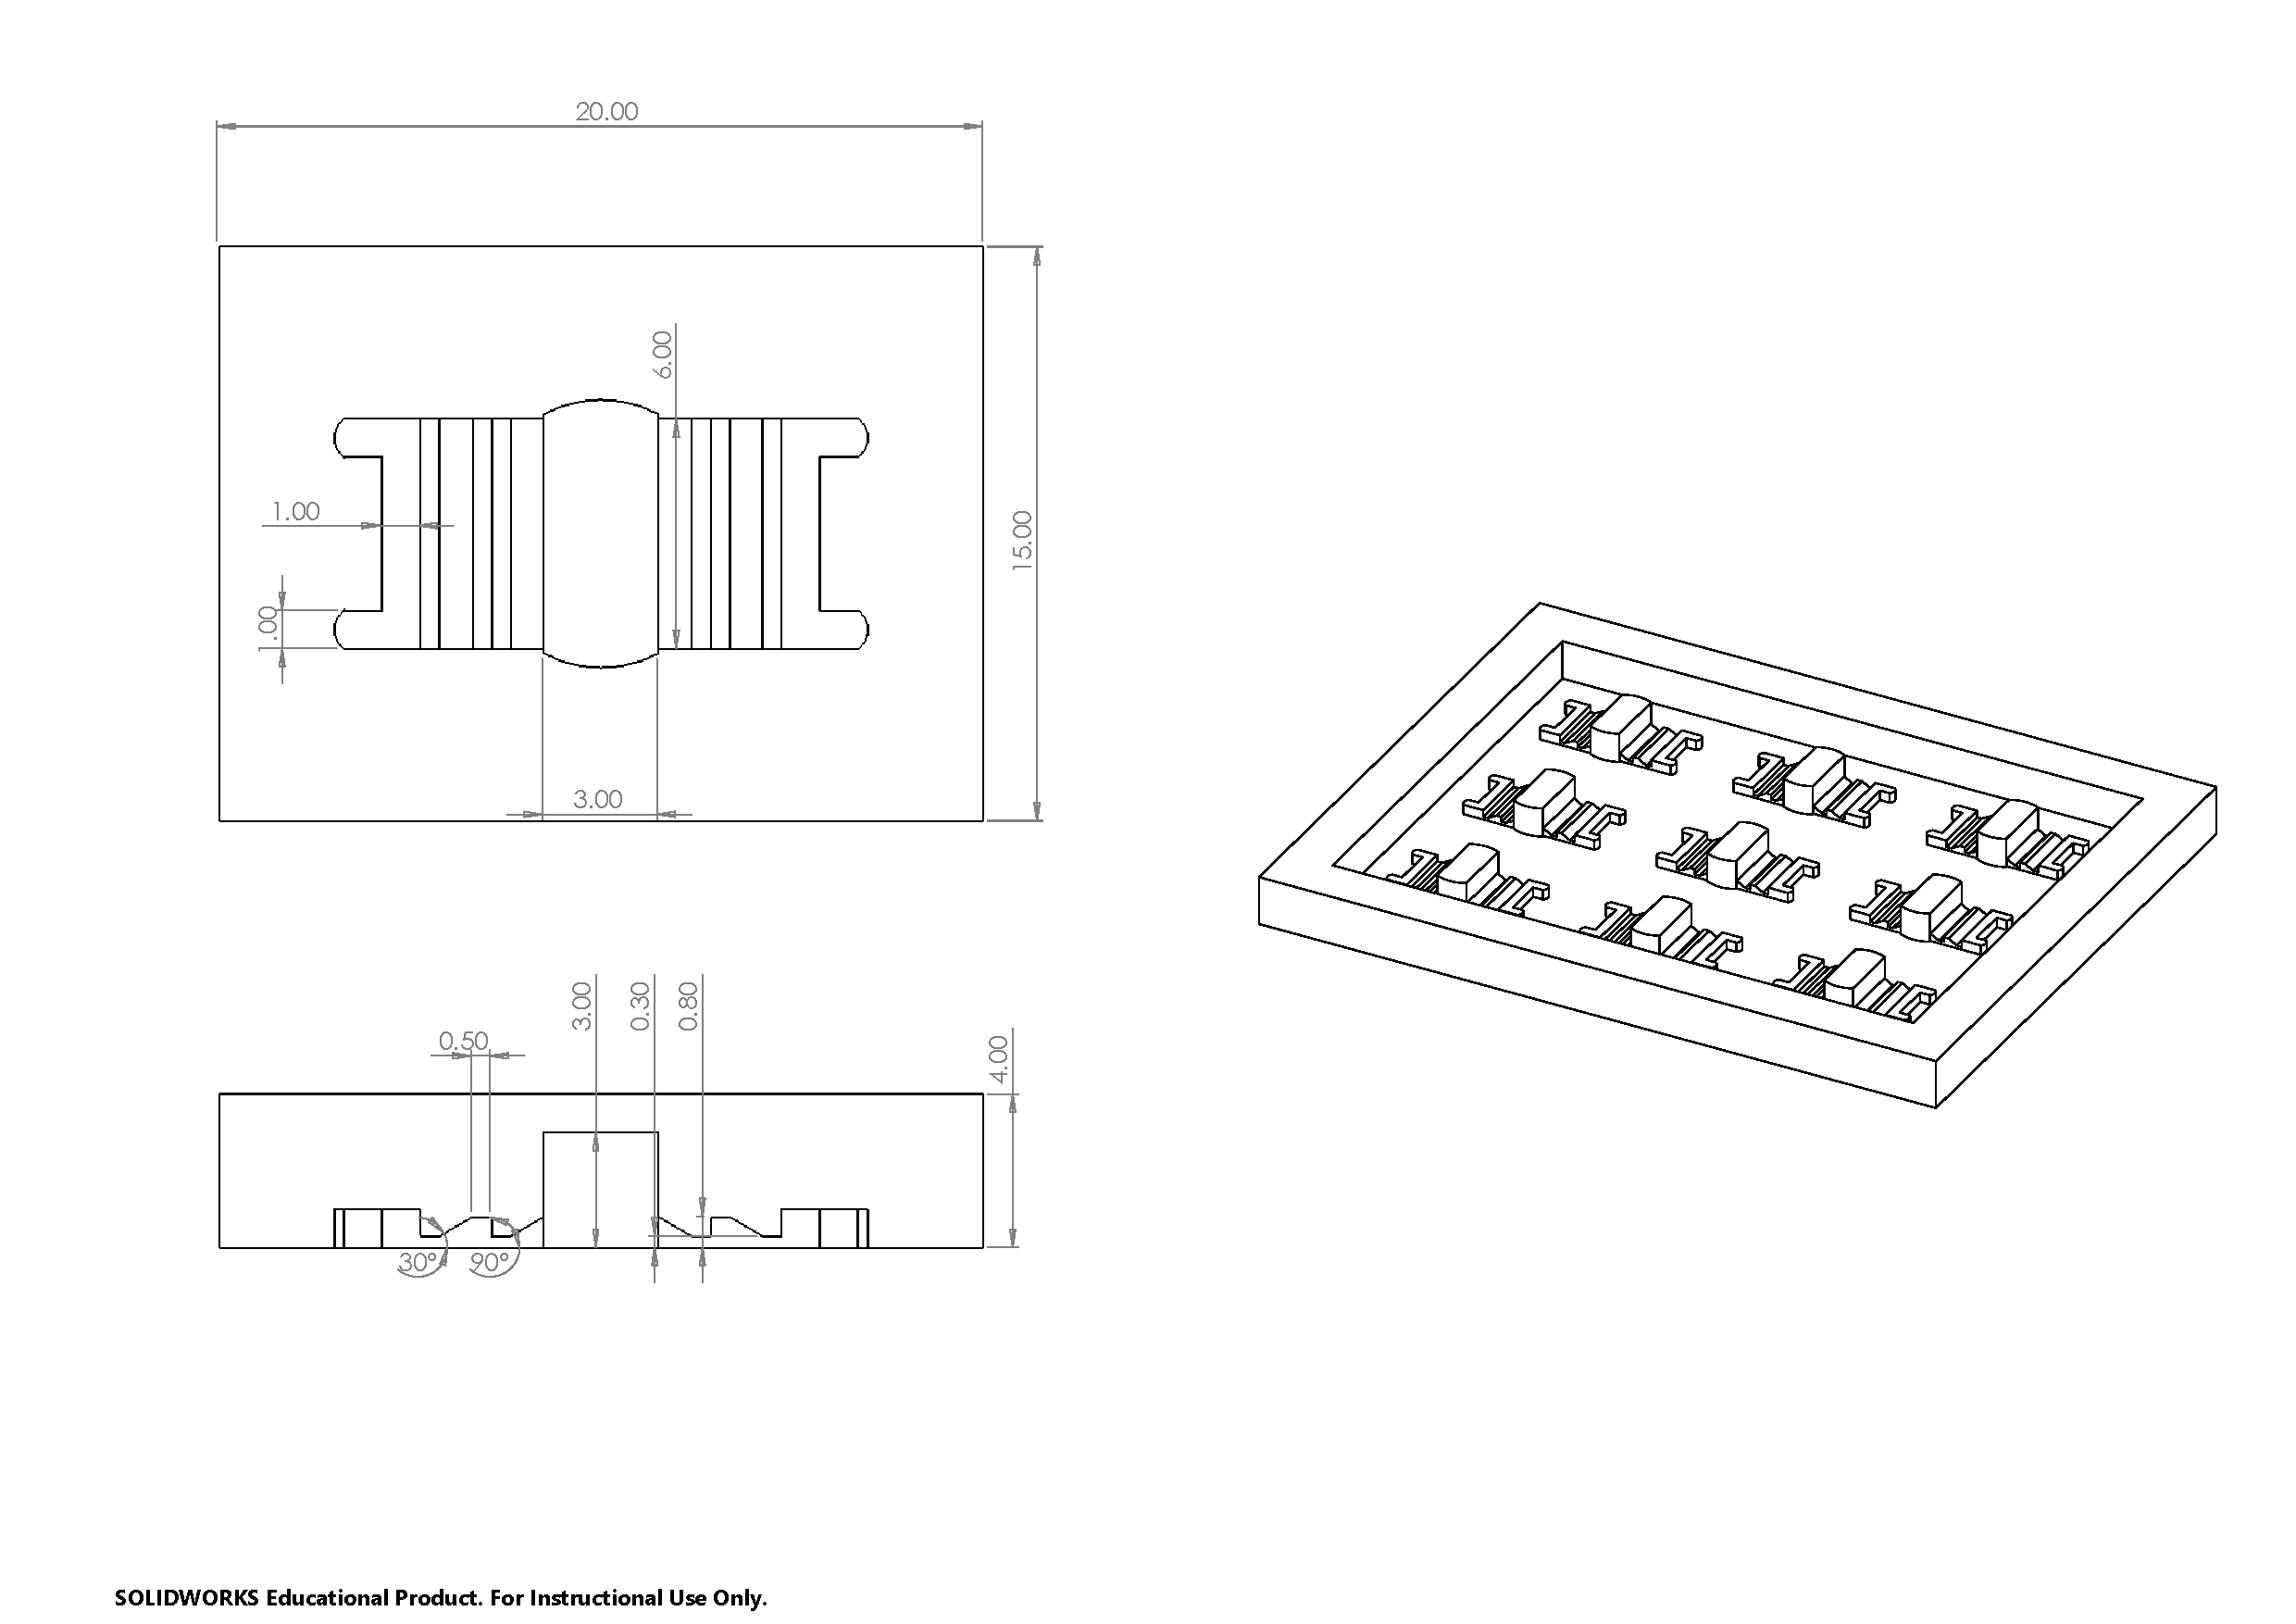
\includegraphics[width=1\linewidth]{PDF/TDV5.pdf}
    \caption{Technical Drawing of the fifth design iteration.}
    \label{fig:TDV5}
\end{figure}

\clearpage





\section{Nomenclature}

~
\begin{table}[!h]
\centering

\begin{tabular}{|m{3cm} |m{14cm} |}
\hline
\textbf{Term} & \textbf{Description}\\
\hline
Angiogenesis  & The growth of new blood vessels from existing vessels  \\
\hline
Biopsy Punch  & A device that can form a tunnel of a specific diameter in a material, usually used to get tissue samples  \\
\hline
Concus-Finn criterion  & It states that for a liquid to favourably fill a microchannel, the contact angle between the liquid and channel walls must be less than 45°  \\
\hline
Cytotoxic  & Toxic to cells  \\
\hline
Dextran dye  & A glucose-derived dye  \\
\hline
Feeder vessel  & Larger diameter capillary that provides a point from which smaller vascular networks can grow  \\
\hline
FFF  & Fused Filament Fabrication: A method of 3D printing, where a thermoplastic filament is extruded out of a heated nozzle to form a layer\\
\hline
Fibrin  & The activated, water-insoluble form of fibrinogen that helps to form blood clots in the body  \\
\hline
Fibrinogen  & A water-soluble protein in blood that is activated for blood clotting  \\
\hline
HUVEC  & Human Umbilical Vein Endothelial Cell  \\
\hline
Hydrogel  & A gel material containing mostly water  \\
\hline

Hydrophobic  & A material property where contact with water results in a contact angle greater than 90°  \\


\hline
Immunofluo- rescence  & A technique that permits visualisation of virtually many components in any given tissue or cell type  \\
\hline
Isopropyl alcohol  & A solvent frequently used in general cleaning  \\
\hline
MSLA  & Masked stereolithography apparatus: a form of resin 3D printing where an LCD screen masks a UV light source to cure a photopolymer resin, varying the exposed shape depending on the layer to be printed  \\
\hline
PAT  & Portable appliance testing  \\
\hline
PBS  & Phosphate buffered saline  \\
\hline
PDMS  & Polydimethylsiloxane, a biocompatible elastomer  \\
\hline
Photopolymer resin  & Highly viscous substance that solidifies upon exposure to UV light of a given wavelength  \\
\hline
PLA  & Polylactic Acid  \\
\hline
Plasma bonding  & Irradiating a surface to plasma in a high oxygen environment to make the surface more reactive to bond to other surfaces  \\
\hline
Thrombin  & The enzyme responsible for converting fibrinogen to fibrin  \\
\hline
Vasculogenesis  & The formation of blood vessels de novo from the differentiation of endothelial cell precursors  \\
\hline
VEGF  & Vascular endothelial growth factor  \\
\hline

\end{tabular}

\end{table}
~
 



\end{document}




